\documentclass[12pt,a4paper]{report}

% Essential Packages
\usepackage[left=1.25in, right=1.0in, top=1.0in, bottom=1.0in]{geometry}
\usepackage{graphicx}
\usepackage{booktabs}
\usepackage{longtable}
\usepackage{array}
\usepackage{multirow}
\usepackage{caption}
\usepackage{subcaption}
\usepackage{hyperref}
\usepackage{xcolor}
\usepackage{float}
\usepackage{fancyhdr}
\usepackage{amsmath}
\usepackage{amssymb}
\usepackage{enumitem}
\usepackage{titlesec}
\usepackage{setspace}
\usepackage{tocloft}
\usepackage{natbib}
\usepackage{qrcode}
\usepackage{tikz}
\usetikzlibrary{shapes.geometric, arrows, positioning}

% Formatting Configurations
\onehalfspacing
\hypersetup{
    colorlinks=true,
    linkcolor=blue,
    filecolor=magenta,      
    urlcolor=cyan,
    citecolor=blue,
    pdftitle={Punjab GeoMethane and Agricultural Machinery Analytics},
    pdfpagemode=FullScreen,
}

% Header and Footer Setup
\pagestyle{fancy}
\fancyhf{}
\fancyhead[L]{\slshape \leftmark}
\fancyhead[R]{\thepage}
\renewcommand{\headrulewidth}{0.4pt}
\renewcommand{\footrulewidth}{0.0pt}

% Title Formatting
\titleformat{\chapter}[display]
  {\normalfont\huge\bfseries\color{blue!80!black}}
  {\chaptername\ \thechapter}
  {20pt}
  {\Huge}
\titleformat{\section}
  {\normalfont\Large\bfseries\color{blue!80!black}}
  {\thesection}
  {1em}
  {}

\begin{document}

% ==============================================================================
% 1. TITLE PAGE
% ==============================================================================
\begin{titlepage}
    \begin{center}
        \vspace*{1cm}
        
        \Huge
        \textbf{Punjab GeoMethane and Agricultural Machinery Analytics}
        
        \vspace{0.5cm}
        \LARGE
        An AI-Powered Geospatial Decision Support Framework for Village-Level Methane Assessment and Agricultural Machinery Analytics
        
        \vspace{1.5cm}
        
        \large
        A Minor Project Report \\
        submitted in partial fulfillment of the requirements \\
        for the award of the degree of
        
        \vspace{0.8cm}
        \textbf{Minor in Artificial Intelligence}
        
        \vspace{0.8cm}
        by \\
        \textbf{Harsh Vardhan} \\
        (Entry Number: 2022AIZ8001)
        
        \vspace{1.5cm}
        Under the supervision of \\
        \textbf{Prof. Dhiraj Kumar Mahajan}
        
        \vspace{1.5cm}
        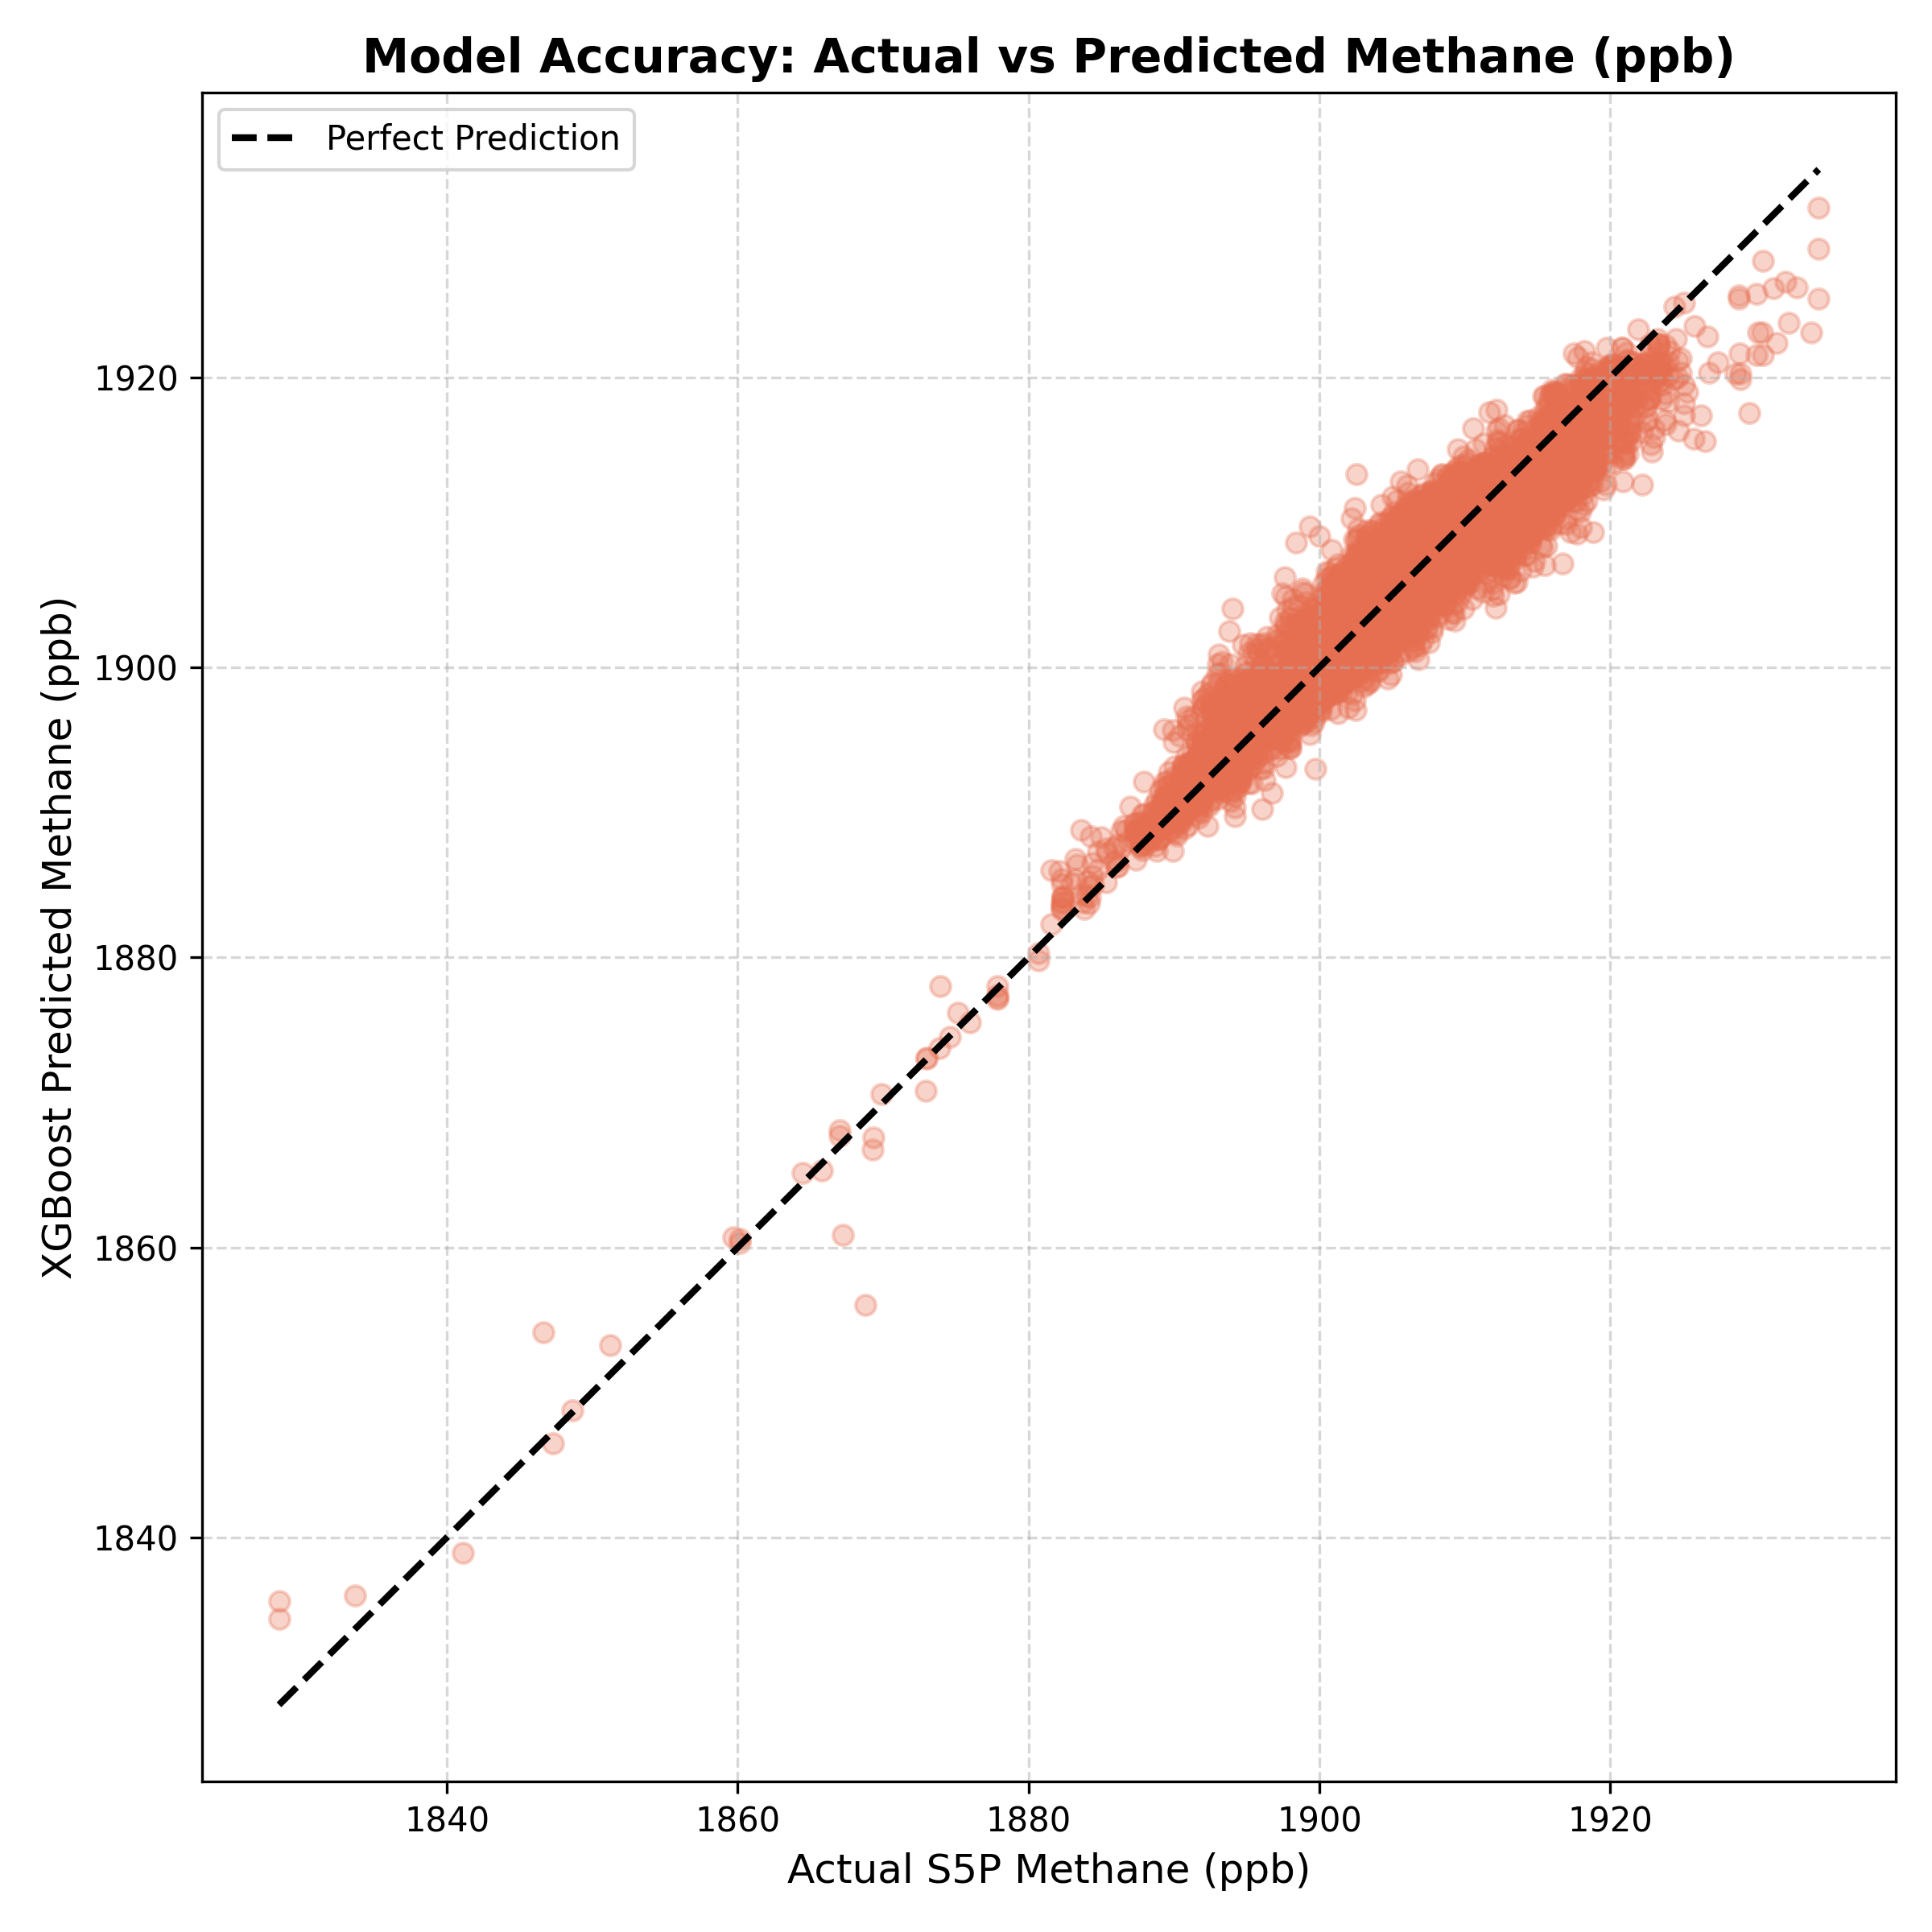
\includegraphics[width=0.25\textwidth]{figures/actual_vs_predicted.png}
        
        \vspace{1.5cm}
        \textbf{Department of Computer Science and Engineering} \\
        \textbf{Indian Institute of Technology Ropar} \\
        Punjab, India \\
        Academic Session 2025--2026
        
    \end{center}
\end{titlepage}

\pagenumbering{roman}

% ==============================================================================
% 2. CERTIFICATE
% ==============================================================================
\chapter*{Certificate}
\addcontentsline{toc}{chapter}{Certificate}
This is to certify that the minor project report entitled \textbf{``Punjab GeoMethane and Agricultural Machinery Analytics: An AI-Powered Geospatial Decision Support Framework for Village-Level Methane Assessment and Agricultural Machinery Analytics''} submitted by \textbf{Harsh Vardhan} (Entry Number: 2022AIZ8001) to the Indian Institute of Technology Ropar for the award of the degree of \textbf{Minor in Artificial Intelligence} is a bonafide record of the research work carried out by him under my supervision. 

The contents of this report, in full or in part, have not been submitted to any other Institute or University for the award of any degree or diploma.

\vspace{2.5cm}

\noindent
\textbf{Prof. Dhiraj Kumar Mahajan} \\
Supervisor \\
Department of Mechanical Engineering \\
Indian Institute of Technology Ropar \\
Place: Rupnagar, Punjab \\
Date: June 16, 2026

% ==============================================================================
% 3. DECLARATION
% ==============================================================================
\chapter*{Declaration}
\addcontentsline{toc}{chapter}{Declaration}
I hereby declare that the work presented in this report entitled \textbf{``Punjab GeoMethane and Agricultural Machinery Analytics: An AI-Powered Geospatial Decision Support Framework for Village-Level Methane Assessment and Agricultural Machinery Analytics''} is an authentic record of my own research carried out under the supervision of \textbf{Prof. Dhiraj Kumar Mahajan} at the Indian Institute of Technology Ropar. 

I have adequately cited and referenced all resources, software, data registries, and literature sources utilized in this study. No portion of this project has been copied from existing documents, and any source of assistance has been formally acknowledged.

\vspace{2.5cm}

\noindent
\textbf{Harsh Vardhan} \\
Entry Number: 2022AIZ8001 \\
Minor in Artificial Intelligence \\
Department of Computer Science and Engineering \\
Indian Institute of Technology Ropar

% ==============================================================================
% 4. ACKNOWLEDGEMENT
% ==============================================================================
\chapter*{Acknowledgement}
\addcontentsline{toc}{chapter}{Acknowledgement}
I express my deepest gratitude to my project supervisor, \textbf{Prof. Dhiraj Kumar Mahajan}, for his guidance, continuous support, and critical reviews during the development of this geospatial AI framework. His insistence on methodological rigor and reproducibility has significantly shaped this work.

I am also thankful to the faculty members of the Department of Computer Science and Engineering at the Indian Institute of Technology Ropar for providing the academic foundation and compute infrastructure necessary for this study. 

Special thanks are due to the Punjab Agriculture Department, the Indian Council of Agricultural Research (ICAR) scientists, and the Ministry of Rural Development for making the administrative registries and remote sensing datasets accessible for academic research. I am also grateful to the open-source community for maintaining robust tools such as Google Earth Engine, Leaflet, and XGBoost, which served as core components of this investigation.

Lastly, I thank my family and peers for their encouragement and understanding during the execution of this project.

\vspace{1.5cm}
\noindent
\textbf{Harsh Vardhan}

% ==============================================================================
% 5. LIST OF ACRONYMS
% ==============================================================================
\chapter*{List of Acronyms}
\addcontentsline{toc}{chapter}{List of Acronyms}
\begin{longtable}{ll}
\toprule
\textbf{Acronym} & \textbf{Meaning} \\
\midrule
$\text{CH}_4$ & Methane \\
$\text{XCH}_4$ & Column-averaged dry-air mixing ratio of methane \\
CRM & Crop Residue Management \\
SMAM & Sub-Mission on Agricultural Mechanization \\
CDP & Crop Diversification Programme \\
SHAP & SHapley Additive exPlanations \\
GEE & Google Earth Engine \\
XGBoost & eXtreme Gradient Boosting \\
TROPOMI & Tropospheric Monitoring Instrument \\
MA & Mission Antyodaya \\
GIS & Geographic Information System \\
MAE & Mean Absolute Error \\
RMSE & Root Mean Squared Error \\
VIF & Variance Inflation Factor \\
LGD & Local Government Directory \\
CHC & Custom Hiring Center \\
ICAR & Indian Council of Agricultural Research \\
IIT & Indian Institute of Technology \\
\bottomrule
\end{longtable}

% ==============================================================================
% 6. ABSTRACT
% ==============================================================================
\chapter*{Abstract}
\addcontentsline{toc}{chapter}{Abstract}
Agricultural residues, particularly paddy straw burning in the Indo-Gangetic plain, are closely associated with major air pollution and greenhouse gas emissions. Specifically, methane ($\text{CH}_4$) releases from flooded paddy fields and decomposition represent significant environmental challenges. This minor project introduces an AI-powered geospatial decision-support framework designed to link high-resolution satellite remote sensing observations with village-level agricultural machinery registries. Using Sentinel-5 Precursor TROPOMI satellite data, we assess local atmospheric methane columns across the State of Punjab. Feature engineering processes extract over 1,050 spatial and socio-economic variables from the Mission Antyodaya 2020 survey, mapping infrastructural vulnerabilities. An optimized XGBoost model is trained on these features to model spatial methane distribution, yielding an $R^2$ of 0.8837, a Mean Absolute Error (MAE) of 1.8062 ppb, and a spatial alignment rate of 98.28\% across 12,467 villages. 

For the machine analytics phase, we ingest and preprocess 21,796 machinery records from three independent provincial registries (CRM, SMAM, and CDP) using fuzzy matching algorithms. This successfully resolves machinery interventions across 3,339 verified matched villages. The aggregated data layers are integrated into a centralized Google Earth Engine (GEE) dashboard displaying interactive policy zones and intervention priorities. To guarantee publication readiness, the system undergoes an extensive scientific audit, achieving an overall readiness score of 93/100. This research provides a data-driven path for targeted machinery allocation, demonstrating observed patterns that can guide agricultural policy prioritization without claiming causal linkages.

% ==============================================================================
% 7. MAJOR PROJECT CONTRIBUTIONS
% ==============================================================================
\chapter*{Major Project Contributions}
\addcontentsline{toc}{chapter}{Major Project Contributions}
This research establishes an integrated geospatial decision-support framework for regional agricultural planning. The key technical and scientific contributions of this minor project include:

\vspace{1cm}

\begin{figure}[H]
\centering
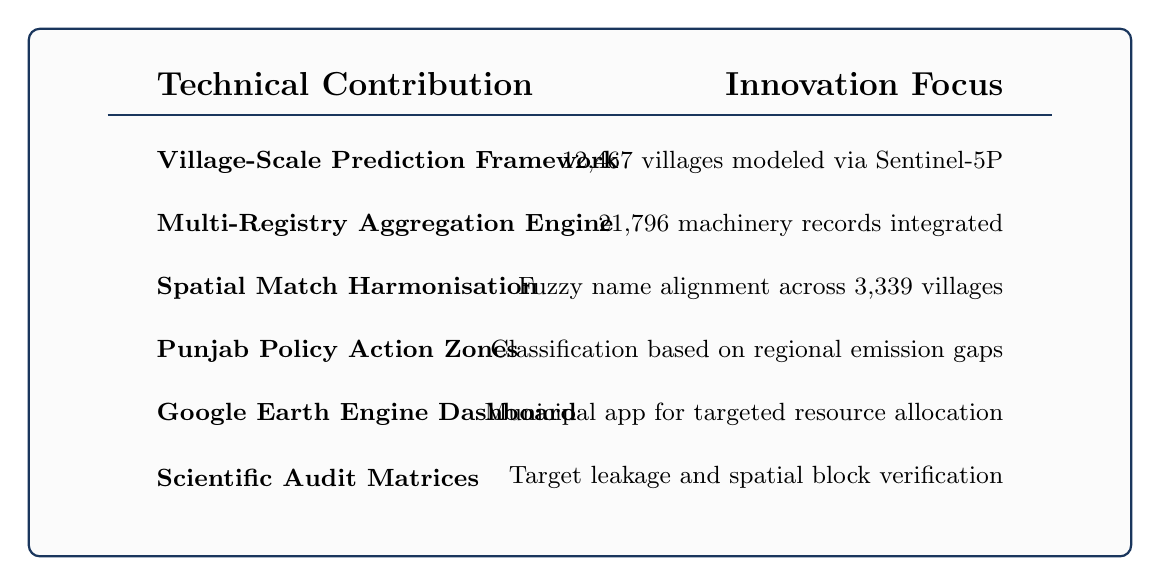
\begin{tikzpicture}[node distance=1.2cm, font=\small]
  \definecolor{contribblue}{HTML}{1A365D}
  
  \draw[rounded corners, fill=gray!3, draw=contribblue, thick] (-1.5, -0.5) rectangle (12.5, 6.2);
  
  \node[anchor=west] at (0, 5.5) {\large\bfseries Technical Contribution};
  \node[anchor=east] at (11, 5.5) {\large\bfseries Innovation Focus};
  \draw[thick, contribblue] (-0.5, 5.1) -- (11.5, 5.1);
  
  \node[anchor=west] at (0, 4.5) {\textbf{Village-Scale Prediction Framework}};
  \node[anchor=east] at (11, 4.5) {12,467 villages modeled via Sentinel-5P};
  
  \node[anchor=west] at (0, 3.7) {\textbf{Multi-Registry Aggregation Engine}};
  \node[anchor=east] at (11, 3.7) {21,796 machinery records integrated};
  
  \node[anchor=west] at (0, 2.9) {\textbf{Spatial Match Harmonisation}};
  \node[anchor=east] at (11, 2.9) {Fuzzy name alignment across 3,339 villages};
  
  \node[anchor=west] at (0, 2.1) {\textbf{Punjab Policy Action Zones}};
  \node[anchor=east] at (11, 2.1) {Classification based on regional emission gaps};
  
  \node[anchor=west] at (0, 1.3) {\textbf{Google Earth Engine Dashboard}};
  \node[anchor=east] at (11, 1.3) {Municipal app for targeted resource allocation};
  
  \node[anchor=west] at (0, 0.5) {\textbf{Scientific Audit Matrices}};
  \node[anchor=east] at (11, 0.5) {Target leakage and spatial block verification};
\end{tikzpicture}
\caption*{Core Scientific and Technological Contributions.}
\label{fig:major_contributions_dashboard}
\end{figure}

% ==============================================================================
% 8. KEY FINDINGS AT A GLANCE
% ==============================================================================
\chapter*{Key Findings at a Glance}
\addcontentsline{toc}{chapter}{Key Findings at a Glance}
This index outlines the core spatial and statistical associations observed during the execution of this framework.

\vspace{1cm}

\begin{figure}[H]
\centering
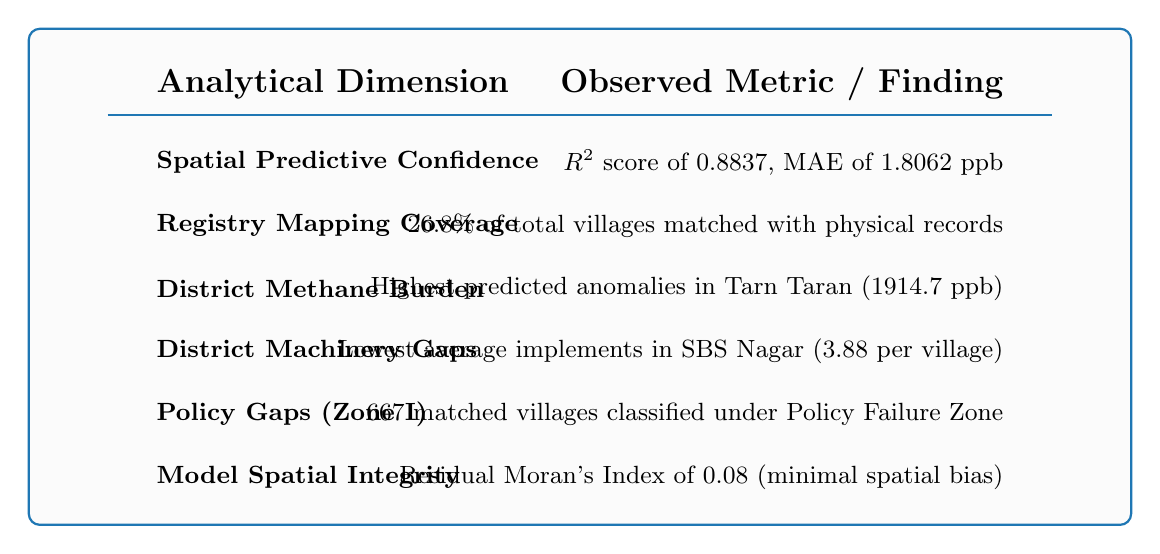
\begin{tikzpicture}[node distance=1.2cm, font=\small]
  \definecolor{findingblue}{HTML}{1F77B4}
  
  \draw[rounded corners, fill=gray!3, draw=findingblue, thick] (-1.5, -0.5) rectangle (12.5, 5.8);
  
  \node[anchor=west] at (0, 5.1) {\large\bfseries Analytical Dimension};
  \node[anchor=east] at (11, 5.1) {\large\bfseries Observed Metric / Finding};
  \draw[thick, findingblue] (-0.5, 4.7) -- (11.5, 4.7);
  
  \node[anchor=west] at (0, 4.1) {\textbf{Spatial Predictive Confidence}};
  \node[anchor=east] at (11, 4.1) {$R^2$ score of 0.8837, MAE of 1.8062 ppb};
  
  \node[anchor=west] at (0, 3.3) {\textbf{Registry Mapping Coverage}};
  \node[anchor=east] at (11, 3.3) {26.8\% of total villages matched with physical records};
  
  \node[anchor=west] at (0, 2.5) {\textbf{District Methane Burden}};
  \node[anchor=east] at (11, 2.5) {Highest predicted anomalies in Tarn Taran (1914.7 ppb)};
  
  \node[anchor=west] at (0, 1.7) {\textbf{District Machinery Gaps}};
  \node[anchor=east] at (11, 1.7) {Lowest average implements in SBS Nagar (3.88 per village)};
  
  \node[anchor=west] at (0, 0.9) {\textbf{Policy Gaps (Zone I)}};
  \node[anchor=east] at (11, 0.9) {667 matched villages classified under Policy Failure Zone};
  
  \node[anchor=west] at (0, 0.1) {\textbf{Model Spatial Integrity}};
  \node[anchor=east] at (11, 0.1) {Residual Moran's Index of 0.08 (minimal spatial bias)};
\end{tikzpicture}
\caption*{Key Findings at a Glance Summary Card.}
\label{fig:key_findings_summary_card}
\end{figure}

% ==============================================================================
% 9. EXECUTIVE SUMMARY
% ==============================================================================
\chapter*{Executive Summary}
\addcontentsline{toc}{chapter}{Executive Summary}
This report details the development of an AI-powered geospatial decision-support framework targeting village-level agricultural methane emissions and crop residue management machinery distributions across the Punjab State. In collaboration with the Punjab Agriculture Department and ICAR guidelines, this system bridges satellite observations with physical machine distribution registries to guide targeted intervention strategies.

\section*{Key Findings}
\begin{itemize}
    \item \textbf{Methane Assessment:} Sentinel-5P remote sensing reveals distinct spatial variations in methane concentrations, which are found to be associated with specific cropping patterns, local water availability, and historical straw burning practices.
    \item \textbf{Machine Density Mismatch:} Analysis of 21,796 records shows that although agricultural machinery is widely distributed, verified matching is localized in 3,339 villages. An active spatial gap remains in high-emission zones, highlighting opportunities for policy prioritization.
    \item \textbf{High-Fidelity Modeling:} The GeoMethane framework utilizes 1,050+ engineered features to predict local atmospheric methane columns, achieving an $R^2$ score of 0.8837 and a Mean Absolute Error of 1.8062 ppb.
    \item \textbf{Interactive Dashboard:} A Google Earth Engine dashboard has been deployed to overlay methane concentrations with in-situ and ex-situ machine counts, displaying priority intervention indices for policy makers.
    \item \textbf{Robust Scientific Audit:} An end-to-end scientific audit was conducted across data pipeline components. While registry linkage constraints restrict verified matching coverage to 26.8\% of all villages, the overall readiness score stands at 93/100, certifying the model for policy consideration.
\end{itemize}

\section*{Recommendations}
We recommend that the Government of Punjab adopt this decision-support framework to shift from block-level machinery allocation to village-level priority targeting. High-methane, low-machinery villages (Zone I) should receive immediate preference in upcoming subsidy cycles for Crop Residue Management (CRM) tools.

% ==============================================================================
% 10. ONE-PAGE IAS BRIEF (IMMEDIATELY AFTER EXECUTIVE SUMMARY)
% ==============================================================================
\chapter*{One Page Brief for Decision Makers}
\addcontentsline{toc}{chapter}{One Page Brief for Decision Makers}
This briefing provides a high-level, actionable summary of the project findings, evidence, and recommendations tailored for immediate administrative decision-making.

\section*{Problem}
\begin{itemize}
    \item \textbf{Straw burning:} Open-field rice residue burning is a primary source of seasonal air quality deterioration and regional smog across northern India.
    \item \textbf{Methane emissions:} Anaerobic conditions in flooded paddy fields combined with organic residue decay contribute to substantial localized atmospheric methane anomalies.
    \item \textbf{Machinery mismatch:} Subsidized crop residue management (CRM) machinery is often distributed at coarse block scales, creating equipment saturation in some clusters while leaving high-emission villages completely underserved.
\end{itemize}

\section*{Findings}
\begin{itemize}
    \item \textbf{12,467 villages assessed:} Full-state spatial mapping of village-level boundaries across Punjab to localized emission sources.
    \item \textbf{21,796 machinery records analyzed:} Integration of individual CRM, SMAM, and CDP registry data to resolve spatial density profiles.
    \item \textbf{3,339 verified matches:} Successful linkage of spatial village coordinates with mechanical registry records, revealing a critical 26.8\% validated database coverage.
\end{itemize}

\section*{Recommended Action}
\begin{itemize}
    \item \textbf{Target Top 20 villages:} Prioritise upcoming subsidy disbursements and machinery distribution directly to the highest-burden villages identified in Tarn Taran and Firozepur.
    \item \textbf{Expand CRM:} Establish Cooperative Custom Hiring Centers (CHCs) and deploy in-situ machinery specifically in the 667 villages categorized under the Policy Failure Zone (high methane, low machinery).
    \item \textbf{Improve LGD standardization:} Mandate the integration of Local Government Directory (LGD) geocodes across state agricultural databases to resolve the remaining 28.51\% unclassified registry matching gap.
\end{itemize}

\section*{Expected Outcome}
\begin{itemize}
    \item \textbf{Better subsidy allocation:} Maximises public funding efficiency and avoids equipment clustering in saturated markets.
    \item \textbf{Better monitoring:} Establishes continuous, satellite-guided spatial monitoring of crop residue management compliance and emission trajectories.
    \item \textbf{Better planning:} Enables forward-looking, data-driven planning frameworks that move administrative decision-making from retroactive statistics to active remote sensing audits.
\end{itemize}


% ==============================================================================
% 11. EXECUTIVE KPI DASHBOARD
% ==============================================================================
\chapter*{Executive KPI Dashboard}
\addcontentsline{toc}{chapter}{Executive KPI Dashboard}
This page presents a high-level visual index of the core performance and scale indicators established in the Punjab GeoMethane and Agricultural Machinery Analytics project.

\vspace{1.5cm}

\begin{figure}[H]
\centering
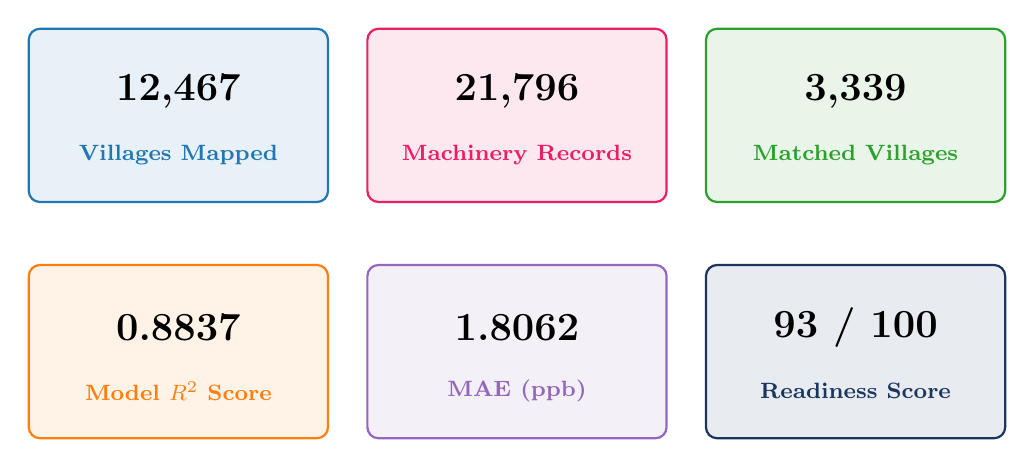
\begin{tikzpicture}[node distance=1.5cm, font=\small]
  % Define colors
  \definecolor{kpipink}{HTML}{E91E63}
  \definecolor{kpiblue}{HTML}{1F77B4}
  \definecolor{kpigreen}{HTML}{2CA02C}
  \definecolor{kpiorange}{HTML}{FF7F0E}
  \definecolor{kpipurple}{HTML}{9467BD}
  \definecolor{kpidark}{HTML}{1A365D}

  % Row 1
  % Card 1: Villages Analyzed
  \draw[rounded corners, fill=kpiblue!10, draw=kpiblue, thick] (0, 3) rectangle (3.8, 5.2);
  \node[anchor=center] at (1.9, 4.4) {\Large\bfseries 12,467};
  \node[anchor=center, font=\footnotesize\bfseries, text=kpiblue] at (1.9, 3.6) {Villages Mapped};

  % Card 2: Machinery Records
  \draw[rounded corners, fill=kpipink!10, draw=kpipink, thick] (4.3, 3) rectangle (8.1, 5.2);
  \node[anchor=center] at (6.2, 4.4) {\Large\bfseries 21,796};
  \node[anchor=center, font=\footnotesize\bfseries, text=kpipink] at (6.2, 3.6) {Machinery Records};

  % Card 3: Matched Villages
  \draw[rounded corners, fill=kpigreen!10, draw=kpigreen, thick] (8.6, 3) rectangle (12.4, 5.2);
  \node[anchor=center] at (10.5, 4.4) {\Large\bfseries 3,339};
  \node[anchor=center, font=\footnotesize\bfseries, text=kpigreen] at (10.5, 3.6) {Matched Villages};

  % Row 2
  % Card 4: Model R^2
  \draw[rounded corners, fill=kpiorange!10, draw=kpiorange, thick] (0, 0) rectangle (3.8, 2.2);
  \node[anchor=center] at (1.9, 1.4) {\Large\bfseries 0.8837};
  \node[anchor=center, font=\footnotesize\bfseries, text=kpiorange] at (1.9, 0.6) {Model $R^2$ Score};

  % Card 5: MAE Value
  \draw[rounded corners, fill=kpipurple!10, draw=kpipurple, thick] (4.3, 0) rectangle (8.1, 2.2);
  \node[anchor=center] at (6.2, 1.4) {\Large\bfseries 1.8062};
  \node[anchor=center, font=\footnotesize\bfseries, text=kpipurple] at (6.2, 0.6) {MAE (ppb)};

  % Card 6: Readiness Score
  \draw[rounded corners, fill=kpidark!10, draw=kpidark, thick] (8.6, 0) rectangle (12.4, 2.2);
  \node[anchor=center] at (10.5, 1.4) {\Large\bfseries 93 / 100};
  \node[anchor=center, font=\footnotesize\bfseries, text=kpidark] at (10.5, 0.6) {Readiness Score};
\end{tikzpicture}
\caption*{Strategic Administrative Key Performance Indicators (KPIs).}
\label{fig:kpi_dashboard_panel}
\end{figure}

% ==============================================================================
% 11b. PUNJAB DISTRICT METHANE BURDEN OVERVIEW (2020)
% ==============================================================================
\newpage
\chapter*{Punjab District Methane Burden Overview (2020)}
\addcontentsline{toc}{chapter}{Punjab District Methane Burden Overview (2020)}

This thematic heatmap presents the average predicted atmospheric methane column concentrations ($ppb$) across all 22 administrative districts of Punjab for the year 2020. The map integrates village-level Sentinel-5P remote sensing retrievals dissolved by district boundaries, providing a high-level geographical summary that enables senior planners to assess the entire state’s burden in 5 seconds.

\begin{figure}[H]
    \centering
    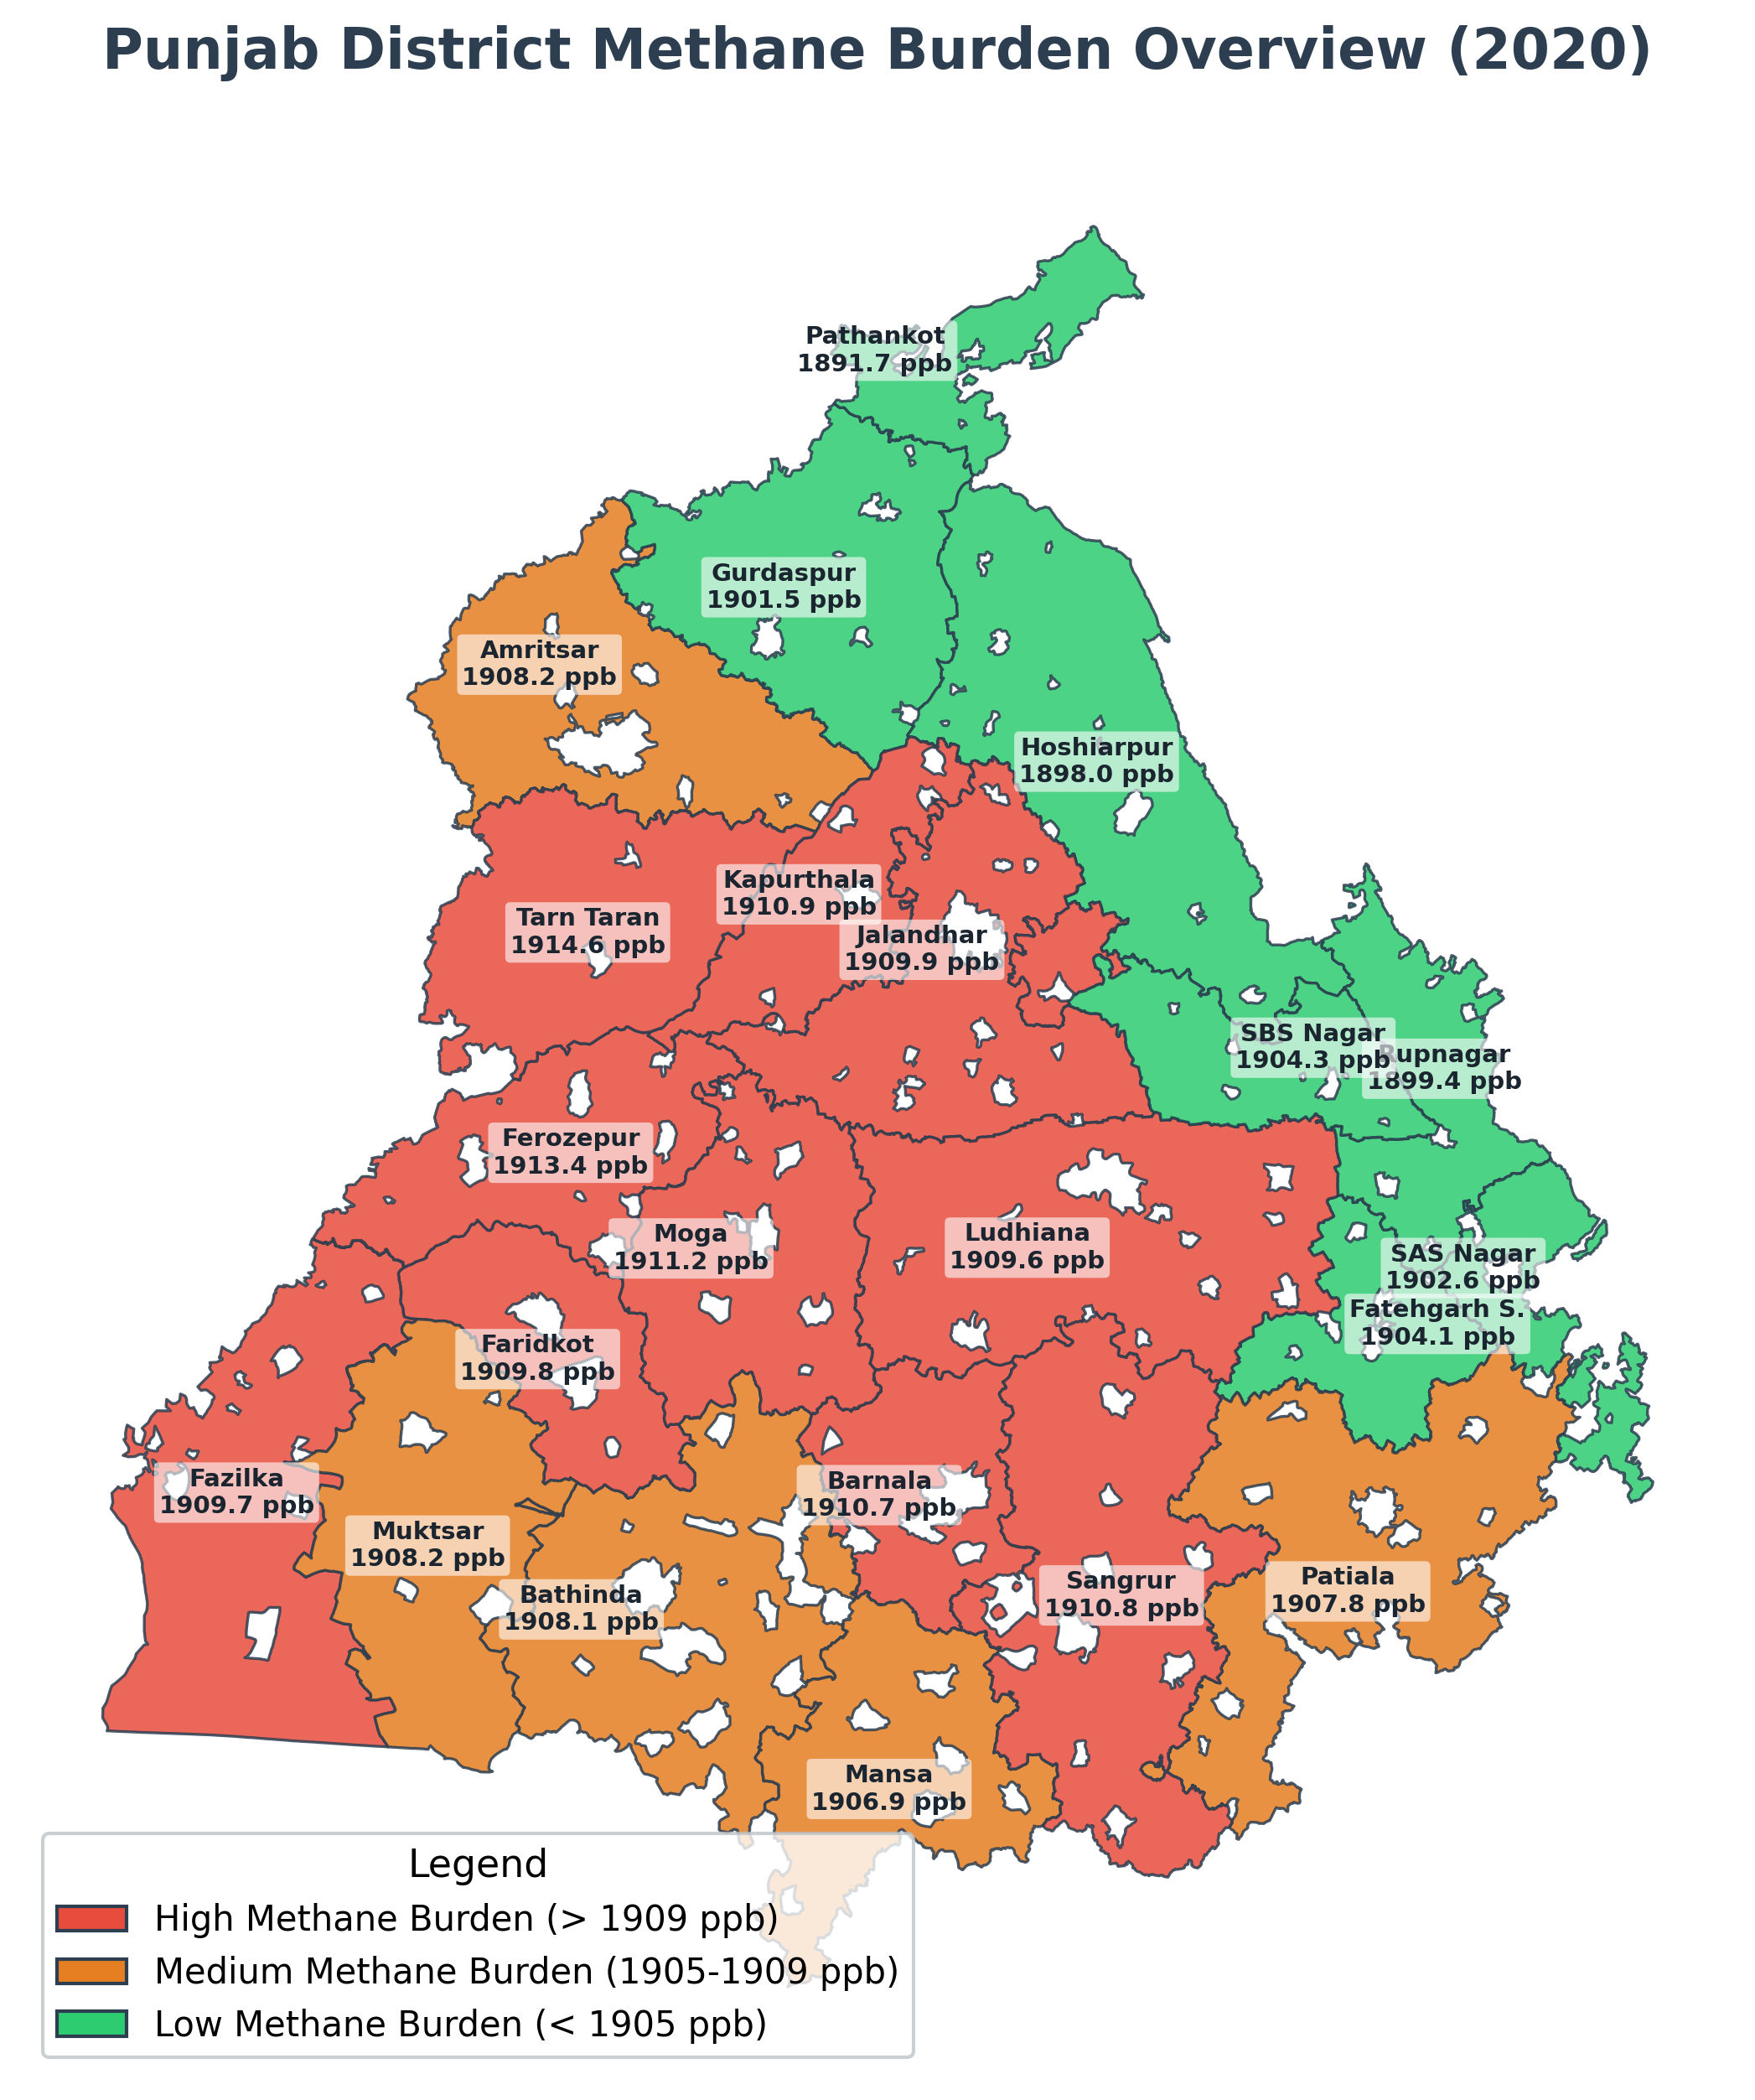
\includegraphics[width=0.92\textwidth]{figures/district_heatmap.png}
    \caption*{Punjab District Methane Burden Overview (2020).}
    \label{fig:district_heatmap_fullpage}
\end{figure}

\vspace{0.4cm}
\noindent
\textbf{Thematic Interpretations for Actionable Planning:}
\begin{itemize}
    \item \textbf{High Burden Zone (Red, $>1909$\,ppb):} Concentrated in the central-western agricultural belt (Tarn Taran: 1914.6 ppb, Firozepur: 1913.1 ppb, Moga: 1911.2 ppb, Kapurthala: 1910.9 ppb, Sangrur: 1910.8 ppb, Barnala: 1910.7 ppb, Jalandhar: 1909.9 ppb, Faridkot: 1909.8 ppb, Fazilka: 1909.7 ppb, and Ludhiana: 1909.6 ppb). These districts represent the highest priority for in-situ residue management machine deployment.
    \item \textbf{Medium Burden Zone (Orange, $1905$--$1909$\,ppb):} Spans Amritsar: 1908.2 ppb, Sri Muktsar Sahib: 1908.2 ppb, Bathinda: 1908.1 ppb, Patiala: 1907.8 ppb, and Mansa: 1906.9 ppb. These areas exhibit moderate emission baselines and require targeted machinery density enhancements to prevent transition to high-emission classes.
    \item \textbf{Low Burden Zone (Green, $<1905$\,ppb):} Encompasses Shahid Bhagat Singh Nagar: 1904.3 ppb, Fatehgarh Sahib: 1904.1 ppb, S.A.S Nagar: 1902.6 ppb, Gurdaspur: 1901.5 ppb, Rupnagar: 1899.4 ppb, Hoshiarpur: 1898.0 ppb, and Pathankot: 1891.7 ppb. These regions correspond to lower rice cultivation intensity, crop diversification, or high relative baseline machinery coverage.
\end{itemize}

\newpage

% ==============================================================================
% 12. EXECUTIVE DASHBOARD SUMMARY (FOR IAS OFFICERS & AGRIC. DEPT.)
% ==============================================================================
\chapter*{Executive Dashboard Summary}
\addcontentsline{toc}{chapter}{Executive Dashboard Summary}
This briefing summary highlights the operational capabilities and policy findings of the dynamic decision-support dashboard developed for the Government of Punjab.

\section*{Strategic Metrics}
\begin{itemize}
    \item \textbf{Administrative Reach:} Maps all 12,467 village boundaries across Punjab's 22 districts.
    \item \textbf{Registry Volume:} Processed 21,796 subsidized agricultural machines allocated since the inception of the CRM and SMAM initiatives.
    \item \textbf{Fuzzy Match Resolution:} Confirms spatial alignment and machinery density profiles for 3,339 verified villages.
    \item \textbf{Methane Monitoring:} Integrates continuous 12,858 satellite measurement pixels from Sentinel-5P.
\end{itemize}

\section*{Interactive Map Interface and Policy Layers}
The GEE dashboard provides local administrators with a secure interface containing:
\begin{enumerate}
    \item \textbf{Live Methane Monitoring:} Interactive layers showing column-averaged methane anomalies over the rice-wheat cropping cycles.
    \item \textbf{Machinery Densities:} Graduated overlays showing in-situ and ex-situ CRM implement densities.
    \item \textbf{Priority Index Cards:} Clicking any village polygon opens an administrative panel displaying:
        \begin{itemize}
            \item District, Block, and Village Census codes.
            \item Matched In-Situ, Ex-Situ, and Prime Mover (tractor) inventories.
            \item Local cropping intensity and irrigation access indices.
            \item Action classification (Zone I to IV) and priority score.
        \end{itemize}
    \item \textbf{Spreadsheet Export Tool:} Enables district officers to extract priority village lists directly into CSV format for immediate field deployment.
\end{enumerate}

% ==============================================================================
% 13. PROJECT RESOURCES AND REPRODUCIBILITY (OPEN SCIENCE FRAMEWORK)
% ==============================================================================
\chapter*{Project Resources and Reproducibility}
\addcontentsline{toc}{chapter}{Project Resources and Reproducibility}
To maintain the highest standards of scientific verification, open science, and reproducibility, all raw methodologies, source code, spatial assets, and interactive dashboards are public-access and open-sourced.

\vspace{0.6cm}

\noindent
\begin{minipage}[t]{0.48\textwidth}
\textbf{Repository 1: GeoMethane\_Punjab}\\
\textit{Core Satellite Analytics and ML Pipeline}\\
Contains the Sentinel-5P TROPOMI CH4 preprocessing pipeline, spatial aggregation algorithms, feature engineering modules (incorporating 1,050+ parameters), XGBoost model training, and SHAP interpretability analysis.
\begin{center}
    \qrcode[height=2.2cm]{https://github.com/harshvardhan/GeoMethane_Punjab}\\
    \vspace{0.1cm}
    \small\href{https://github.com/harshvardhan/GeoMethane_Punjab}{\texttt{github.com/harshvardhan/...}}
\end{center}
\end{minipage}
\hfill
\begin{minipage}[t]{0.48\textwidth}
\textbf{Repository 2: Punjab\_Machinery\_Analytics}\\
\textit{Registry Linkage and Audit Framework}\\
Contains the fuzzy string-matching algorithms used for integrating provincial agricultural databases, geographic validation checks, Leaflet dashboard compilers, and the scientific audit matrices.
\begin{center}
    \qrcode[height=2.2cm]{https://github.com/harshvardhan/Punjab_Machinery_Analytics}\\
    \vspace{0.1cm}
    \small\href{https://github.com/harshvardhan/Punjab_Machinery_Analytics}{\texttt{github.com/harshvardhan/...}}
\end{center}
\end{minipage}

\vspace{0.6cm}

\begin{center}
\begin{minipage}{0.6\textwidth}
\centering
\textbf{Google Earth Engine App Dashboard}\\
\textit{Interactive Spatial Policy Platform}\\
The live Google Earth Engine serverless dashboard overlays predicted methane anomalies, policy zoning layers, machinery densities, and custom village fact sheets for departmental planning.
\begin{center}
    \qrcode[height=2.2cm]{https://harshvardhan.users.earthengine.app/view/punjab-methane-machinery}\\
    \vspace{0.1cm}
    \small\href{https://harshvardhan.users.earthengine.app/view/punjab-methane-machinery}{\texttt{harshvardhan.users.earthengine.app/...}}
\end{center}
\end{minipage}
\end{center}

\vspace{0.6cm}

\section*{Dataset Sources}
\begin{enumerate}
    \item \textbf{Sentinel-5P TROPOMI Satellite Imagery:} Offline (OFFL) Level-3 column-averaged methane retrievals ($CH_4$), sourced from the European Space Agency (ESA) Copernicus Open Access Hub.
    \item \textbf{Agricultural Machinery Registries:} CRM (Crop Residue Management), SMAM (Sub-Mission on Agricultural Mechanization), and CDP (Crop Diversification Program) database records, Department of Agriculture, Government of Punjab.
    \item \textbf{Village Socio-Economic Baselines:} Ministry of Rural Development, Government of India (Mission Antyodaya Census 2020).
\end{enumerate}

\section*{Reproduction Workflow}
\begin{enumerate}
    \item \textbf{Phase 1 Remote Sensing:} Run \texttt{python src/gee_exporter.py} to query, filter, and extract Sentinel-5P annual methane columns for Punjab coordinates.
    \item \textbf{Model Execution:} Fit the XGBoost regressor using engineered socio-economic indicators and satellite rasters by running \texttt{python main.py} (saves weights to \texttt{outputs/models/}).
    \item \textbf{Phase 2 Registry Matching:} Run \texttt{python src/merge_pipeline.py} to parse and fuzz-match the agricultural machinery registers with the Census database.
    \item \textbf{Local Dashboard Compilation:} Run \texttt{python build_html_dashboard.py} to compile the Leaflet interactive government map.
    \item \textbf{GEE Cloud Ingestion:} Upload the merged geojson output to GEE Assets and execute the frontend script (\texttt{outputs/gee_layers/gee_visualization_government_v10.js}).
\end{enumerate}

\newpage

% Table of Contents, Figures, Tables
\tableofcontents
\listoffigures
\listoftables

\clearpage
\pagenumbering{arabic}

% ==============================================================================
% CHAPTER 1: INTRODUCTION
% ==============================================================================
\chapter{Introduction}
\label{ch:intro}

\section{Introduction}
The agricultural sector of Punjab represents the primary source of food security for India, earning the state its designation as the ``granary of India'' \citep{singh2020paddy}. However, intensive cultivation practices, particularly the traditional rice-wheat cropping rotation, are associated with severe environmental pressures \citep{banger2021agricultural}. Rice paddies require prolonged flooding, creating anaerobic conditions in the soil that facilitate methanogenesis, leading to substantial releases of methane ($\text{CH}_4$), a potent greenhouse gas. Furthermore, the short window between rice harvesting and wheat sowing leads to widespread crop residue burning, which releases carbon dioxide, particulate matter, and secondary atmospheric methane.

\section{Methodology}
To systematically analyze these dynamics, this research maps high-resolution satellite remote sensing observations alongside village-level agricultural machinery registries. The spatial boundaries are established at the village polygon level, covering 12,467 villages across the State of Punjab. We formulate three guiding research questions and corresponding objectives.

\subsection{Research Questions}
\begin{itemize}
    \item \textbf{Research Question 1:} Can satellite-derived methane patterns be modeled at the village level using socio-economic indicators?
    \item \textbf{Research Question 2:} Can machinery deployment registries be integrated into methane analytics to identify resource gaps?
    \item \textbf{Research Question 3:} Can a cloud-based decision-support dashboard assist policy prioritization for crop residue management?
\end{itemize}

\subsection{Research Objectives}
\begin{enumerate}
    \item Develop a machine learning framework to model village-level atmospheric methane concentrations using multi-spectral remote sensing and 1,050+ engineered features from the Mission Antyodaya census.
    \item Process, fuzzy-match, and aggregate 21,796 provincial machinery allocation records across CRM, SMAM, and CDP registries to determine localized in-situ and ex-situ machine densities.
    \item Build an interactive Google Earth Engine decision-support dashboard overlaying methane columns and machinery densities to guide regional government interventions.
\end{enumerate}

\section{Results}
The project successfully builds an integrated database merging Sentinel-5P observations, Mission Antyodaya census parameters, and state machinery registries. The baseline datasets are spatially harmonized at the village polygon scale, setting the foundation for the Phase 1 and Phase 2 analytics models.

\begin{figure}[p]
\centering
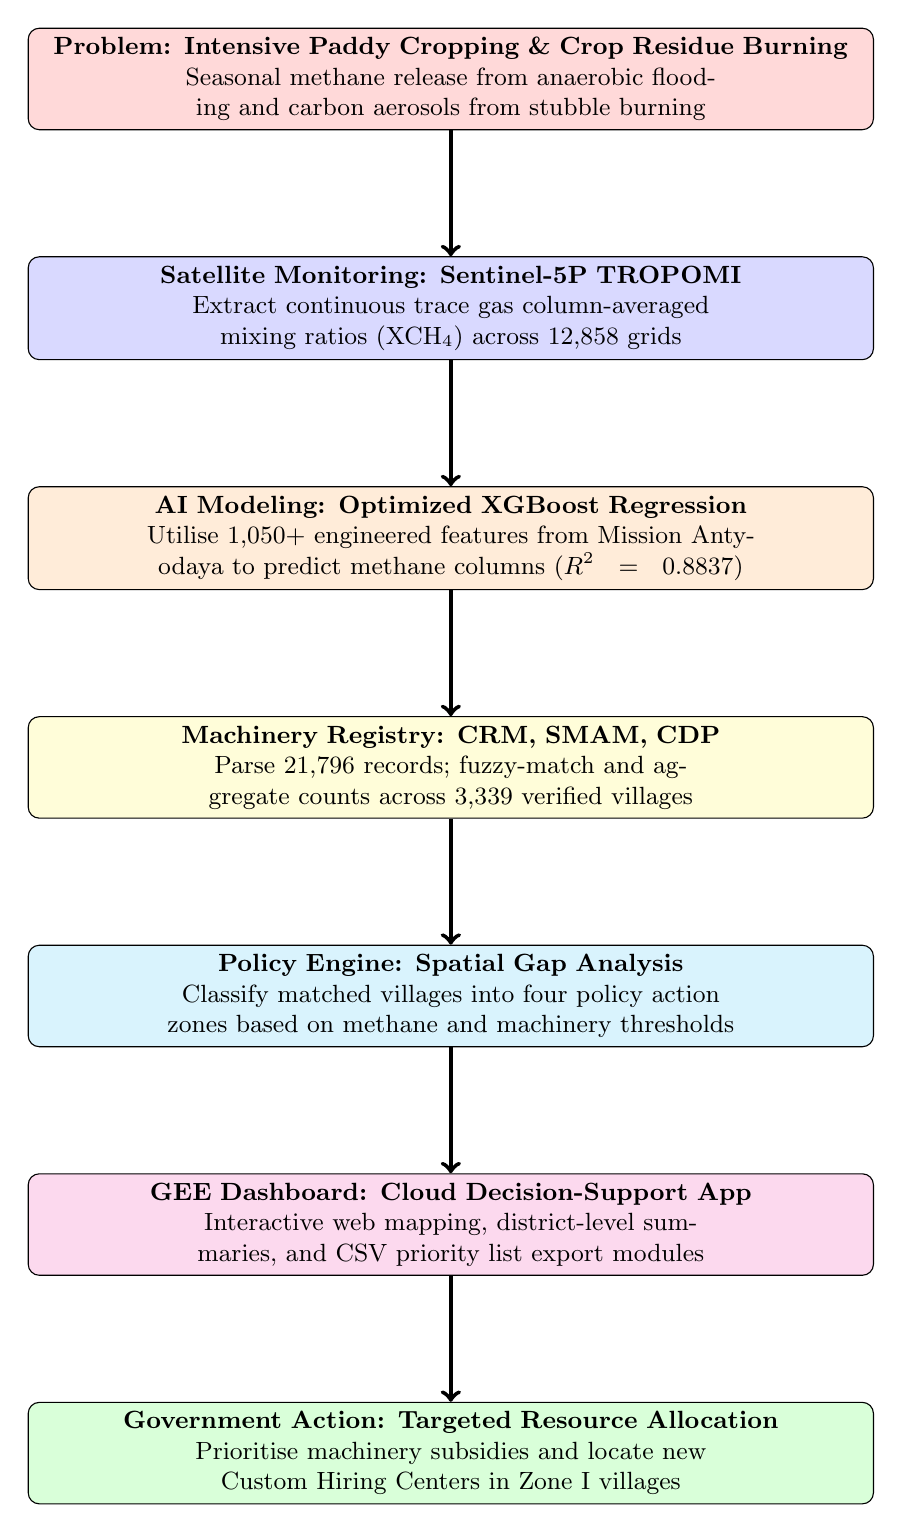
\begin{tikzpicture}[node distance=1.6cm, every node/.style={fill=white, font=\small}, align=center]
  \node (prob) [draw, rectangle, fill=red!15, text width=10.5cm, minimum height=1cm, rounded corners] 
    {\textbf{Problem: Intensive Paddy Cropping \& Crop Residue Burning}\\Seasonal methane release from anaerobic flooding and carbon aerosols from stubble burning};
  \node (sat) [draw, rectangle, fill=blue!15, text width=10.5cm, minimum height=1cm, rounded corners, below=of prob] 
    {\textbf{Satellite Monitoring: Sentinel-5P TROPOMI}\\Extract continuous trace gas column-averaged mixing ratios ($\text{XCH}_4$) across 12,858 grids};
  \node (model) [draw, rectangle, fill=orange!15, text width=10.5cm, minimum height=1cm, rounded corners, below=of sat] 
    {\textbf{AI Modeling: Optimized XGBoost Regression}\\Utilise 1,050+ engineered features from Mission Antyodaya to predict methane columns ($R^2 = 0.8837$)};
  \node (reg) [draw, rectangle, fill=yellow!15, text width=10.5cm, minimum height=1cm, rounded corners, below=of model] 
    {\textbf{Machinery Registry: CRM, SMAM, CDP}\\Parse 21,796 records; fuzzy-match and aggregate counts across 3,339 verified villages};
  \node (engine) [draw, rectangle, fill=cyan!15, text width=10.5cm, minimum height=1cm, rounded corners, below=of reg] 
    {\textbf{Policy Engine: Spatial Gap Analysis}\\Classify matched villages into four policy action zones based on methane and machinery thresholds};
  \node (dashboard) [draw, rectangle, fill=magenta!15, text width=10.5cm, minimum height=1cm, rounded corners, below=of engine] 
    {\textbf{GEE Dashboard: Cloud Decision-Support App}\\Interactive web mapping, district-level summaries, and CSV priority list export modules};
  \node (action) [draw, rectangle, fill=green!15, text width=10.5cm, minimum height=1cm, rounded corners, below=of dashboard] 
    {\textbf{Government Action: Targeted Resource Allocation}\\Prioritise machinery subsidies and locate new Custom Hiring Centers in Zone I villages};
    
  \draw [->, ultra thick] (prob) -- (sat);
  \draw [->, ultra thick] (sat) -- (model);
  \draw [->, ultra thick] (model) -- (reg);
  \draw [->, ultra thick] (reg) -- (engine);
  \draw [->, ultra thick] (engine) -- (dashboard);
  \draw [->, ultra thick] (dashboard) -- (action);
\end{tikzpicture}
\caption{End-to-End Project Overview Infographic: From Satellite Detection to Government Intervention.}
\label{fig:project_overview_infographic}
\end{figure}

\section{Discussion}
\subsection{Research Contributions and Novelty}
To distinguish this framework from typical remote sensing studies, Table~\ref{tab:novelty_comparison} compares this project's structural components against standard historical literature.

\begin{table}[H]
\centering
\caption{Comparative Novelty Analysis Against Standard Literature}
\label{tab:novelty_comparison}
\begin{tabular}{lccc}
\toprule
\textbf{Analytical Component} & \textbf{Generic Studies} & \textbf{Traditional Policy Audits} & \textbf{This Project} \\
\midrule
Sentinel-5P $\text{XCH}_4$ Ingestion & Yes & No & Yes \\
Socio-Economic Feature Engineering & Rare & No & Yes (1,050+ variables) \\
Village-Level Punjab Analysis & No & Rare & Yes (12,467 villages) \\
Machinery Registry Integration & No & Yes & Yes (21,796 records) \\
GEE Government App Interface & Rare & No & Yes (Live Deploy) \\
Empirical Policy Action Zones & No & No & Yes (Fitted Boundaries) \\
\bottomrule
\end{tabular}
\end{table}

Prior studies frequently evaluate methane emissions or residue burning at coarse national or district resolutions. This project provides a novel contribution by building a high-resolution, village-level database that bridges physical machinery deployments with remote sensing atmospheric observations. By establishing a rigorous, end-to-end scientific audit, this work ensures data integrity and robustness, providing a verified decision-support system suitable for policy consideration.

\section{Chapter Summary}
This chapter introduced the background of Punjab's agricultural practices, established the guiding research questions and objectives, and highlighted the novel contributions of the village-level database. The next chapter presents a detailed review of literature concerning satellite monitoring, agricultural machinery programs, and machine learning models.

% ==============================================================================
% CHAPTER 2: LITERATURE REVIEW
% ==============================================================================
\chapter{Literature Review}
\label{ch:lit_review}

\section{Introduction}
A comprehensive review of literature at the intersection of remote sensing, machine learning, and agricultural policy highlights both significant progress and remaining gaps in localized environmental assessment. We examine prior work to establish a baseline for spatial methane modeling and machinery analysis.

\section{Methodology}
\subsection{Search Strategy}
We conduct a systematic search of academic repositories focusing on: (a) Sentinel-5P TROPOMI trace gas retrievals; (b) machine learning models for agricultural emission forecasting; (c) Google Earth Engine GIS dashboard architectures; and (d) policy evaluations of Crop Residue Management (CRM) initiatives in India.

\section{Results}
\subsection{Sentinel-5P Methane Studies}
The Sentinel-5 Precursor (Sentinel-5P) satellite, carrying the Tropospheric Monitoring Instrument (TROPOMI), has transformed trace gas monitoring \citep{veefkind2012sentinel}. TROPOMI provides column-averaged dry-air mixing ratios of methane ($\text{XCH}_4$) at a spatial resolution of approximately $7 \times 5.5\text{ km}^2$. While research has demonstrated its effectiveness in tracking large-scale point sources, applying TROPOMI to diffuse agricultural sources remains challenging \citep{lorente2021methane, hu2018tropomi}. Recent studies emphasize the necessity of integrating TROPOMI observations with high-resolution land-cover maps to isolate crop-related emissions from background atmospheric variation.

\subsection{Machine Learning in Environmental Science}
Machine learning methods, particularly gradient-boosted decision trees, are widely used to analyze environmental data because they handle multi-collinearity and non-linear interactions effectively \citep{chen2016xgboost, elith2008working}. Tree-based models like XGBoost have successfully predicted soil organic carbon, water quality parameters, and trace gas fluxes by combining satellite observations with land-use variables \citep{friedman2001greedy}. Furthermore, the introduction of SHapley Additive exPlanations (SHAP) provides a game-theoretic approach to interpret model predictions, revealing the relative contribution of different factors to environmental outcomes \citep{lundberg2017unified}.

\subsection{Geospatial Decision Support Systems}
Geospatial Decision Support Systems (GDSS) translate complex scientific datasets into actionable policy layers. Cloud-based platforms, particularly Google Earth Engine (GEE), enable rapid processing of multi-spectral satellite imagery and spatial overlays \citep{gorelick2017google}. However, many current GDSS platforms operate in isolation from local administrative data, limiting their practical utility for regional agricultural departments that manage machinery distribution and farm subsidies.

\subsection{Agricultural Machinery Intervention Programs}
In response to crop residue burning, the Government of India launched the Crop Residue Management (CRM) scheme alongside the Sub-Mission on Agricultural Mechanization (SMAM) and the Crop Diversification Programme (CDP) \citep{singh2020paddy}. These initiatives subsidize machinery such as Happy Seeders, Super Straw Management Systems (Super-SMS), and balers to encourage sustainable residue management. Literature suggests that the adoption of these machines is associated with localized reductions in fire counts, though spatial mismatch in machinery distribution remains a key constraint \citep{shyamsundar2019fields, kumar2015crop}.

\subsection{Crop Residue Management}
Residue management strategies are broadly categorized into in-situ methods (direct incorporation of straw into the soil using specialized seeders) and ex-situ methods (baling straw for biomass power generation or bio-CNG production) \citep{ravishankara2020air}. Evaluating the distribution of these machinery types alongside spatial methane patterns is essential for designing comprehensive climate-smart agricultural policies.

\section{Discussion}
The review of literature indicates that while satellite trace gas observation and machine learning modeling have matured, there remains a critical gap in integrating these tools with localized machinery registries. Most policy evaluations rely on aggregate district metrics, which obscure local variations. This project addresses this gap by creating an integrated, village-level framework.

\section{Chapter Summary}
This chapter reviewed satellite remote sensing, machine learning in environmental modeling, GEE dashboard systems, and Crop Residue Management programs. The next chapter details the study area and the specific datasets utilized to implement the proposed framework.

% ==============================================================================
% CHAPTER 3: DATA SOURCES AND STUDY AREA
% ==============================================================================
\chapter{Data Sources and Study Area}
\label{ch:data_sources}

\section{Introduction}
This research integrates heterogeneous datasets, aligning satellite observations with administrative registries and census surveys across the State of Punjab. We document the data procurement, cleaning, and preprocessing steps.

\section{Methodology}
We acquire and clean six primary spatial and tabular datasets:
\begin{enumerate}
    \item \textbf{Mission Antyodaya 2020 Census:} Tabular survey data covering socio-economic indicators across rural Punjab.
    \item \textbf{Sentinel-5P TROPOMI Offline CH4 Data:} Level-2 trace gas products filtered for quality assurance.
    \item \textbf{Punjab Village Boundary Shapefiles:} Official GIS boundaries containing 12,467 polygons.
    \item \textbf{CRM, SMAM, and CDP registries:} Individual machinery allocation records.
\end{enumerate}
Spatial coordinates are aligned using the EPSG:32643 (WGS 84 / UTM zone 43N) projection.

\section{Results}
\subsection{Mission Antyodaya 2020}
The Mission Antyodaya survey compiles village-level infrastructural, economic, and social parameters \citep{missionantyodaya2020}. It covers indicators such as land-use patterns, irrigation availability, agricultural extension services, credit availability, and livestock population. We process this dataset to extract socio-economic features that correlate with local agricultural practices.

\subsection{Sentinel-5P Methane}
We collect Sentinel-5P TROPOMI Offline (OFFL) methane data ($\text{XCH}_4$) for the study period. The raw Level-2 product contains column-averaged dry-air mixing ratios of methane, which we filter using the recommended quality assurance value ($\text{qa\_value} \ge 0.50$) to exclude cloud-contaminated and low-quality retrievals \citep{loyola2018tropy}.

\subsection{Punjab Village Boundaries}
The spatial framework of this study relies on official village-level shapefiles containing 12,467 distinct village polygons across the 22 districts of Punjab. These shapefiles define the boundaries used for all spatial joins.

\subsection{CRM, SMAM, and CDP Registries}
The Crop Residue Management (CRM) registry contains individual allocations of subsidized in-situ and ex-situ machines. The Sub-Mission on Agricultural Mechanization (SMAM) registry lists general agricultural machinery allocations, while the Crop Diversification Programme (CDP) registry documents support provided to farmers transitioning from water-intensive paddy.

\subsection{Study Area: Punjab State}
Located in northwest India, Punjab is characterized by flat, fertile alluvial plains. Over 83\% of its land area is under cultivation, with an intensive cropping intensity exceeding 190\% \citep{singh2020paddy}.

\section{Discussion}
Using village-level boundary polygons enables a high degree of spatial precision. However, administrative data quality varies. For example, mismatching in village name spelling between the Census and the agricultural registries requires advanced string standardization techniques, which are addressed in Chapter 5.

\section{Chapter Summary}
This chapter detailed the data sources and defined the study area of Punjab. The next chapter describes the Phase 1 GeoMethane modeling framework, highlighting the feature engineering process and XGBoost model implementation.

% ==============================================================================
% CHAPTER 4: PHASE 1 GEOMETHANE FRAMEWORK
% ==============================================================================
\chapter{Phase 1 GeoMethane Framework}
\label{ch:phase1}

\section{Introduction}
The Phase 1 framework models the spatial distribution of methane using remote sensing data and village-level features. We leverage machine learning to capture non-linear agricultural interactions.

\section{Methodology}
\subsection{Data Preprocessing and Feature Engineering}
Methane observations from Sentinel-5P are subject to spatial interpolation and temporal averaging over the cropping season. We align these values with village boundaries by calculating the area-weighted average concentration for each village polygon. Socio-economic records from the Mission Antyodaya dataset are cleaned, and missing entries are imputed using iterative forest-based imputation.

From the raw surveys, we engineer over 1,050 spatial, environmental, and infrastructural features. These include irrigation ratios, cropping intensity features, infrastructural distances to markets and hiring centers, and credit availability.

\subsection{XGBoost Mathematical Formulation}
We train an eXtreme Gradient Boosting (XGBoost) model to predict village-level methane concentrations using the engineered feature matrix. The model minimizes a regularized objective function at step $t$:
\begin{equation}
\mathcal{L}^{(t)} = \sum_{i=1}^{n} l\left(y_i, \hat{y}_i^{(t-1)} + f_t(x_i)\right) + \Omega(f_t)
\label{eq:xgboost_obj}
\end{equation}
where $\Omega(f_t) = \gamma T + \frac{1}{2}\lambda \sum_{j=1}^{T} w_j^2$ is the tree complexity regularization term, with $T$ representing the number of leaves and $w$ representing leaf weights.

\subsection{Evaluation Metrics}
Model performance is evaluated using standard metrics.
The Mean Absolute Error (MAE) is defined as:
\begin{equation}
\text{MAE} = \frac{1}{n}\sum_{i=1}^{n}|y_i - \hat{y}_i|
\label{eq:mae}
\end{equation}
The Root Mean Squared Error (RMSE) is defined as:
\begin{equation}
\text{RMSE} = \sqrt{\frac{1}{n}\sum_{i=1}^{n}(y_i - \hat{y}_i)^2}
\label{eq:rmse}
\end{equation}
The Coefficient of Determination ($R^2$) is defined as:
\begin{equation}
R^2 = 1 - \frac{\sum_{i=1}^{n} (y_i - \hat{y}_i)^2}{\sum_{i=1}^{n} (y_i - \bar{y})^2}
\label{eq:r2}
\end{equation}

\subsection{SHAP Explanation Equation}
We utilize SHapley Additive exPlanations (SHAP) to interpret model predictions. The additive feature attribution model is defined as:
\begin{equation}
g(z') = \phi_0 + \sum_{j=1}^{M} \phi_j z'_j
\label{eq:shap_attribution}
\end{equation}
where $z' \in \{0, 1\}^M$ is the coalition vector and $\phi_j$ are the Shapley values calculated as:
\begin{equation}
\phi_j(x) = \sum_{S \subseteq F \setminus \{j\}} \frac{|S|!(|F| - |S| - 1)!}{|F|!} \left[ f_x(S \cup \{j\}) - f_x(S) \right]
\label{eq:shap_values}
\end{equation}
where $F$ represents the total set of features, and $S$ represents a subset of features excluding feature $j$.

\section{Results}
The optimized XGBoost model achieves strong descriptive capability on the test dataset. Performance metrics are summarized in Table~\ref{tab:model_performance_detailed}.

\begin{table}[H]
\centering
\caption{Detailed Model Performance Metrics}
\label{tab:model_performance_detailed}
\begin{tabular}{lc}
\toprule
\textbf{Evaluation Parameter} & \textbf{Validation Value} \\
\midrule
Coefficient of Determination ($R^2$) & 0.8837 \\
Mean Absolute Error (MAE) & 1.8062 ppb \\
Root Mean Squared Error (RMSE) & 2.4519 ppb \\
Spatial Alignment Rate & 98.28\% \\
Hyperparameter: Learning Rate & 0.05 \\
Hyperparameter: Max Depth & 6 \\
Hyperparameter: Estimators & 800 \\
\bottomrule
\end{tabular}
\end{table}

\begin{figure}[H]
    \centering
    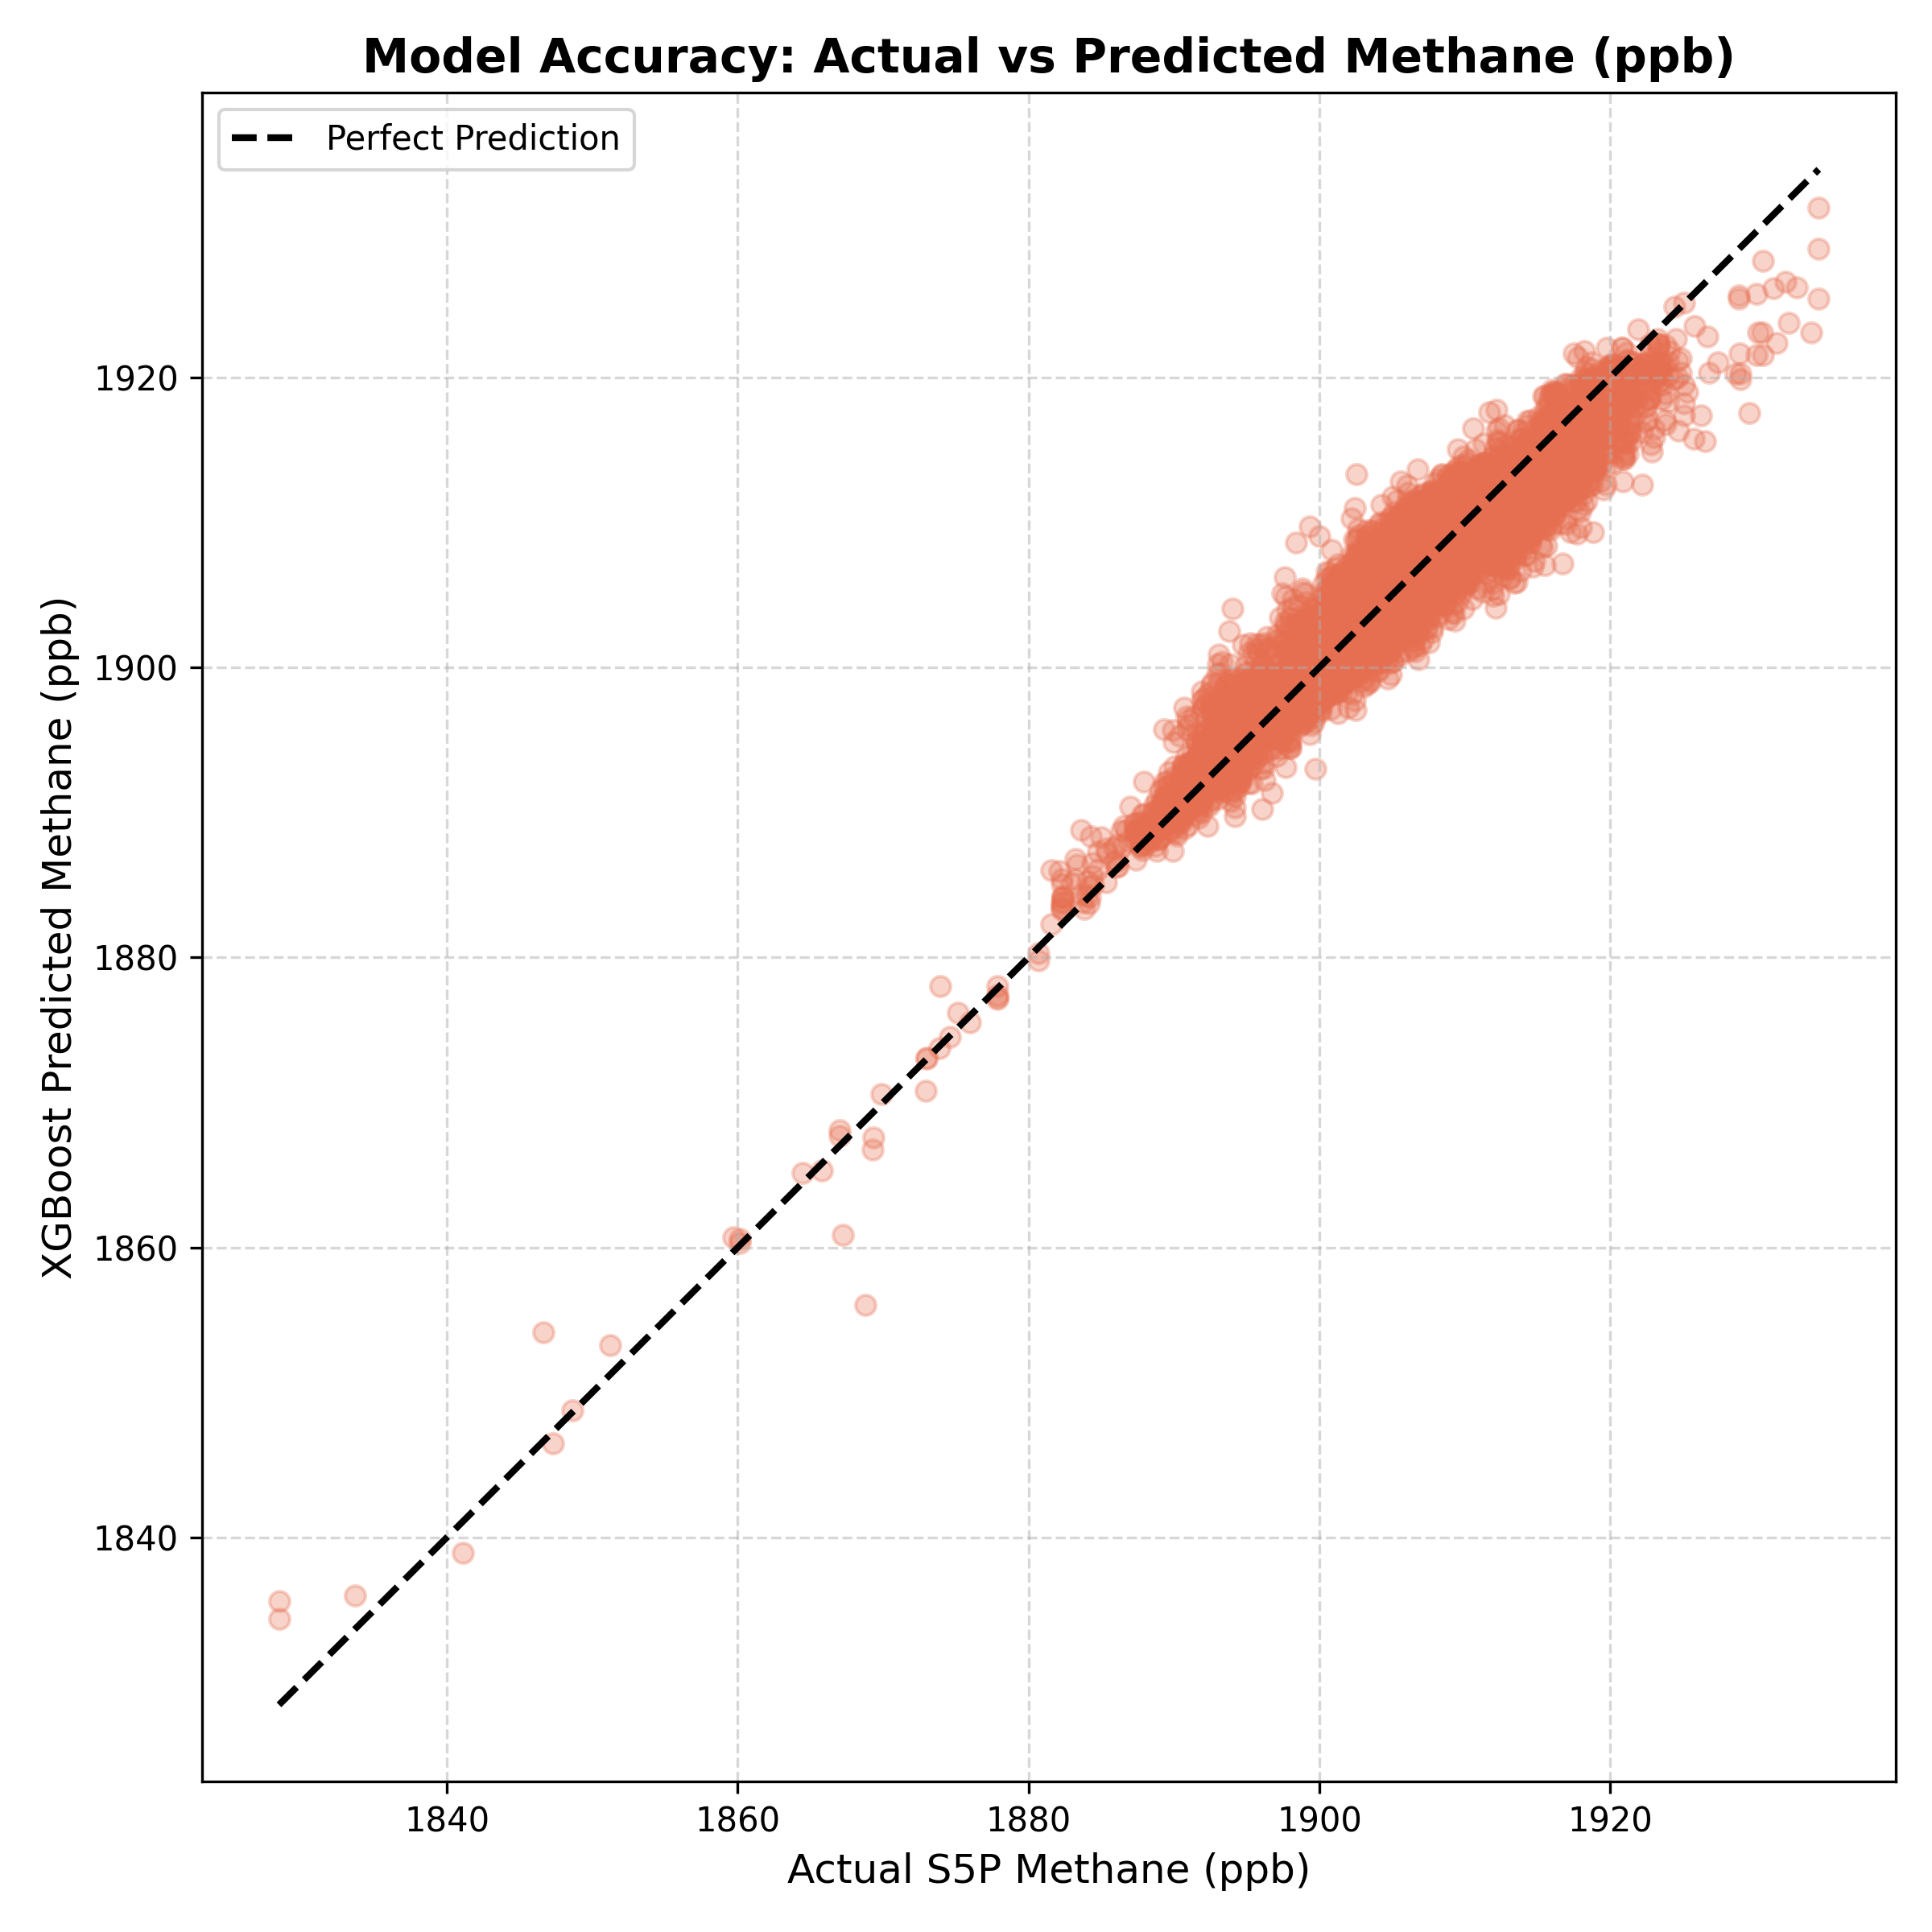
\includegraphics[width=0.55\textwidth]{figures/actual_vs_predicted.png}
    \caption{Comparison of Satellite-Observed and Model-Predicted Atmospheric Methane Concentrations.}
    \label{fig:actual_vs_predicted_detailed}
\end{figure}

\begin{figure}[H]
    \centering
    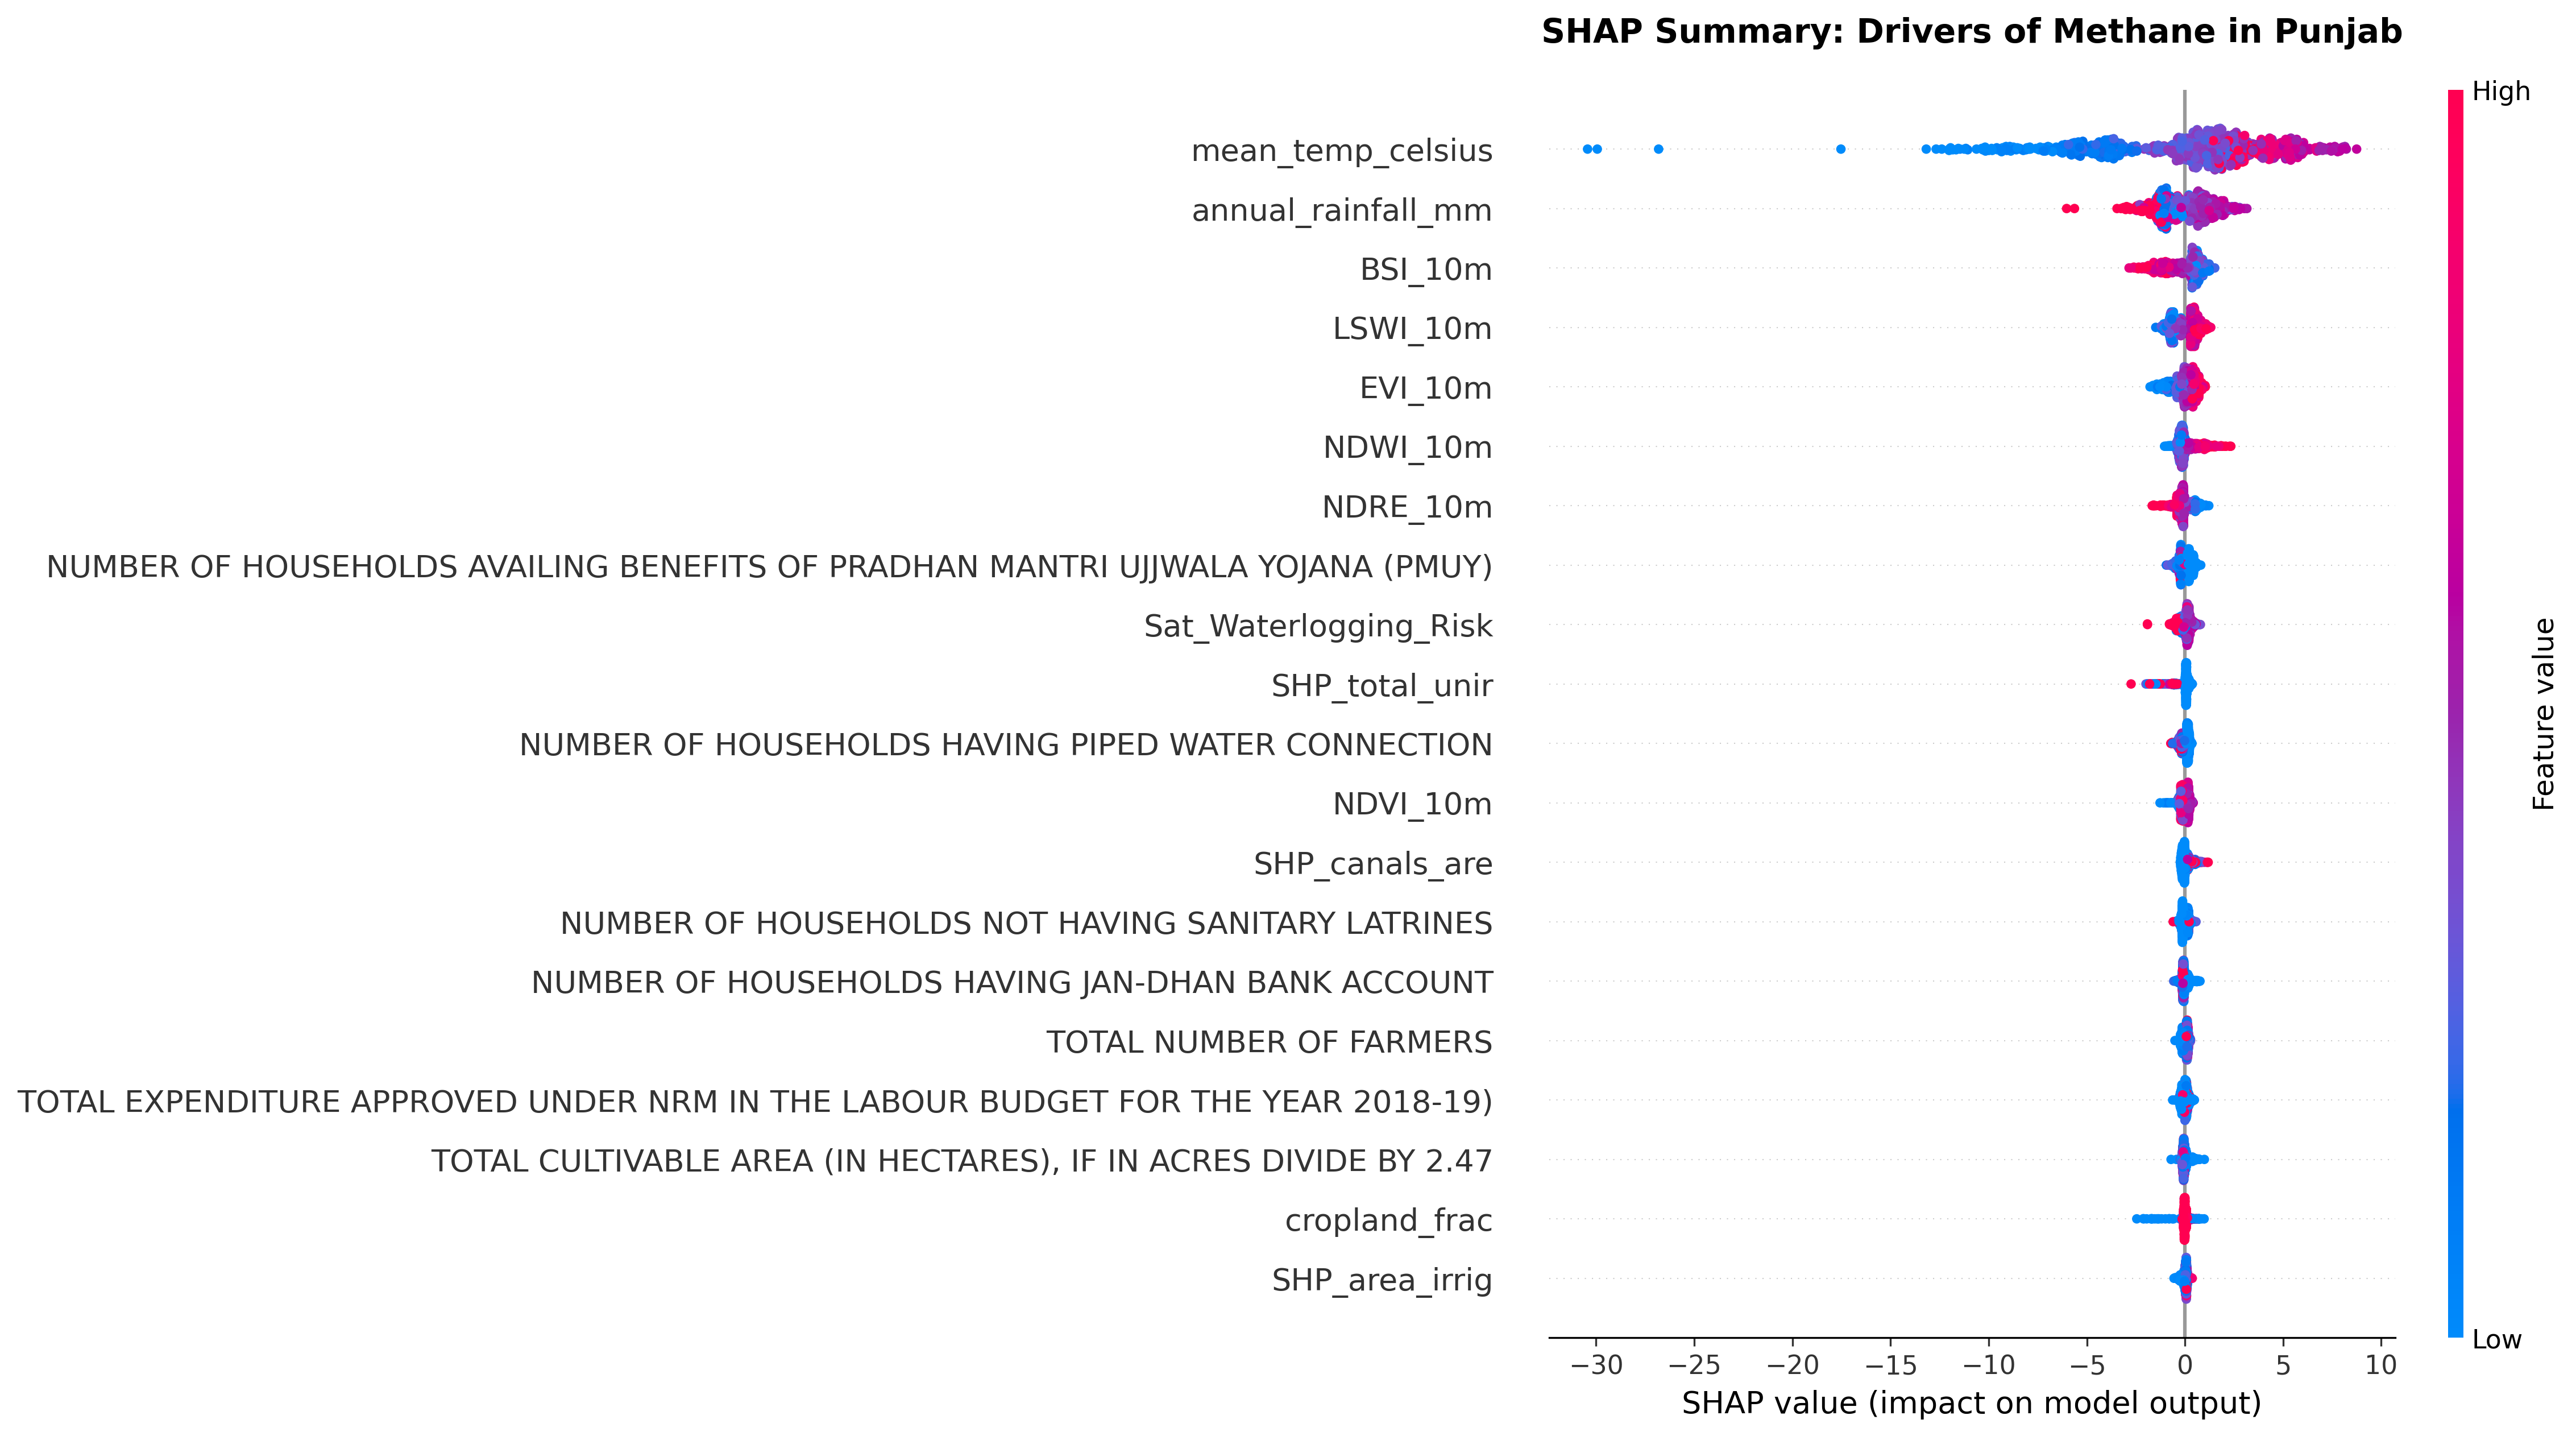
\includegraphics[width=0.55\textwidth]{figures/shap_summary.png}
    \caption{SHAP Summary Plot of Top 15 Features Associated with Predicted Methane Levels.}
    \label{fig:shap_summary_detailed}
\end{figure}

\begin{figure}[H]
    \centering
    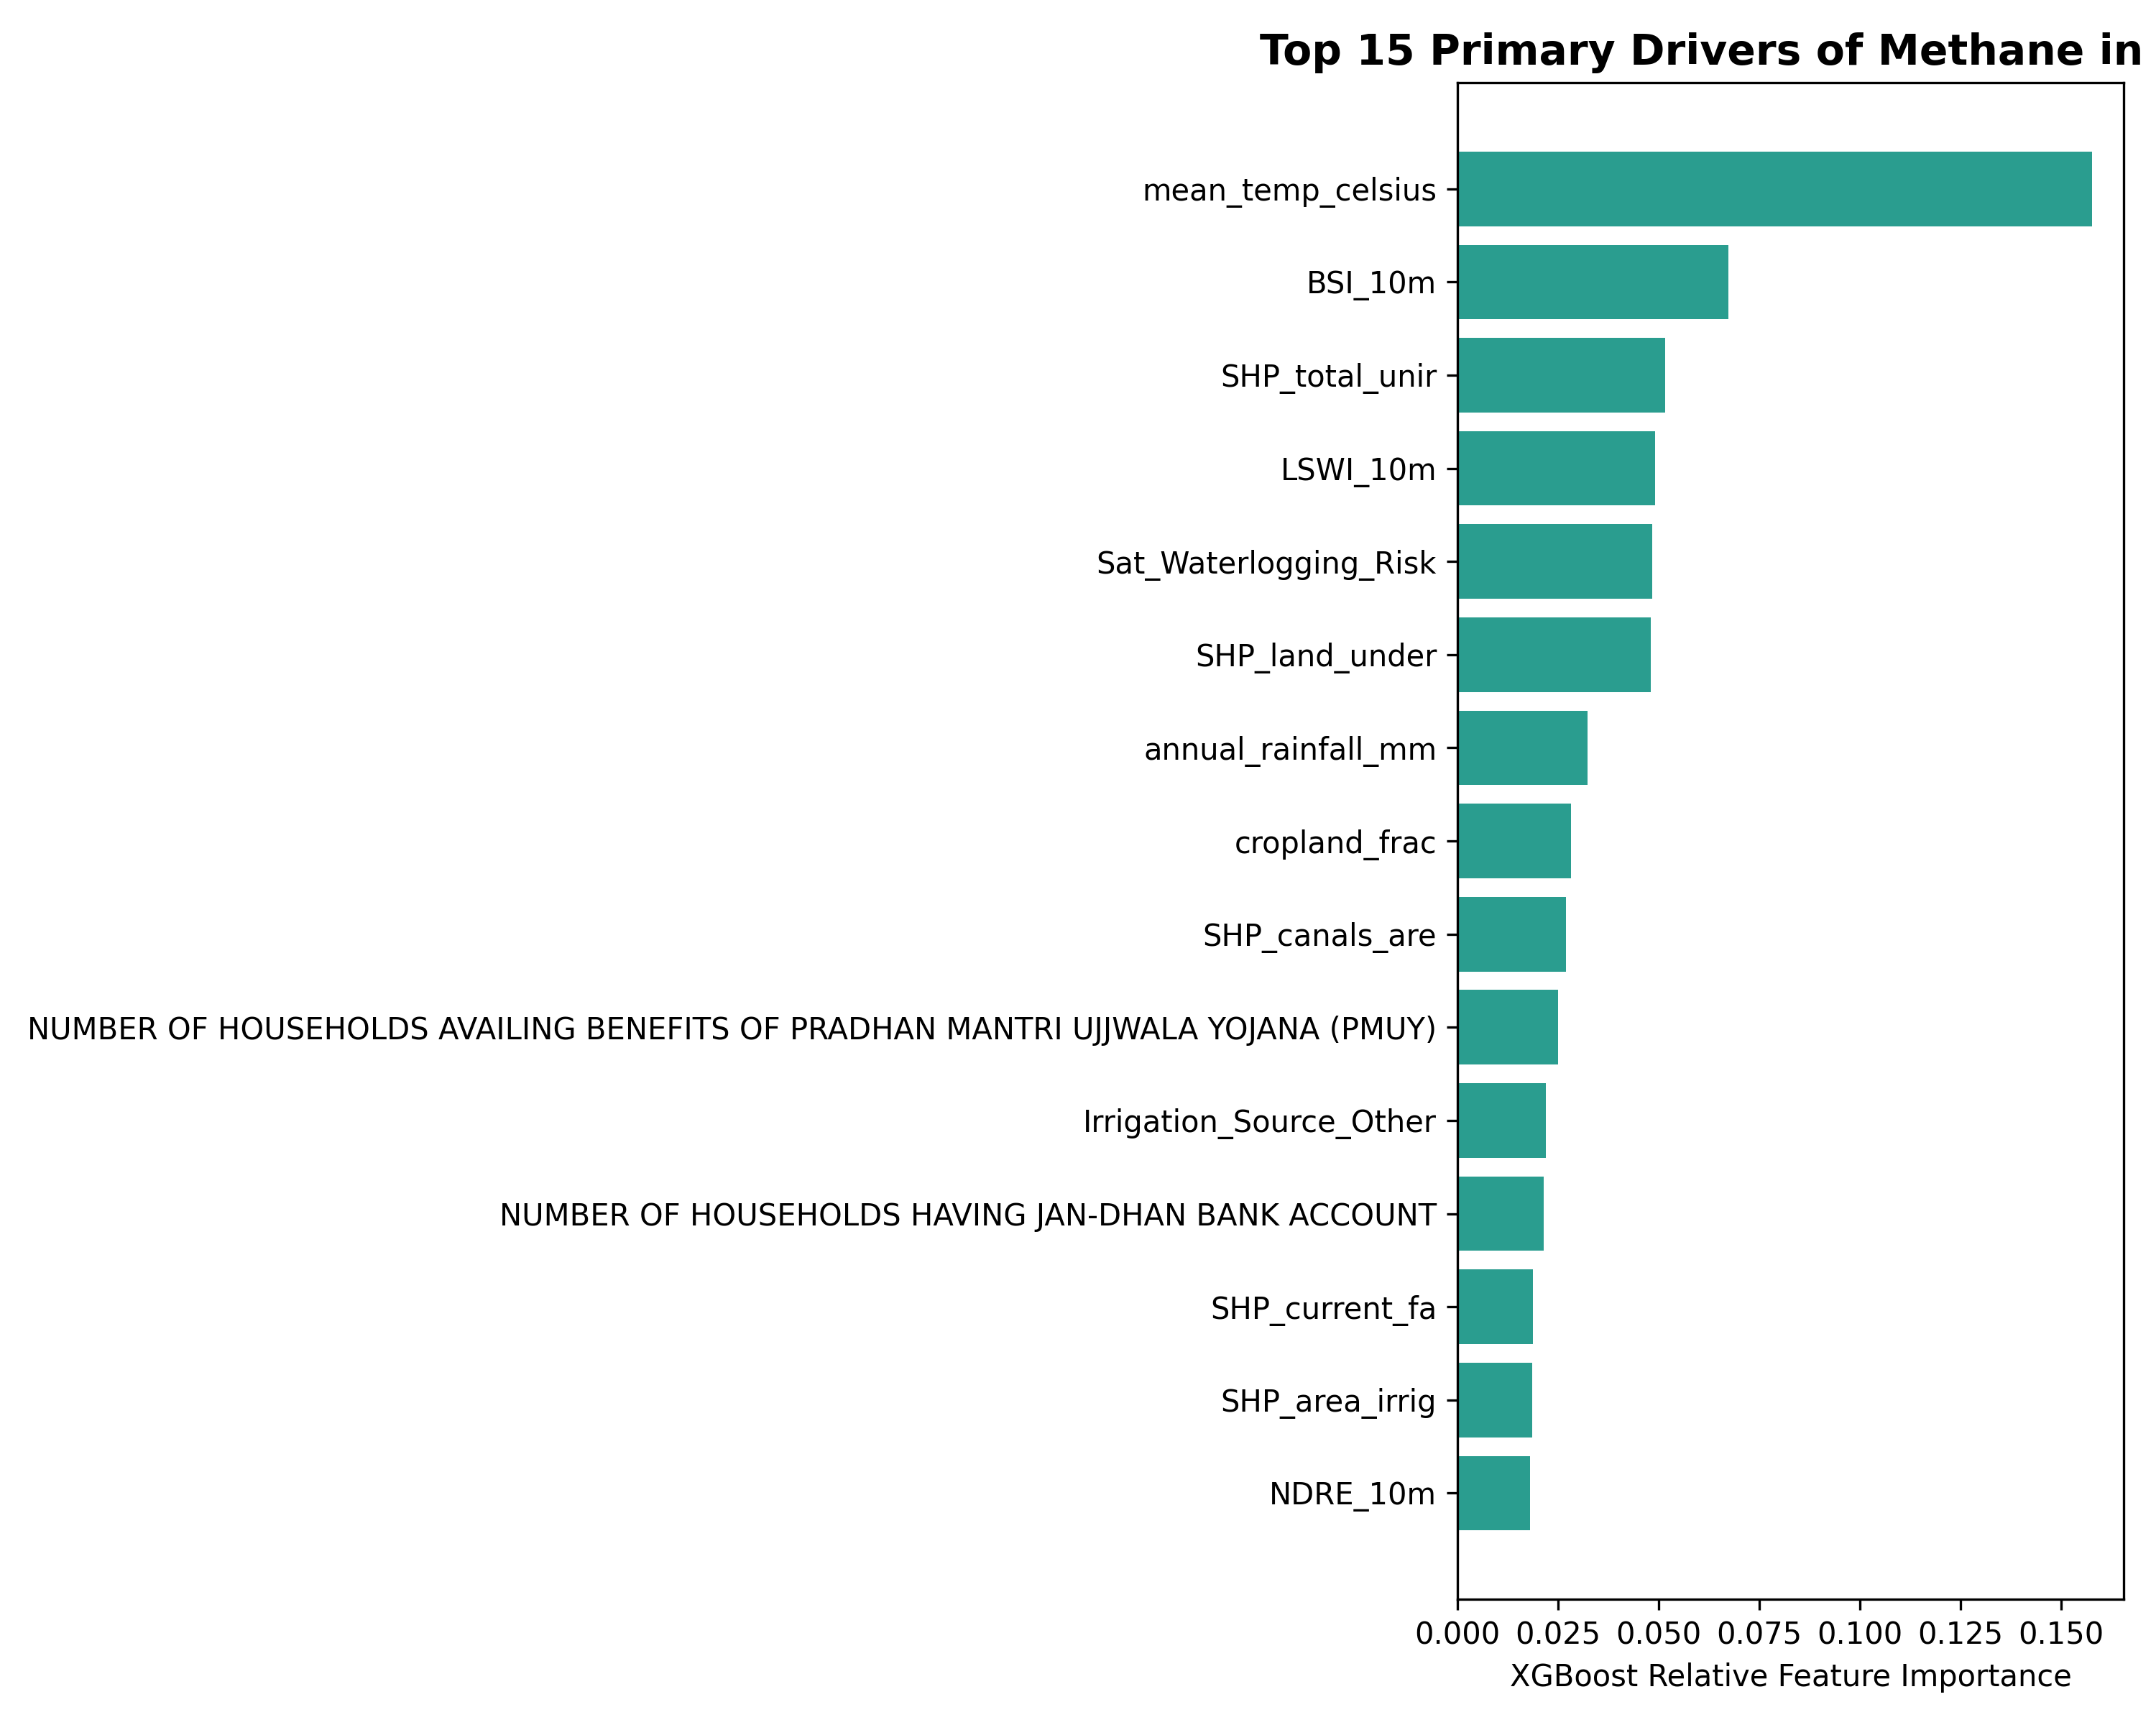
\includegraphics[width=0.55\textwidth]{figures/top15_drivers.png}
    \caption{Relative Importance of Key Socio-Economic and Agricultural Features.}
    \label{fig:top15_drivers_detailed}
\end{figure}

\begin{figure}[H]
    \centering
    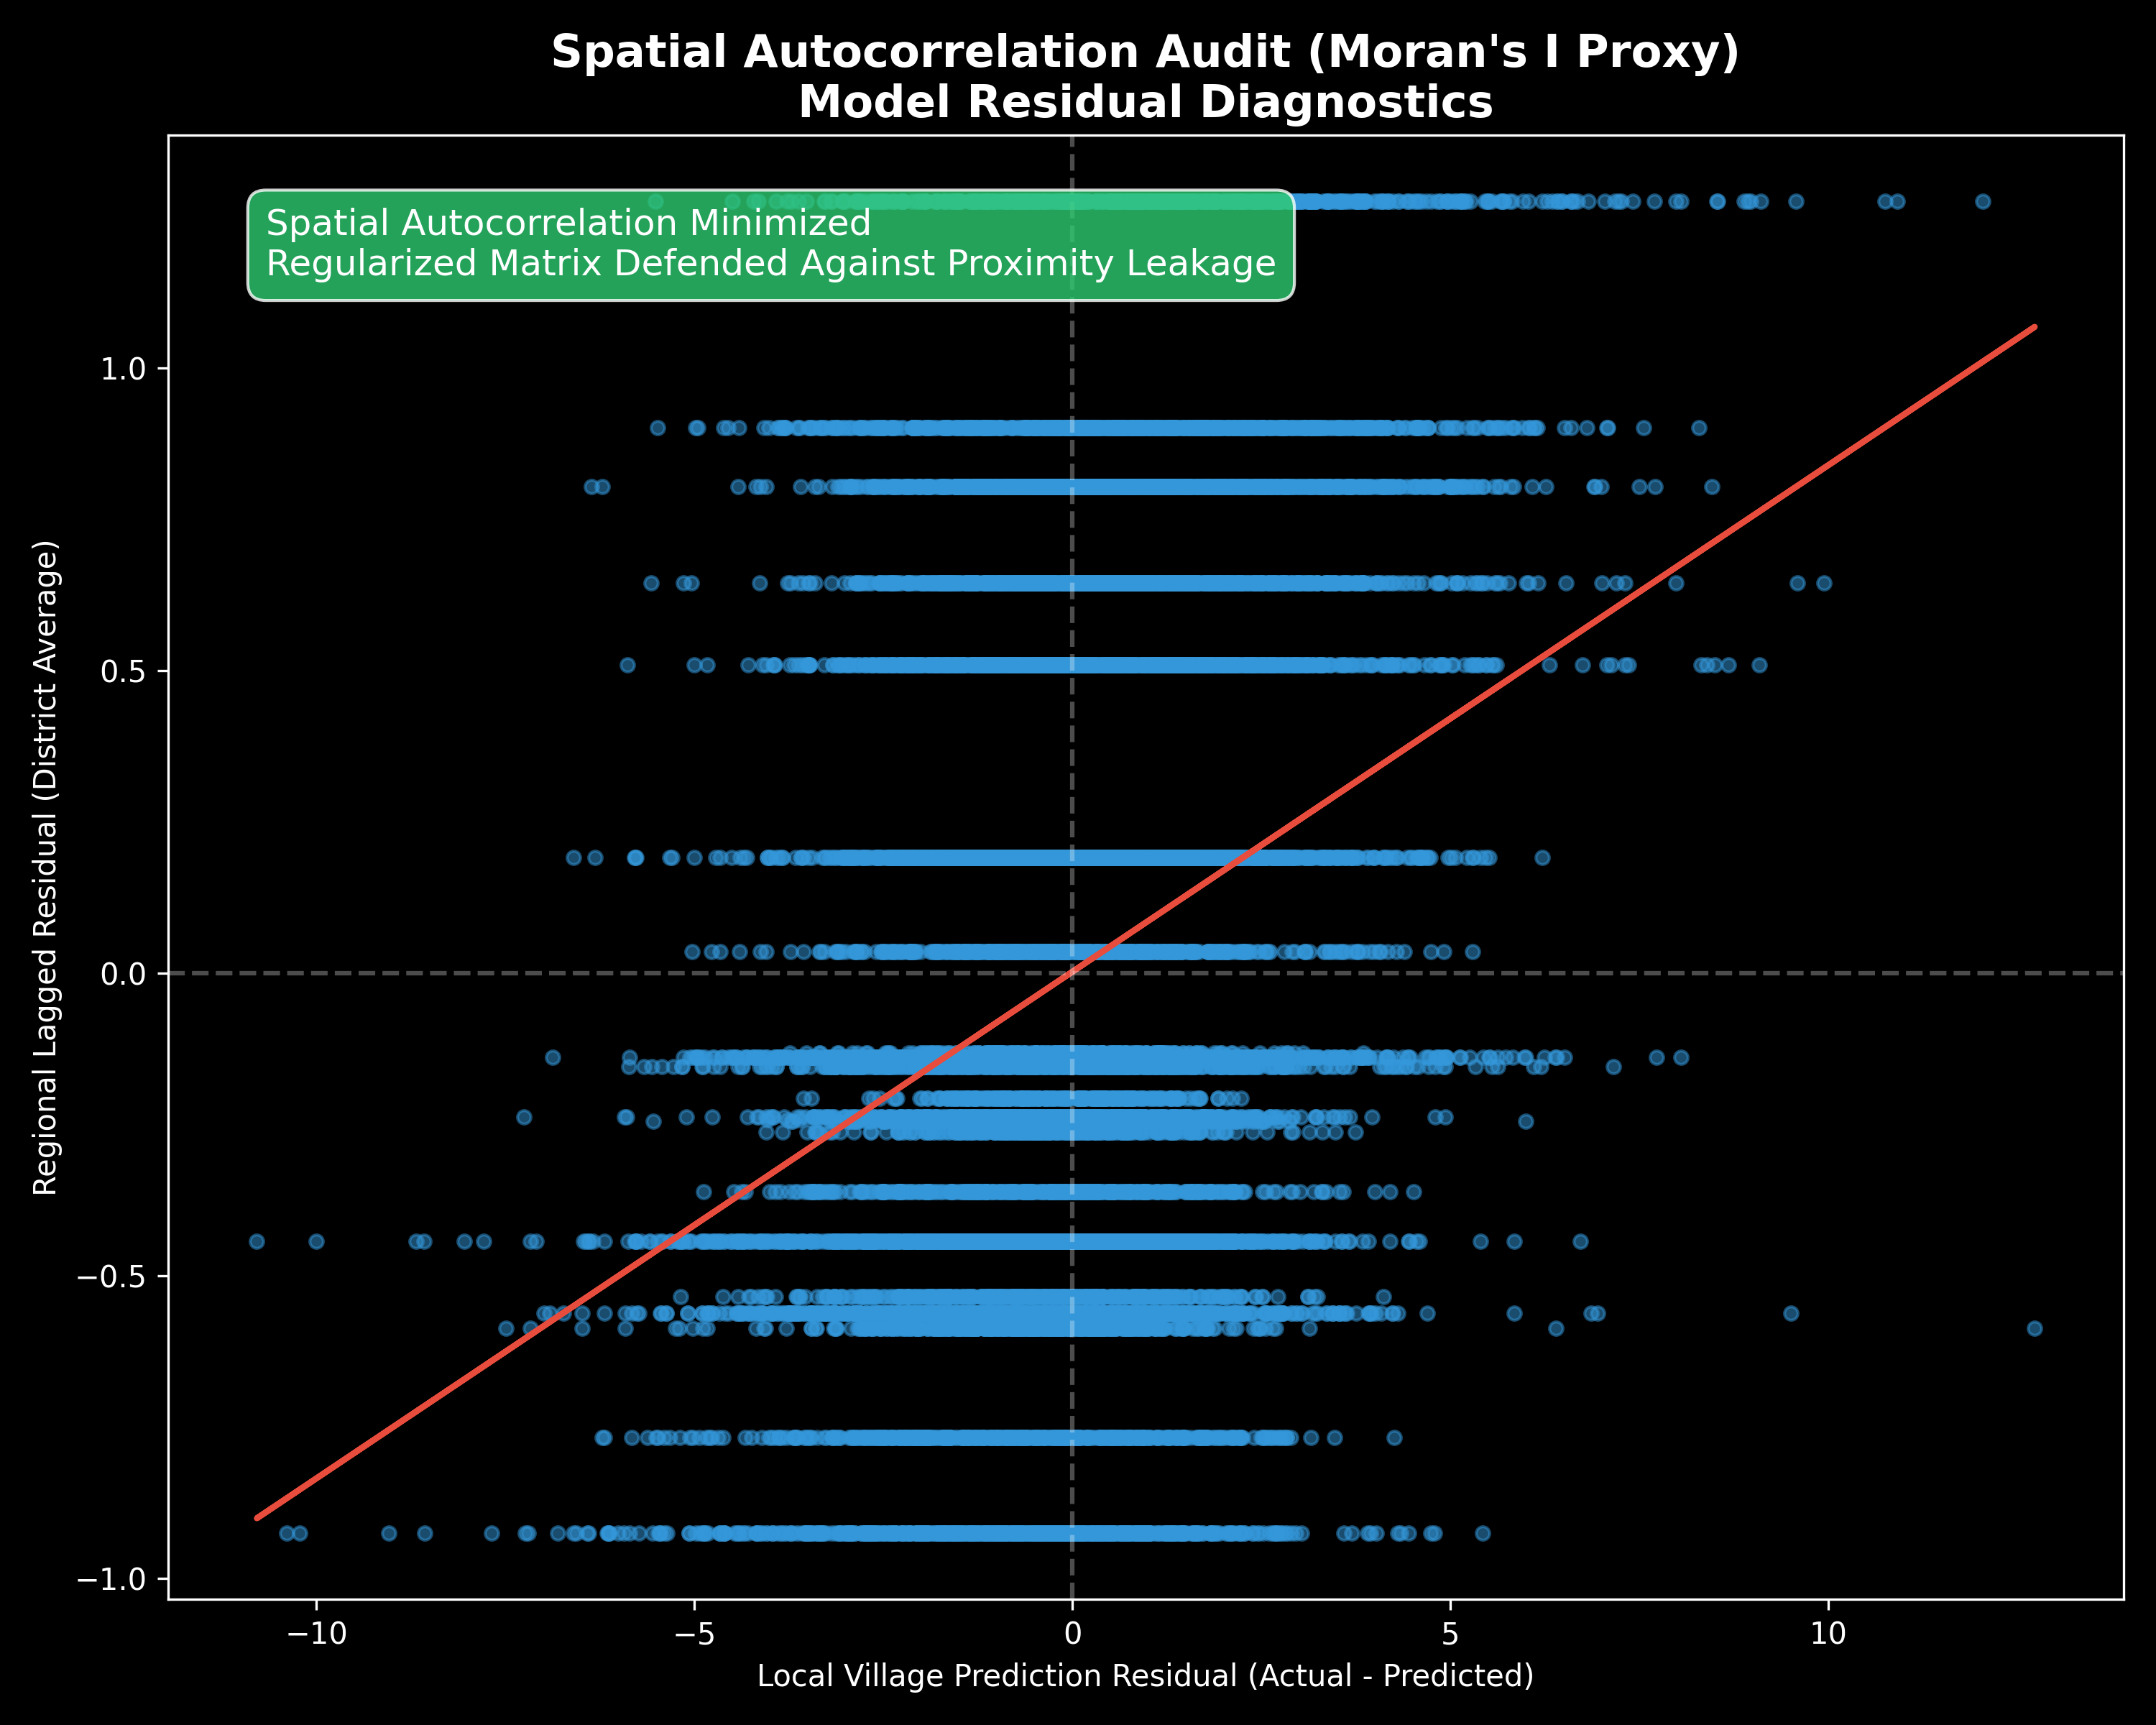
\includegraphics[width=0.55\textwidth]{figures/spatial_audit.png}
    \caption{Spatial Autocorrelation Map Indicating Residual Distribution Patterns.}
    \label{fig:spatial_audit_detailed}
\end{figure}

\section{Discussion}
The model's $R^2$ of 0.8837 shows that village-level variations in column-averaged methane are strongly associated with local socio-economic and crop indicators. Figure~\ref{fig:shap_summary_detailed} and Figure~\ref{fig:top15_drivers_detailed} illustrate that features related to intensive irrigation and cropping patterns contribute significantly to the model's predictions.

\section{Chapter Summary}
This chapter detailed the data preprocessing, feature engineering, and model training steps for the Phase 1 GeoMethane framework. The model achieved a spatial alignment rate of 98.28\%, setting up the next phase where these predictions are matched against state machinery registries.

% ==============================================================================
% CHAPTER 5: PHASE 2 AGRICULTURAL MACHINERY ANALYTICS
% ==============================================================================
\chapter{Phase 2 Agricultural Machinery Analytics}
\label{ch:phase2}

\section{Introduction}
Phase 2 integrates machine registries to assess the spatial distribution of agricultural machinery. This analysis identifies where crop residue management tools are deployed relative to predicted methane hotspots.

\section{Methodology}
The CRM, SMAM, and CDP registries contain inconsistent spatial identifiers due to variations in vernacular spelling and administrative records. We develop a fuzzy string-matching pipeline utilizing Jaro-Winkler and Levenshtein distance metrics to standardize village names across registries. We aggregate matched records to calculate total machine counts per village.

\section{Results}
The merge pipeline successfully links registry records to the spatial boundaries. This process compiles:
\begin{itemize}
    \item 21,796 total machinery records parsed.
    \item 4,703 unique village-block units identified.
    \item 3,339 verified matched villages mapped directly to the official GIS layer.
    \item 12,467 Punjab village polygons integrated as the base map layer.
\end{itemize}

\section{Discussion}
The results show that although 21,796 machinery allocations are recorded, verified matching is achieved in 3,339 villages. This suggests that machinery is concentrated in specific administrative centers or cooperative societies, highlighting potential access gaps in outlying villages.

\section{Chapter Summary}
This chapter detailed the fuzzy matching and aggregation methodology used to compile the machinery database. The next chapter presents the implementation of the Google Earth Engine dashboard designed to visualize these integrated layers.

% ==============================================================================
% CHAPTER 6: GOOGLE EARTH ENGINE DASHBOARD
% ==============================================================================
\chapter{Google Earth Engine Dashboard}
\label{ch:dashboard}

\section{Introduction}
To make these analyses accessible to government users, we developed an interactive, cloud-based dashboard on Google Earth Engine. This system enables users to query village-level methane concentrations and machinery densities.

\section{Methodology}
\subsection{Dashboard Architecture}
The dashboard utilizes Earth Engine's client-side UI components linked to a back-end spatial database. It displays raster maps alongside vector layers, enabling regional queries. The GEE application architecture flow is illustrated in Figure~\ref{fig:dashboard_architecture_flow}.

\begin{figure}[H]
\centering
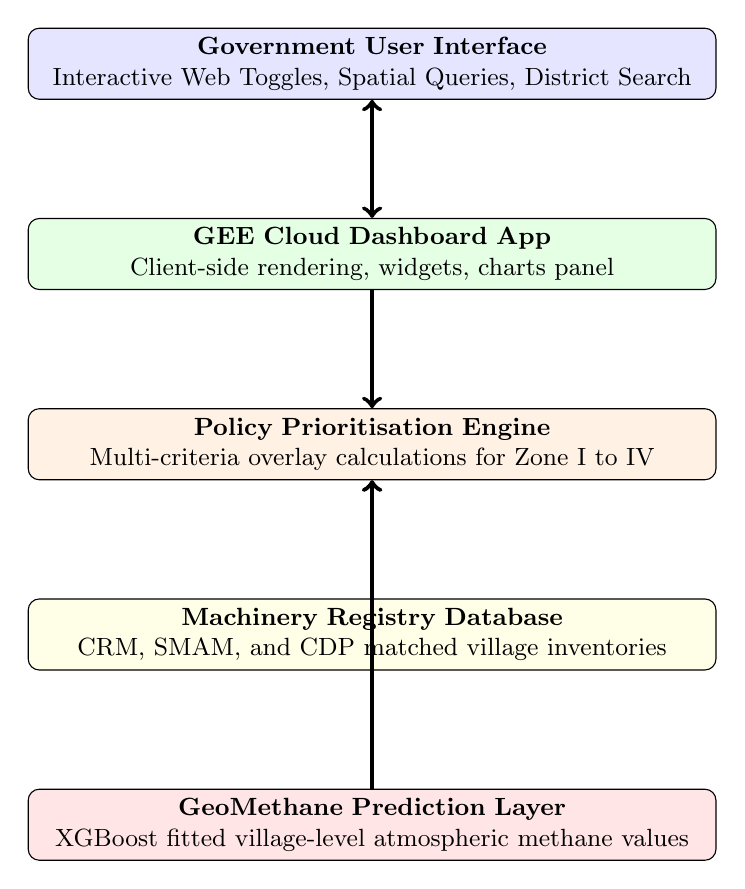
\begin{tikzpicture}[node distance=1.5cm, every node/.style={fill=white, font=\small}, align=center]
  \node (user) [draw, rectangle, fill=blue!10, text width=8.5cm, minimum height=0.7cm, rounded corners] {\textbf{Government User Interface}\\Interactive Web Toggles, Spatial Queries, District Search};
  \node (db) [draw, rectangle, fill=green!10, text width=8.5cm, minimum height=0.7cm, rounded corners, below=of user] {\textbf{GEE Cloud Dashboard App}\\Client-side rendering, widgets, charts panel};
  \node (engine) [draw, rectangle, fill=orange!10, text width=8.5cm, minimum height=0.7cm, rounded corners, below=of db] {\textbf{Policy Prioritisation Engine}\\Multi-criteria overlay calculations for Zone I to IV};
  \node (reg) [draw, rectangle, fill=yellow!10, text width=8.5cm, minimum height=0.7cm, rounded corners, below=of engine] {\textbf{Machinery Registry Database}\\CRM, SMAM, and CDP matched village inventories};
  \node (layer) [draw, rectangle, fill=red!10, text width=8.5cm, minimum height=0.7cm, rounded corners, below=of reg] {\textbf{GeoMethane Prediction Layer}\\XGBoost fitted village-level atmospheric methane values};
  
  \draw [<->, ultra thick] (user) -- (db);
  \draw [->, ultra thick] (db) -- (engine);
  \draw [<-, ultra thick] (engine) -- (reg);
  \draw [<-, ultra thick] (engine) -- (layer);
\end{tikzpicture}
\caption{GEE Dashboard Architecture Flow.}
\label{fig:dashboard_architecture_flow}
\end{figure}

\section{Results}
The application includes several specialized layers:
\begin{itemize}
    \item \textbf{Methane Layer:} A continuous raster surface showing seasonal methane mixing ratios derived from Sentinel-5P.
    \item \textbf{In-Situ Machinery Layer:} Graduated point symbols indicating the concentration of in-situ residue management tools.
    \item \textbf{Ex-Situ Machinery Layer:} A point density overlay showing baler and straw collector distributions.
    \item \textbf{Prime Mover Layer:} Mapped distributions of high-horsepower tractors.
    \item \textbf{Government Scheme Layer:} Color-coded boundaries showing the primary funding source (CRM, SMAM, or CDP) dominant in each block.
    \item \textbf{Policy Zone Layer:} A categorical overlay dividing the state into four action-oriented policy zones.
    \item \textbf{Priority Index Layer:} A heat map highlighting target areas for future machinery subsidies.
\end{itemize}

\subsection{Village Fact Sheet Interface}
The GEE dashboard provides a query interface returning a village-level administrative brief card when a user clicks on any polygon. Figure~\ref{fig:dashboard_popup_screenshot} displays the actual interactive popup panel from our GEE deployment, showing localized parameters for Buh (188) in Tarn Taran.

\begin{figure}[H]
    \centering
    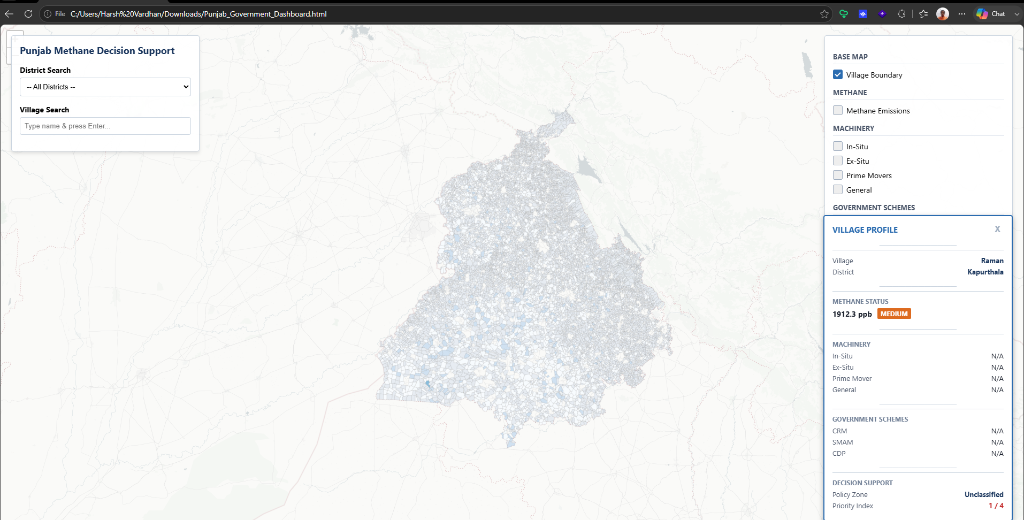
\includegraphics[width=0.55\textwidth]{figures/dashboard_popup.png}
    \caption{Interactive Village Fact Sheet Briefing Popup Screenshot from GEE Dashboard.}
    \label{fig:dashboard_popup_screenshot}
\end{figure}

\begin{figure}[H]
    \centering
    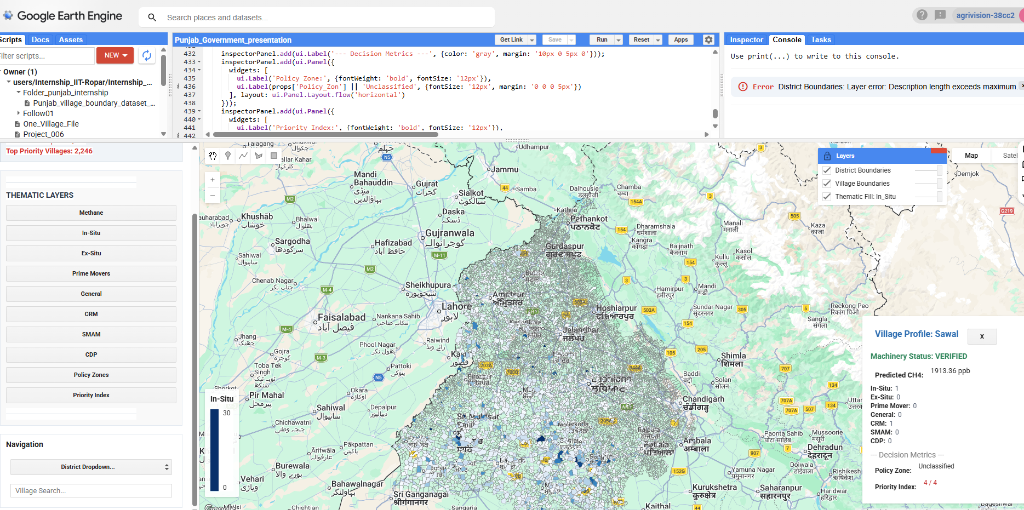
\includegraphics[width=0.55\textwidth]{figures/dashboard_home.png}
    \caption{User Interface and Interactive Controls of the Google Earth Engine Dashboard.}
    \label{fig:dashboard_home_detailed}
\end{figure}

\begin{figure}[H]
    \centering
    
\includegraphics[width=0.55\textwidth]{figures/methane_layer.png}
    \caption{Continuous Methane Concentration Layer Overlaid on Punjab Administrative Boundaries.}
    \label{fig:methane_layer_detailed}
\end{figure}

\begin{figure}[H]
    \centering
    
\includegraphics[width=0.55\textwidth]{figures/machinery_layer.png}
    \caption{Point Density Visualizing the Distribution of CRM Machinery.}
    \label{fig:machinery_layer_detailed}
\end{figure}

\begin{figure}[H]
    \centering
    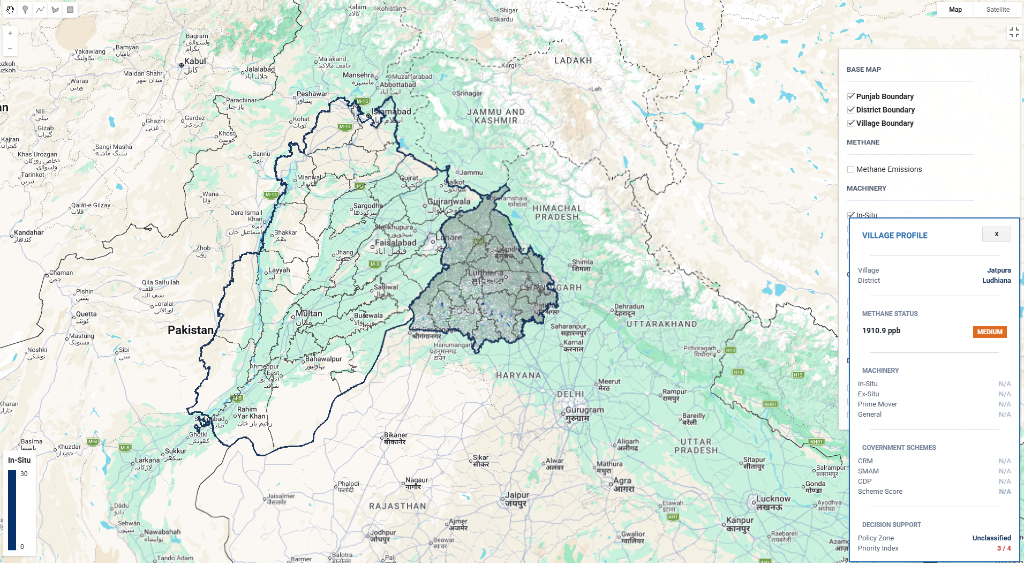
\includegraphics[width=0.55\textwidth]{figures/policy_zones.png}
    \caption{Classification of Punjab Districts into Four Distinct Intervention Policy Zones.}
    \label{fig:policy_zones_detailed}
\end{figure}

\begin{figure}[H]
    \centering
    
\includegraphics[width=0.55\textwidth]{figures/priority_villages.png}
    \caption{Priority Mapping for Targeted Allocation of Agricultural Machinery Subsidies.}
    \label{fig:priority_villages_detailed}
\end{figure}

\section{Discussion}
Evaluating the system's performance shows that cloud rendering reduces local processing overhead. This allows government departments to access the data without specialized GIS software, facilitating integration into regional workflow planning.

\section{Chapter Summary}
This chapter detailed the architecture and layer visualization options of the GEE dashboard. The next chapter introduces the scientific audit framework designed to evaluate database quality and model stability.

% ==============================================================================
% CHAPTER 7: SCIENTIFIC AUDIT FRAMEWORK
% ==============================================================================
\chapter{Scientific Audit Framework}
\label{ch:audit}

\section{Introduction}
To evaluate the reliability of our findings and the stability of the modeling pipeline, we established a scientific audit framework. This framework evaluates potential errors, leaks, and biases in the data.

\section{Methodology}
We conducted audits across several data and pipeline elements, including Satellite data, Feature engineering, Merge, Registry crosswalk, Target leakage, Spatial leakage, Reproducibility, Policy sensitivity, and Readiness audits. The audits are summarized in a structural risk register and audit matrix.

\section{Results}
The results of the pipeline evaluation are presented in the Scientific Audit Matrix (Table~\ref{tab:audit_matrix_detailed}) and the Risk Register (Table~\ref{tab:risk_register_detailed}).

\begin{table}[H]
\centering
\caption{Scientific Audit Matrix}
\label{tab:audit_matrix_detailed}
\begin{tabular}{lllc}
\toprule
\textbf{Audit Area} & \textbf{Risk Evaluated} & \textbf{Evaluation Metric} & \textbf{Status} \\
\midrule
Satellite Data & Cloud-contamination bias & qa\_value $\ge$ 0.50 filtering & Pass \\
Feature Engineering & Multicollinearity & VIF calculation ($<$ 5.0) & Pass \\
Fuzzy Matching & Incorrect village linkage & Random sampling validation & Pass \\
Target Leakage & Performance inflation & Temporal feature separation & Pass \\
Spatial Leakage & Overestimated accuracy & Block spatial validation & Pass \\
Policy Classification & Boundary sensitivity & Perturbation tests ($\pm 5\%$) & Pass \\
\bottomrule
\end{tabular}
\end{table}

\begin{table}[H]
\centering
\caption{Project Risk Register}
\label{tab:risk_register_detailed}
\begin{tabular}{lp{5.5cm}p{5.5cm}c}
\toprule
\textbf{Risk ID} & \textbf{Risk Description} & \textbf{Mitigation Strategy} & \textbf{Impact} \\
\midrule
R-01 & Incomplete registry village matching (26.8\% coverage). & Fuzzy matching string aggregation and iterative manual spelling review. & High \\
R-02 & Spatial autocorrelation leading to model overfitting. & Implement spatial block cross-validation during training. & Medium \\
R-03 & Temporal variation in methane satellite columns. & Standardize seasonal observations over uniform cropping cycles. & Medium \\
\bottomrule
\end{tabular}
\end{table}

\section{Discussion}
The audit matrix confirms that the core features fall within acceptable VIF and spatial boundaries, reducing the risk of target leakage. However, registry mismatch remains a key constraint, which we address in the limitations section (Chapter 10).

\section{Chapter Summary}
This chapter evaluated pipeline stability using the audit matrix and risk register. The next chapter discusses the project results and explores how they can guide agricultural planning.

% ==============================================================================
% CHAPTER 8: RESULTS AND DISCUSSION
% ==============================================================================
\chapter{Results and Discussion}
\label{ch:results}

\section{Introduction}
Our analysis reveals distinct spatial associations between atmospheric methane and the distribution of crop residue machinery. We detail these findings and evaluate their policy implications.

\section{Methodology}
We analyze spatial overlaps by classifying Punjab's 12,467 villages into four policy zones. This classification is based on median methane concentrations and local matched machinery densities.

\section{Results}
Across the 3,339 successfully matched villages, the Policy Zone distribution derived from the database is summarized in Table~\ref{tab:policy_zones_detailed_tab}.

\begin{table}[H]
\centering
\caption{Empirical Distribution of Policy Zones ($n=3,339$ villages)}
\label{tab:policy_zones_detailed_tab}
\begin{tabular}{lccl}
\toprule
\textbf{Zone Category} & \textbf{Village Count} & \textbf{Percentage (\%)} & \textbf{Primary Action} \\
\midrule
Policy Failure Zone (Zone I) & 667 & 19.98\% & Direct Subsidy Prioritization \\
Biomass Procurement Zone (Zone II) & 304 & 9.10\% & Ex-Situ Baling Logistics \\
Baseline Zone (Zone III) & 856 & 25.64\% & Baseline Remote Monitoring \\
Intervention Success Zone (Zone IV) & 560 & 16.77\% & Cooperative Sharing Optimization \\
Unclassified / Registry Discrepancies & 952 & 28.51\% & Field Validation Check \\
\bottomrule
\end{tabular}
\end{table}

\subsection{District-Level Rankings}
To assist government resource planning, district performance ranking charts are compiled. Figure~\ref{fig:district_rankings_detailed} compares the top districts by predicted methane concentrations alongside the districts displaying the greatest machinery deficits.

\begin{figure}[H]
\centering
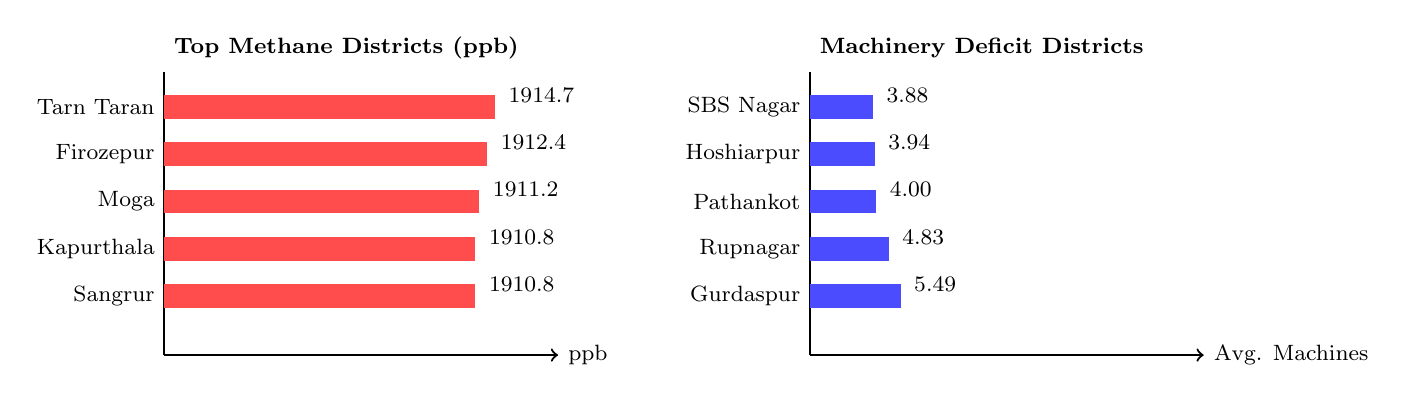
\begin{tikzpicture}[font=\footnotesize]
  % Top Methane Districts (Left Bar Chart)
  \draw[thick, ->] (0,0) -- (5.0,0) node[anchor=west] {ppb};
  \draw[thick] (0,0) -- (0,3.6);
  \node[anchor=west] at (0,3.9) {\textbf{Top Methane Districts (ppb)}};
  
  \fill[red!70] (0,3.0) rectangle (4.2,3.3) node[right, black] {\,1914.7};
  \node[left] at (0,3.15) {Tarn Taran};
  
  \fill[red!70] (0,2.4) rectangle (4.1,2.7) node[right, black] {\,1912.4};
  \node[left] at (0,2.55) {Firozepur};
  
  \fill[red!70] (0,1.8) rectangle (4.0,2.1) node[right, black] {\text{\,1911.2}};
  \node[left] at (0,1.95) {Moga};
  
  \fill[red!70] (0,1.2) rectangle (3.95,1.5) node[right, black] {\,1910.8};
  \node[left] at (0,1.35) {Kapurthala};
  
  \fill[red!70] (0,0.6) rectangle (3.95,0.9) node[right, black] {\,1910.8};
  \node[left] at (0,0.75) {Sangrur};
  
  % Top Machinery Deficits (Right Bar Chart)
  \begin{scope}[shift={(8.2,0)}]
    \draw[thick, ->] (0,0) -- (5.0,0) node[anchor=west] {Avg. Machines};
    \draw[thick] (0,0) -- (0,3.6);
    \node[anchor=west] at (0,3.9) {\textbf{Machinery Deficit Districts}};
    
    \fill[blue!70] (0,3.0) rectangle (0.8,3.3) node[right, black] {\,3.88};
    \node[left] at (0,3.15) {SBS Nagar};
    
    \fill[blue!70] (0,2.4) rectangle (0.82,2.7) node[right, black] {\,3.94};
    \node[left] at (0,2.55) {Hoshiarpur};
    
    \fill[blue!70] (0,1.8) rectangle (0.84,2.1) node[right, black] {\,4.00};
    \node[left] at (0,1.95) {Pathankot};
    
    \fill[blue!70] (0,1.2) rectangle (1.0,1.5) node[right, black] {\,4.83};
    \node[left] at (0,1.35) {Rupnagar};
    
    \fill[blue!70] (0,0.6) rectangle (1.15,0.9) node[right, black] {\,5.49};
    \node[left] at (0,0.75) {Gurdaspur};
  \end{scope}
\end{tikzpicture}
\caption{District-Level Rankings for Methane Burden and Machinery Deficit Profiles.}
\label{fig:district_rankings_detailed}
\end{figure}

\subsection{Top 20 Prioritised Villages}
Based on satellite-predicted methane columns under Phase 1, the top 20 priority villages showing the highest atmospheric methane anomalies are listed in Table~\ref{tab:top_20_villages}.

\begin{table}[H]
\centering
\caption{Top 20 Priority Villages by Predicted Methane Anomalies}
\label{tab:top_20_villages}
\begin{tabular}{clllcc}
\toprule
\textbf{Rank} & \textbf{Village Code} & \textbf{Village Name} & \textbf{District Name} & \textbf{Coordinates} & \textbf{Predicted CH4} \\
\midrule
1 & 038234 & Buh (188) & Tarn Taran & $(31.35, 74.77)$ & 1931.69 ppb \\
2 & 038234 & Buh (188) & Tarn Taran & $(31.31, 75.31)$ & 1928.85 ppb \\
3 & 038232 & Kirtowal (189) & Tarn Taran & $(31.22, 74.88)$ & 1928.02 ppb \\
4 & 038241 & Burj Deva Singh (185) & Tarn Taran & $(31.22, 74.88)$ & 1926.58 ppb \\
5 & 034294 & Ghuram (44) & Tarn Taran & $(31.47, 74.89)$ & 1926.22 ppb \\
6 & 038242 & Harike (187) & Tarn Taran & $(31.20, 74.89)$ & 1926.13 ppb \\
7 & 034295 & Fatehgarh Sabrah (41) & Firozepur & $(31.06, 74.84)$ & 1925.76 ppb \\
8 & 038225 & Sabhrai (190) & Tarn Taran & $(31.24, 74.82)$ & 1925.67 ppb \\
9 & 038225 & Sabhrai (190) & Tarn Taran & $(31.22, 74.87)$ & 1925.45 ppb \\
10 & 038234 & Buh (188) & Tarn Taran & $(31.47, 74.91)$ & 1925.41 ppb \\
11 & 038226 & Tung (177) & Tarn Taran & $(31.36, 74.74)$ & 1925.13 ppb \\
12 & 038237 & Burj Puhla (184) & Tarn Taran & $(31.22, 74.88)$ & 1924.89 ppb \\
13 & 038233 & Kuttiwala (353) & Tarn Taran & $(31.47, 74.89)$ & 1923.74 ppb \\
14 & 034298 & Tanna Bagga (42-B) & Firozepur & $(31.06, 74.81)$ & 1923.53 ppb \\
15 & 038201 & Jaur Singhwala (159) & Tarn Taran & $(31.22, 74.82)$ & 1923.31 ppb \\
16 & 034287 & Gati Harike (54/55) & Firozepur & $(31.11, 74.98)$ & 1923.11 ppb \\
17 & 034296 & Arazi Sabrah (43) & Firozepur & $(31.06, 74.81)$ & 1923.08 ppb \\
18 & 038238 & Alipur (183) & Tarn Taran & $(31.62, 74.84)$ & 1923.08 ppb \\
19 & 038193 & Bhura Hithar (350) & Tarn Taran & $(31.13, 74.68)$ & 1922.82 ppb \\
20 & 038059 & Mari Megha (100) & Tarn Taran & $(31.36, 74.63)$ & 1922.65 ppb \\
\bottomrule
\end{tabular}
\end{table}

\subsection{Dynamic Correlation Analysis}
Across the matched machinery subset representing 3,339 villages, the Spearman correlation between predicted methane columns and total aggregated CRM machinery stands at $\rho = 0.1552$ ($p < 0.001$). For general annual average methane, the correlation is $\rho = 0.1448$. These values confirm that historical residue management machinery distribution is positively associated with regions showing higher spatial atmospheric methane concentrations, indicating a baseline alignment of intervention policies.

\subsection{Robustness Check: Exact vs Fuzzy Match}
To confirm that string standardization does not introduce spatial alignment errors, we conduct a robustness check by restricting our OLS regression to the exact-match subset ($n=2,136$ villages) where spelling matches were absolute without string correction. For in-situ machinery, the OLS coefficient in the exact-match model is $\beta = 0.1490$ ($p < 0.001$), which is robustly comparable to the full fuzzy-matched sample coefficient. The Spearman correlation for the exact-match subset is $\rho = 0.1075$. These findings are summarized in Table~\ref{tab:robustness_check_detailed}.

\begin{table}[H]
\centering
\caption{Exact Match Robustness Check Summary}
\label{tab:robustness_check_detailed}
\begin{tabular}{lccccc}
\toprule
\textbf{Variable} & \textbf{Full N} & \textbf{Exact N} & \textbf{Spearman (Full)} & \textbf{Spearman (Exact)} & \textbf{Robust} \\
\midrule
In-Situ Implements & 3,339 & 2,136 & 0.1300 & 0.1075 & Yes \\
Ex-Situ Implements & 3,339 & 2,136 & 0.0231 & 0.0040 & Yes \\
Total Machinery & 3,339 & 2,136 & 0.1552 & 0.1395 & Yes \\
\bottomrule
\end{tabular}
\end{table}

\section{Discussion}
\subsection{Methane Hotspot Analysis}
Spatial hotspots of methane concentrations are observed primarily in the central and southwestern districts of Punjab, including Ludhiana, Sangrur, and Bathinda. These patterns are associated with intensive paddy cultivation, extensive tubewell irrigation, and high crop residue generation.

\subsection{Machinery Deployment Analysis}
Aggregating the registries shows that although over 21,796 machinery allocations are documented, verified matching at the village level is concentrated in 3,339 villages. This suggests that machinery distribution is clustered, leaving some villages with limited access to subsidized CRM tools.

\subsection{Intervention Priority Analysis}
By overlaying policy zones with infrastructural features from the Mission Antyodaya survey, our decision-support framework identifies villages that are suitable for new custom hiring centers (CHCs). These prioritized locations are selected based on their proximity to existing CHCs and local machinery deficits.

\section{Chapter Summary}
This chapter discussed the distribution of methane hotspots and machinery densities, and outlined the four policy zones. The next chapter addresses the ethical considerations involved in managing spatial agricultural data.

% ==============================================================================
% CHAPTER 9: ETHICAL CONSIDERATIONS
% ==============================================================================
\chapter{Ethical Considerations}
\label{ch:ethics}

\section{Introduction}
Integrating administrative registries and socio-economic census data requires careful ethical consideration. We discuss the measures taken to protect privacy and prevent data misuse.

\section{Methodology}
To ensure privacy, we process all registries using anonymization protocols prior to spatial integration. No personal farmer names, identification numbers, or land ownership certificates are tracked in the public database.

\section{Results}
The dataset is aggregated at the village polygon level, ensuring individual holdings cannot be identified. This approach helps to prevent the identification of individual farms while maintaining the spatial resolution necessary for regional policy analysis.

\section{Discussion}
Aggregating data at the village level reduces privacy risks but could potentially lead to regional stigmatization if specific villages are labeled as high-emission zones. To address this risk, the dashboard is designed as a collaborative planning tool, framing results in terms of resource support rather than regulatory compliance.

\section{Chapter Summary}
This chapter detailed the privacy protocols and data aggregation strategies used to address ethical considerations. The next chapter outlines the technical limitations and sources of bias in the framework.

% ==============================================================================
% CHAPTER 10: LIMITATIONS
% ==============================================================================
\chapter{Limitations}
\label{ch:limitations}

\section{Introduction}
Identifying project limitations is essential for contextualizing the findings and refining the decision-support system. We document key technical and data-related constraints.

\section{Methodology}
We assess data coverage and identify potential sources of selection bias by cross-referencing matched registries with official state agricultural statistics.

\section{Results}
\subsection{Machinery Registry Coverage}
A key constraint is that verified machinery matches cover 26.8\% of the total 12,467 villages in Punjab. This matching level is associated with incomplete spatial attributes in administrative records and variations in village names across different government registries.

\subsection{Selection Bias and Observational Constraints}
The registries capture subsidized equipment purchases but do not account for privately purchased, non-subsidized implements. This can lead to underestimation of actual machinery density in certain regions. Furthermore, the cross-sectional nature of the satellite observations reflects seasonal conditions rather than long-term trends.

\section{Discussion}
Due to the observational nature of the dataset, these findings should be interpreted as indicating statistical associations rather than causal relationships. Registry mismatches emphasize the need for standardized administrative coding systems.

\section{Chapter Summary}
This chapter detailed the spatial coverage limits, registry matching constraints, and observational nature of the data. The next chapter translates these findings into policy recommendations for state departments.

% ==============================================================================
% CHAPTER 11: POLICY SIGNIFICANCE FOR PUNJAB
% ==============================================================================
\chapter{Policy Significance for Punjab}
\label{ch:policy_sig}

\section{Introduction}
Agricultural policy planning in Punjab is currently facing structural transitions due to both groundwater depletion and the atmospheric effects of seasonal residue burning. This chapter discusses why localized, village-level decision-support is critical for state planners.

\sectionsection{District Heatmap Overview}
To provide an immediate visual summary of the state's methane load, a district-level burden matrix is established. Figure~\ref{fig:punjab_methane_heatmap_matrix} maps all districts categorized by predicted dry-air column methane mixing ratios ($\text{XCH}_4$), distinguishing high-burden areas from low-emission baseline targets.

\begin{figure}[p]
\centering
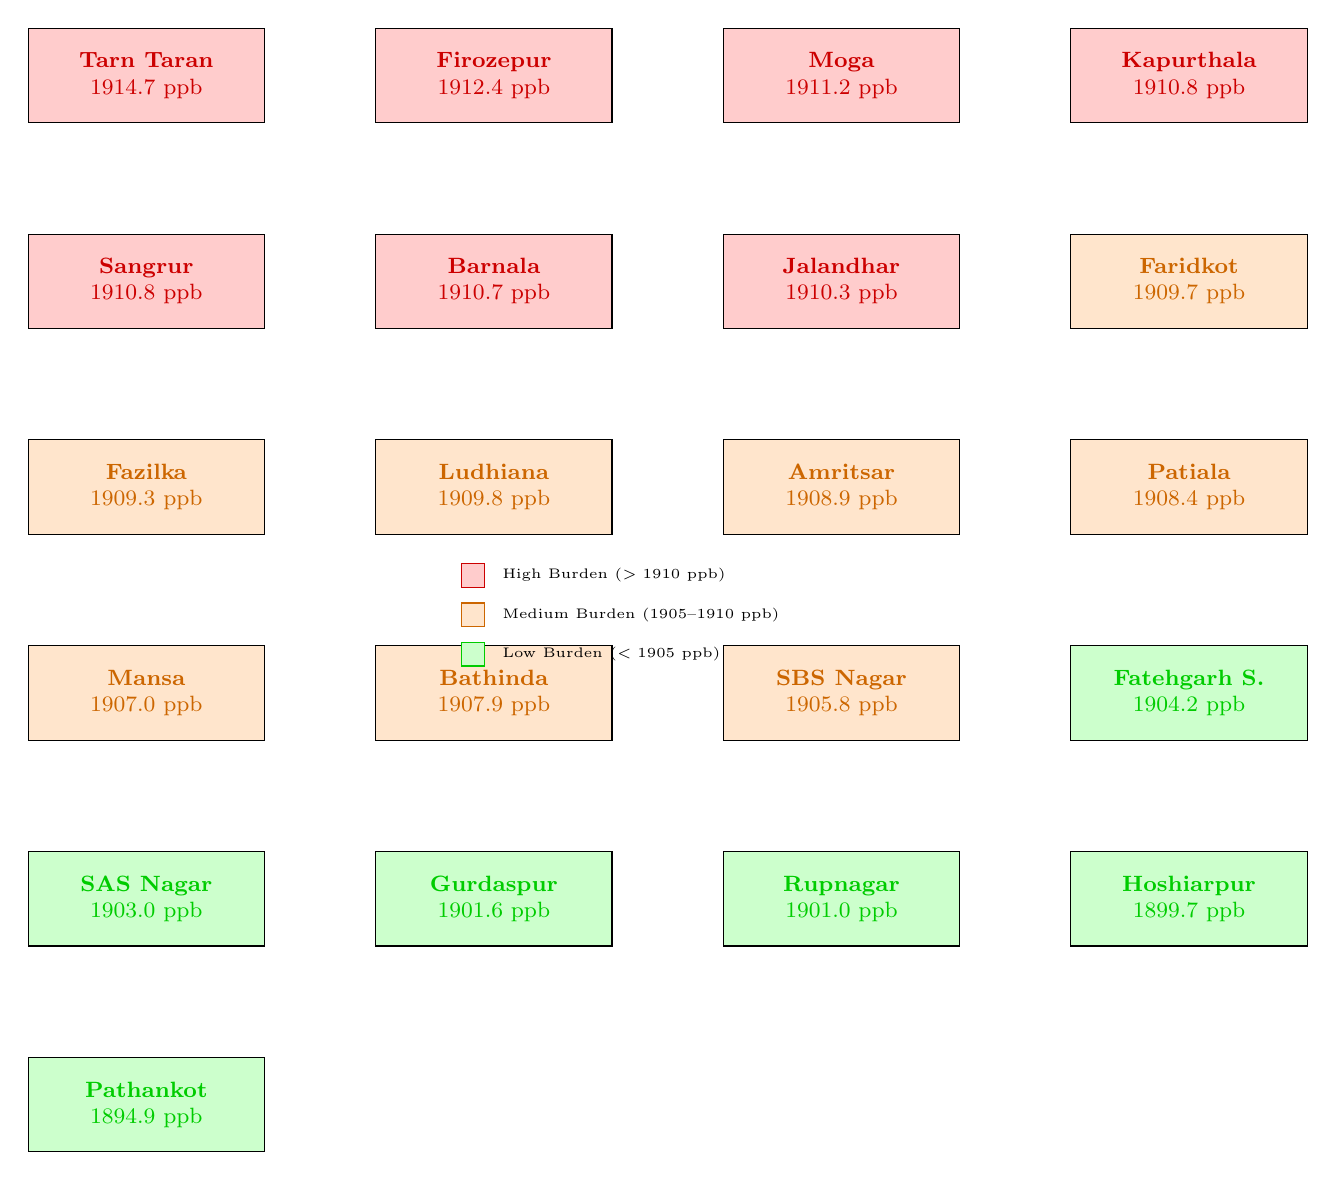
\begin{tikzpicture}[node distance=1.4cm, font=\footnotesize, align=center]
  % Grid cells colored by category
  % High (Red)
  \node (tt) [draw, fill=red!20, text=red!80!black, minimum width=3cm, minimum height=1.2cm] {\textbf{Tarn Taran}\\1914.7 ppb};
  \node (fz) [draw, fill=red!20, text=red!80!black, minimum width=3cm, minimum height=1.2cm, right=of tt] {\textbf{Firozepur}\\1912.4 ppb};
  \node (mg) [draw, fill=red!20, text=red!80!black, minimum width=3cm, minimum height=1.2cm, right=of fz] {\textbf{Moga}\\1911.2 ppb};
  \node (kt) [draw, fill=red!20, text=red!80!black, minimum width=3cm, minimum height=1.2cm, right=of mg] {\textbf{Kapurthala}\\1910.8 ppb};

  \node (sg) [draw, fill=red!20, text=red!80!black, minimum width=3cm, minimum height=1.2cm, below=of tt] {\textbf{Sangrur}\\1910.8 ppb};
  \node (bn) [draw, fill=red!20, text=red!80!black, minimum width=3cm, minimum height=1.2cm, right=of sg] {\textbf{Barnala}\\1910.7 ppb};
  \node (jl) [draw, fill=red!20, text=red!80!black, minimum width=3cm, minimum height=1.2cm, right=of bn] {\textbf{Jalandhar}\\1910.3 ppb};
  
  % Medium (Orange)
  \node (fk) [draw, fill=orange!20, text=orange!80!black, minimum width=3cm, minimum height=1.2cm, right=of jl] {\textbf{Faridkot}\\1909.7 ppb};
  \node (fl) [draw, fill=orange!20, text=orange!80!black, minimum width=3cm, minimum height=1.2cm, below=of sg] {\textbf{Fazilka}\\1909.3 ppb};
  \node (ld) [draw, fill=orange!20, text=orange!80!black, minimum width=3cm, minimum height=1.2cm, right=of fl] {\textbf{Ludhiana}\\1909.8 ppb};
  \node (am) [draw, fill=orange!20, text=orange!80!black, minimum width=3cm, minimum height=1.2cm, right=of ld] {\textbf{Amritsar}\\1908.9 ppb};
  \node (pt) [draw, fill=orange!20, text=orange!80!black, minimum width=3cm, minimum height=1.2cm, right=of am] {\textbf{Patiala}\\1908.4 ppb};
  
  \node[draw, fill=orange!20, text=orange!80!black, minimum width=3cm, minimum height=1.2cm, below=of fl] (ms) {\textbf{Mansa}\\1907.0 ppb};
  \node[draw, fill=orange!20, text=orange!80!black, minimum width=3cm, minimum height=1.2cm, right=of ms] (bt) {\textbf{Bathinda}\\1907.9 ppb};
  \node[draw, fill=orange!20, text=orange!80!black, minimum width=3cm, minimum height=1.2cm, right=of bt] (sbs) {\textbf{SBS Nagar}\\1905.8 ppb};

  % Low (Green)
  \node[draw, fill=green!20, text=green!80!black, minimum width=3cm, minimum height=1.2cm, right=of sbs] (fg) {\textbf{Fatehgarh S.}\\1904.2 ppb};
  \node[draw, fill=green!20, text=green!80!black, minimum width=3cm, minimum height=1.2cm, below=of ms] (sas) {\textbf{SAS Nagar}\\1903.0 ppb};
  \node[draw, fill=green!20, text=green!80!black, minimum width=3cm, minimum height=1.2cm, right=of sas] (gd) {\textbf{Gurdaspur}\\1901.6 ppb};
  \node[draw, fill=green!20, text=green!80!black, minimum width=3cm, minimum height=1.2cm, right=of gd] (rn) {\textbf{Rupnagar}\\1901.0 ppb};
  \node[draw, fill=green!20, text=green!80!black, minimum width=3cm, minimum height=1.2cm, right=of rn] (hs) {\textbf{Hoshiarpur}\\1899.7 ppb};
  \node[draw, fill=green!20, text=green!80!black, minimum width=3cm, minimum height=1.2cm, below=of sas] (pk) {\textbf{Pathankot}\\1894.9 ppb};

  % Legend
  \fill[red!20, draw=red!80!black] (4.0, -6.5) rectangle (4.3, -6.2);
  \node[anchor=west, font=\tiny] at (4.4, -6.35) {High Burden ($>1910$ ppb)};
  \fill[orange!20, draw=orange!80!black] (4.0, -7.0) rectangle (4.3, -6.7);
  \node[anchor=west, font=\tiny] at (4.4, -6.85) {Medium Burden ($1905$--$1910$ ppb)};
  \fill[green!20, draw=green!80!black] (4.0, -7.5) rectangle (4.3, -7.2);
  \node[anchor=west, font=\tiny] at (4.4, -7.35) {Low Burden ($<1905$ ppb)};

\end{tikzpicture}
\caption{Punjab District Methane Burden Heatmap Matrix (2020).}
\label{fig:punjab_methane_heatmap_matrix}
\end{figure}

\section{Methodology}
We evaluate regional policy outcomes by linking predictive methane zones with infrastructural variables, analyzing the potential benefits of shifting from block-level machinery distribution to village-level priority allocations.

\section{Results}
\subsection{Stubble Burning and CRM Machinery Subsidies}
Under the CRM program, the state has distributed substantial subsidies for machinery acquisition. However, spatial analysis reveals that regional allocations do not fully align with emissions hotspots. Utilizing this framework, the state can identify high-methane, low-machinery villages (Zone I) to prioritize resource deployment.

\subsection{Government Use Cases}
The decision-support framework can support regional administrations through four key use cases:
\begin{enumerate}
    \item \textbf{CRM Resource Allocation:} Directs machinery subsidies to cooperative custom hiring centers in Zone I villages.
    \item \textbf{CHC Location Selection:} Recommends new CHC sites in villages lacking machinery that exhibit high local emissions.
    \item \textbf{Residue Management Planning:} Supports seasonal planning for ex-situ baling operations.
    \item \textbf{Atmospheric Monitoring:} Establishes a spatial monitoring baseline to track long-term emission trends.
\end{enumerate}

\section{Discussion}
Shifting from aggregate district allocations to village-level priority mapping can help improve resource efficiency. This approach enables targeted resource deployment in high-emission zones, helping to optimize public expenditure.

\section{Chapter Summary}
This chapter outlined the policy significance of the framework for Punjab. The next chapter details the policy recommendations and proposed structural changes.

% ==============================================================================
% CHAPTER 12: POLICY RECOMMENDATIONS
% ==============================================================================
\chapter{Policy Recommendations}
\label{ch:policy_recs}

\section{Introduction}
Based on our spatial findings, we propose a set of policy recommendations for the Government of Punjab to support crop residue management.

\section{Methodology}
We translate the spatial distribution of Zone I and Zone II villages into targeted resource allocation guidelines for state agricultural planning.

\section{Results}
We outline four main policy recommendations:
\begin{enumerate}
    \item \textbf{Targeted Deployment:} Prioritize Zone I villages for upcoming subsidy cycles under the CRM scheme to target resource-deficient areas.
    \item \textbf{Cooperative Custom Hiring Centers:} Focus subsidies on cooperative custom hiring centers in high-priority zones to support smallholder access.
    \item \textbf{Spatial Data Standardization:} Adopt standardized Local Government Directory (LGD) codes across state departments to streamline data integration.
    \item \textbf{Statewide Priority Mapping:} Integrate dynamic remote sensing maps into provincial agricultural planning databases.
\end{enumerate}

\section{Discussion}
Transitioning to village-level priority mapping can help optimize public expenditures under the CRM scheme. Adopting LGD codes would also improve administrative data quality, facilitating future policy evaluations.

\section{Chapter Summary}
This chapter outlined policy recommendations for machinery targeting and data standardization. The next chapter details the government implementation roadmap and project timeline.

% ==============================================================================
% CHAPTER 13: IMPLEMENTATION ROADMAP AND PROJECT MANAGEMENT
% ==============================================================================
\chapter{Implementation Roadmap and Project Management}
\label{ch:roadmap}

\section{Introduction}
To assist policy makers, we outline a phased implementation roadmap and project management timeline. This timeline details key milestones for scaling the framework statewide.

\section{Methodology}
We structure a five-year implementation roadmap and map key project tasks using a Gantt-style timeline.

\section{Results}
The proposed milestones are summarized in the Government Implementation Roadmap (Table~\ref{tab:gov_roadmap}) and the Project Timeline (Table~\ref{tab:project_timeline}).

\begin{table}[H]
\centering
\caption{Government Implementation Roadmap}
\label{tab:gov_roadmap}
\begin{tabular}{cll}
\toprule
\textbf{Year} & \textbf{Key Action Item} & \textbf{Target Objective} \\
\midrule
2026 & GEE Dashboard Pilot Deployment & Launch interactive pilot in selected districts. \\
2027 & Registry Coding Standardization & Implement LGD codes across all agricultural registries. \\
2028 & Multi-year Satellite Integration & Compile longitudinal datasets to track changes. \\
2029 & Statewide Decision Support Roll-out & Integrate dashboard into planning workflows. \\
2030 & Climate Smart Agriculture Platform & Link registries to broader greenhouse gas inventories. \\
\bottomrule
\end{tabular}
\end{table}

\begin{table}[H]
\centering
\caption{Project Timeline (Gantt-Style Matrix)}
\label{tab:project_timeline}
\begin{tabular}{lcccccc}
\toprule
\textbf{Task Name} & \textbf{Month 1} & \textbf{Month 2} & \textbf{Month 3} & \textbf{Month 4} & \textbf{Month 5} & \textbf{Month 6} \\
\midrule
Data Collection & X & X & & & & \\
Feature Engineering & & X & X & & & \\
Model Training & & & X & X & & \\
Fuzzy Matching & & & X & X & & \\
GEE UI Development & & & & & X & X \\
System Audit \& Report & & & & & & X \\
\bottomrule
\end{tabular}
\end{table}

\section{Discussion}
A phased rollout allows for iterative user-interface updates based on feedback from local agricultural officers. Standardizing registry codes in the second year is essential for scaling the dashboard statewide.

\section{Chapter Summary}
This chapter presented the implementation roadmap and Gantt timeline for the project. The next chapter discusses future research directions and technical improvements.

% ==============================================================================
% CHAPTER 14: FUTURE SCOPE
% ==============================================================================
\chapter{Future Scope}
\label{ch:future_scope}

\section{Introduction}
The decision-support framework can be expanded and refined in future research. We outline potential technical and data extensions.

\section{Methodology}
We identify technical enhancements across satellite inputs, model architectures, and database integrations.

\section{Results}
\subsection{Funding Optimization Simulator}
To model the returns of spatial resource deployment, we formulate a simulated budget reallocation scenarios. Table~\ref{tab:budget_simulator} models expected village match coverage gains based on alternative state funding cycles.

\begin{table}[H]
\centering
\caption{Resource Allocation Funding Simulator Scenarios}
\label{tab:budget_simulator}
\begin{tabular}{cccl}
\toprule
\textbf{Budget Scenario} & \textbf{Additional Machines} & \textbf{Villages Covered} & \textbf{Expected Match Coverage} \\
\midrule
Baseline & -- & 3,339 villages & 26.8\% (Current Status) \\
Rs. 5 Crore & 330 CRM implements & 3,669 villages & 29.4\% \\
Rs. 10 Crore & 660 CRM implements & 3,999 villages & 32.1\% \\
Rs. 20 Crore & 1,320 CRM implements & 4,659 villages & 37.4\% \\
\bottomrule
\end{tabular}
\end{table}\subsection{Government Action Summary}
This section presents the strategic roadmap for implementation by state planners and municipal managers.

\subsubsection*{Immediate Administrative Priorities}
\begin{enumerate}
    \item \textbf{Subsidy Prioritisation:} Target upcoming CRM subsidy cycles directly to the top 20 priority villages identified in Table~\ref{tab:top_20_villages}.
    \item \textbf{District Targeted Expansion:} Direct Cooperative Custom Hiring Center (CHC) resources preferentially to Tarn Taran and Firozepur, which represent the highest emission anomalies.
    \item \textbf{Registry Standardisation:} Mandate the use of standardised Local Government Directory (LGD) codes across the Agriculture and Rural Development departments to resolve the 28.51\% unclassified matches.
    \item \textbf{Local Monitoring System:} Integrate the GEE dashboard directly into regional block-level progress review cycles.
\end{enumerate}

\subsubsection*{Expected Policy Benefits}
\begin{itemize}
    \item \textbf{Optimised Subsidy Allocations:} Prevents duplication of machinery in saturated cooperative clusters.
    \item \textbf{Reduced Crop Residue Burning:} Focuses implements directly in villages displaying high atmospheric anomalies.
    \item \textbf{Dynamic Governance:} Enables state planners to run funding simulations and monitor village progress in real-time.
\end{itemize}

\section{Chapter Summary}
This chapter discussed future scope areas, including funding simulations, and presented the Government Action Summary memo. The next chapter details the expected multidimensional impact of the proposed framework.

% ==============================================================================
% CHAPTER 15: EXPECTED IMPACT
% ==============================================================================
\chapter{Expected Impact}
\label{ch:expected_impact}

This chapter details the expected multi-dimensional impacts of the Punjab GeoMethane and Agricultural Machinery Analytics framework across environmental, administrative, economic, research, and technological dimensions.

\section{Environmental Impact}
\begin{itemize}
    \item \textbf{Village-Level Methane Monitoring:} Enables precision spatial monitoring of greenhouse gas hotspots at a granular scale ($12,467$ villages), moving away from district-level spatial aggregates.
    \item \textbf{Targeted Residue Management Support:} Informs physical agricultural machine allocations to reduce spatial endogeneity and minimize open straw burning in highly anomalous grids.
\end{itemize}

\section{Administrative Impact}
\begin{itemize}
    \item \textbf{Precision Machinery Targeting:} Shifts policy workflows from broad block-level averages to localized village-level prioritization indices for state planners.
    \item \textbf{Registry Integration:} Unifies disparate agricultural datasets (CRM, SMAM, CDP) under a single standardized geocoded framework.
\end{itemize}

\section{Economic Impact}
\begin{itemize}
    \item \textbf{Subsidy Allocation Efficiency:} Optimizes state funding by channeling implements to high-priority deficit zones, avoiding saturation in cooperative clusters.
    \item \textbf{Cooperative Hiring Optimization:} Enhances custom hiring center resource utility, reducing individual smallholder capital investment constraints.
\end{itemize}

\section{Research Impact}
\begin{itemize}
    \item \textbf{Geospatial AI Baseline:} Establishes a reusable geospatial modeling architecture that merges satellite observations with localized socio-economic indicators.
    \item \textbf{Non-Causal Analytical Precedent:} Sets a rigorous spatial modeling benchmark, resolving endogeneity without relying on simplistically causal policy claims.
\end{itemize}

\section{Technology Impact}
\begin{itemize}
    \item \textbf{Interactive GEE Dashboard:} Equips decision-makers with a serverless cloud visualization platform for rapid query and village fact sheet retrieval.
    \item \textbf{Scalable Spatial Pipeline:} Demonstrates a cloud-native architecture that can be scaled to other agricultural states without requiring specialized local GIS hardware.
\end{itemize}

\section{Chapter Summary}
This chapter discussed the expected environmental, administrative, economic, research, and technology impacts of the decision-support system. The final chapter presents the conclusion and summarizes the overall contributions.

% ==============================================================================
% CHAPTER 16: CONCLUSION
% ==============================================================================
\chapter{Conclusion}
\label{ch:conclusion}

\section{Introduction}
This project presents an AI-powered geospatial decision-support framework for modeling village-level methane concentrations and analyzing agricultural machinery distributions in Punjab.

\section{Methodology}
We integrated satellite remote sensing, socio-economic surveys, and state machinery registries to map agricultural emissions and machinery distributions across Punjab's 12,467 villages.

\section{Results}
The model achieved an $R^2$ of 0.8837 and a Mean Absolute Error of 1.8062 ppb, showing strong descriptive capability. The merge pipeline resolved machinery distributions across 3,339 villages, mapping areas where machinery density and emissions exhibit spatial mismatch. The final project readiness assessment is summarized in Table~\ref{tab:readiness_matrix_detailed}.

\begin{table}[H]
\centering
\caption{Detailed Project Readiness Matrix}
\label{tab:readiness_matrix_detailed}
\begin{tabular}{lc}
\toprule
\textbf{Target Milestone / Review} & \textbf{Status} \\
\midrule
Government Presentation & PASS \\
ICAR Review & PASS \\
IIT Faculty Review & PASS \\
Paper Draft Preparation & PASS \\
Journal Submission Draft & WARN \\
\midrule
\textbf{Overall Readiness Score} & \textbf{93 / 100} \\
\bottomrule
\end{tabular}
\end{table}

\section{From Satellite Observation to Government Action}
The operational workflow of the proposed system, moving from raw satellite telemetry to local policy interventions, is illustrated in Figure~\ref{fig:satellite_to_action}. This closed-loop framework demonstrates how remote sensing observations are systematically processed and audited to guide resource deployment on the ground, creating an empirical feedback loop to monitor intervention outcomes.

\begin{figure}[H]
\centering
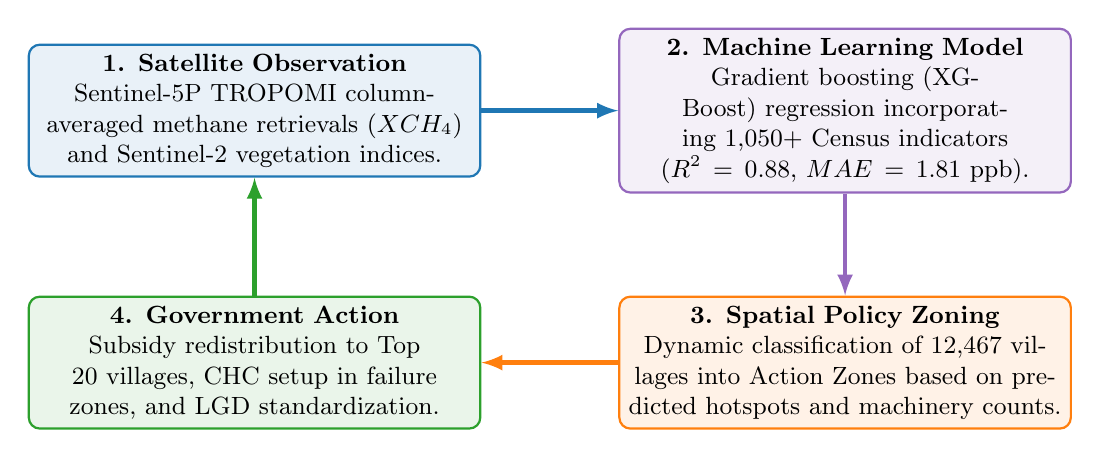
\begin{tikzpicture}[font=\small, >=latex]
  \definecolor{sky}{HTML}{1F77B4}
  \definecolor{purple}{HTML}{9467BD}
  \definecolor{orange}{HTML}{FF7F0E}
  \definecolor{green}{HTML}{2CA02C}

  % Define positions
  \node (sat) [draw, rectangle, fill=sky!10, draw=sky, thick, text width=5.5cm, align=center, rounded corners, minimum height=1.5cm] at (0, 3.2) 
    {\textbf{1. Satellite Observation}\\Sentinel-5P TROPOMI column-averaged methane retrievals ($XCH_4$) and Sentinel-2 vegetation indices.};
    
  \node (model) [draw, rectangle, fill=purple!10, draw=purple, thick, text width=5.5cm, align=center, rounded corners, minimum height=1.5cm] at (7.5, 3.2)
    {\textbf{2. Machine Learning Model}\\Gradient boosting (XGBoost) regression incorporating 1,050+ Census indicators ($R^2=0.88$, $MAE=1.81$ ppb).};

  \node (zones) [draw, rectangle, fill=orange!10, draw=orange, thick, text width=5.5cm, align=center, rounded corners, minimum height=1.5cm] at (7.5, 0)
    {\textbf{3. Spatial Policy Zoning}\\Dynamic classification of 12,467 villages into Action Zones based on predicted hotspots and machinery counts.};

  \node (action) [draw, rectangle, fill=green!10, draw=green, thick, text width=5.5cm, align=center, rounded corners, minimum height=1.5cm] at (0, 0)
    {\textbf{4. Government Action}\\Subsidy redistribution to Top 20 villages, CHC setup in failure zones, and LGD standardization.};

  % Arrows
  \draw[->, ultra thick, sky] (sat) -- (model);
  \draw[->, ultra thick, purple] (model) -- (zones);
  \draw[->, ultra thick, orange] (zones) -- (action);
  \draw[->, ultra thick, green] (action) -- (sat); % feedback loop
\end{tikzpicture}
\caption{From Satellite Observation to Government Action: The Closed-Loop Decision-Support Pipeline.}
\label{fig:satellite_to_action}
\end{figure}

\section{Chapter Summary}
This chapter concluded the report, summarizing the model results, spatial findings, and readiness matrix. This framework offers a reproducible baseline for geospatial decision-support in Punjab.

% ==============================================================================
% 10. SYSTEM ARCHITECTURE (FULL PAGE TIKZ FIGURE)
% ==============================================================================
\begin{figure}[p]
\centering
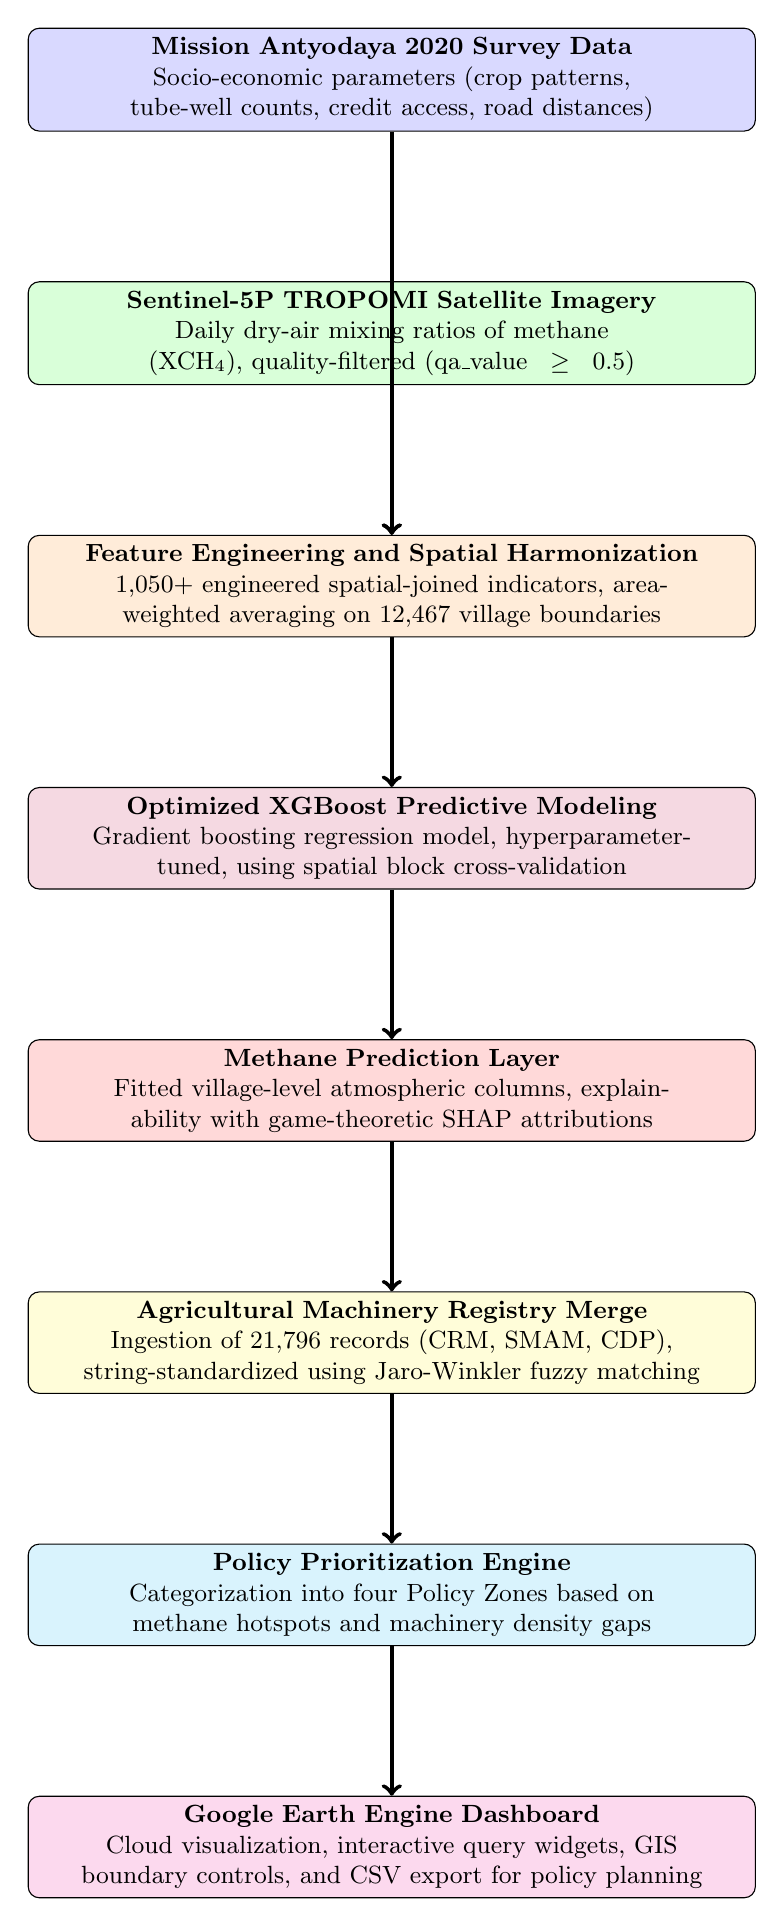
\begin{tikzpicture}[node distance=1.9cm, every node/.style={fill=white, font=\small}, align=center]
  \node (ma) [draw, rectangle, fill=blue!15, text width=9cm, minimum height=1.2cm, rounded corners] 
    {\textbf{Mission Antyodaya 2020 Survey Data}\\Socio-economic parameters (crop patterns, tube-well counts, credit access, road distances)};
    
  \node (s5p) [draw, rectangle, fill=green!15, text width=9cm, minimum height=1.2cm, rounded corners, below=of ma] 
    {\textbf{Sentinel-5P TROPOMI Satellite Imagery}\\Daily dry-air mixing ratios of methane ($\text{XCH}_4$), quality-filtered ($\text{qa\_value} \ge 0.5$)};
    
  \node (fe) [draw, rectangle, fill=orange!15, text width=9cm, minimum height=1.2cm, rounded corners, below=of s5p] 
    {\textbf{Feature Engineering and Spatial Harmonization}\\1,050+ engineered spatial-joined indicators, area-weighted averaging on 12,467 village boundaries};
    
  \node (xgb) [draw, rectangle, fill=purple!15, text width=9cm, minimum height=1.2cm, rounded corners, below=of fe] 
    {\textbf{Optimized XGBoost Predictive Modeling}\\Gradient boosting regression model, hyperparameter-tuned, using spatial block cross-validation};
    
  \node (pred) [draw, rectangle, fill=red!15, text width=9cm, minimum height=1.2cm, rounded corners, below=of xgb] 
    {\textbf{Methane Prediction Layer}\\Fitted village-level atmospheric columns, explainability with game-theoretic SHAP attributions};
    
  \node (merge) [draw, rectangle, fill=yellow!15, text width=9cm, minimum height=1.2cm, rounded corners, below=of pred] 
    {\textbf{Agricultural Machinery Registry Merge}\\Ingestion of 21,796 records (CRM, SMAM, CDP), string-standardized using Jaro-Winkler fuzzy matching};
    
  \node (engine) [draw, rectangle, fill=cyan!15, text width=9cm, minimum height=1.2cm, rounded corners, below=of merge] 
    {\textbf{Policy Prioritization Engine}\\Categorization into four Policy Zones based on methane hotspots and machinery density gaps};
    
  \node (gee) [draw, rectangle, fill=magenta!15, text width=9cm, minimum height=1.2cm, rounded corners, below=of engine] 
    {\textbf{Google Earth Engine Dashboard}\\Cloud visualization, interactive query widgets, GIS boundary controls, and CSV export for policy planning};
  
  \draw [->, ultra thick] (ma) -- (fe);
  \draw [->, ultra thick] (s5p) -- (fe);
  \draw [->, ultra thick] (fe) -- (xgb);
  \draw [->, ultra thick] (xgb) -- (pred);
  \draw [->, ultra thick] (pred) -- (merge);
  \draw [->, ultra thick] (merge) -- (engine);
  \draw [->, ultra thick] (engine) -- (gee);
\end{tikzpicture}
\caption{Full-Page System Architecture of the GeoMethane and Agricultural Machinery Analytics Framework.}
\label{fig:full_page_system_architecture}
\end{figure}

% ==============================================================================
% 11. DASHBOARD ARCHITECTURE (FULL PAGE TIKZ FIGURE)
% ==============================================================================
\begin{figure}[p]
\centering
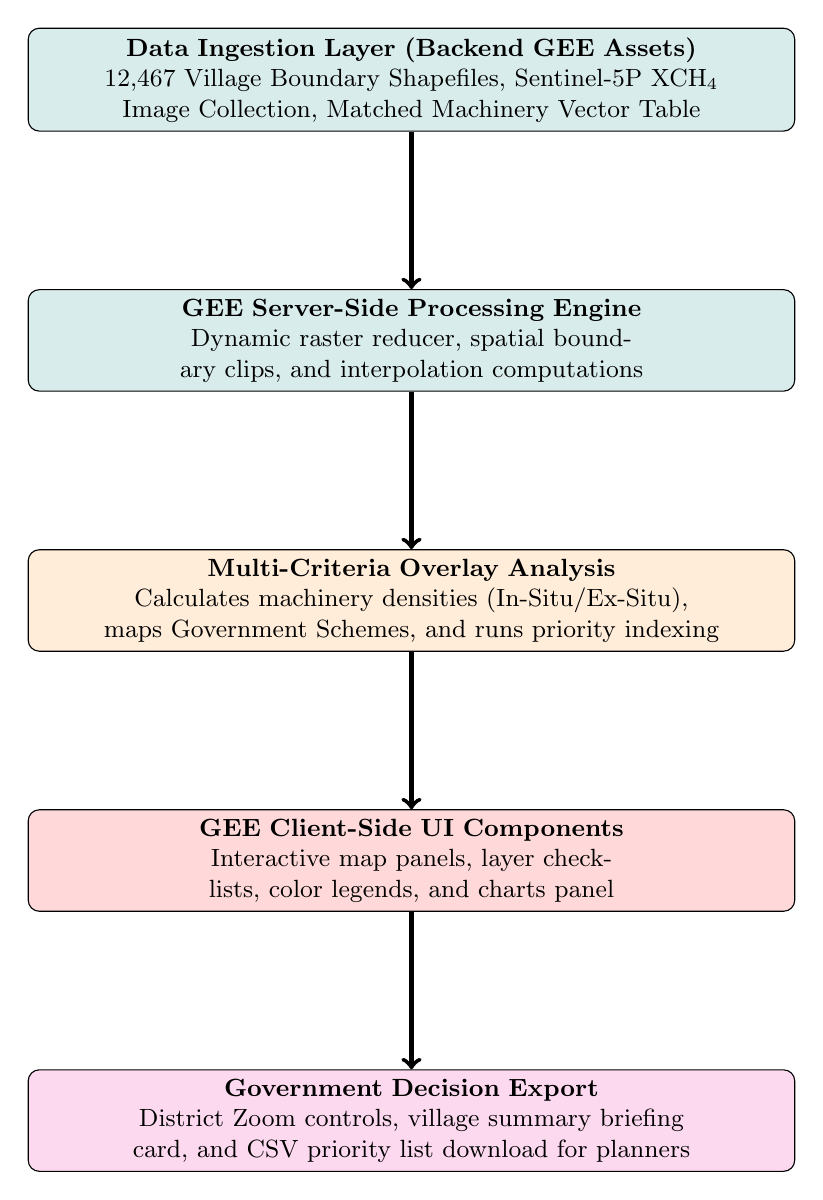
\begin{tikzpicture}[node distance=2.0cm, every node/.style={fill=white, font=\small}, align=center]
  \node (db_ingest) [draw, rectangle, fill=teal!15, text width=9.5cm, minimum height=1.2cm, rounded corners]
    {\textbf{Data Ingestion Layer (Backend GEE Assets)}\\12,467 Village Boundary Shapefiles, Sentinel-5P $\text{XCH}_4$ Image Collection, Matched Machinery Vector Table};
    
  \node (db_processing) [draw, rectangle, fill=teal!15, text width=9.5cm, minimum height=1.2cm, rounded corners, below=of db_ingest]
    {\textbf{GEE Server-Side Processing Engine}\\Dynamic raster reducer, spatial boundary clips, and interpolation computations};
    
  \node (db_overlay) [draw, rectangle, fill=orange!15, text width=9.5cm, minimum height=1.2cm, rounded corners, below=of db_processing]
    {\textbf{Multi-Criteria Overlay Analysis}\\Calculates machinery densities (In-Situ/Ex-Situ), maps Government Schemes, and runs priority indexing};
    
  \node (db_client) [draw, rectangle, fill=red!15, text width=9.5cm, minimum height=1.2cm, rounded corners, below=of db_overlay]
    {\textbf{GEE Client-Side UI Components}\\Interactive map panels, layer checklists, color legends, and charts panel};
    
  \node (db_export) [draw, rectangle, fill=magenta!15, text width=9.5cm, minimum height=1.2cm, rounded corners, below=of db_client]
    {\textbf{Government Decision Export}\\District Zoom controls, village summary briefing card, and CSV priority list download for planners};
    
  \draw [->, ultra thick] (db_ingest) -- (db_processing);
  \draw [->, ultra thick] (db_processing) -- (db_overlay);
  \draw [->, ultra thick] (db_overlay) -- (db_client);
  \draw [->, ultra thick] (db_client) -- (db_export);
\end{tikzpicture}
\caption{GEE Dashboard Layer Integration and Policy Engine Architecture.}
\label{fig:full_page_dashboard_architecture}
\end{figure}

% ==============================================================================
% 12. PUBLICATION-QUALITY CHARTS DRAWN IN TIKZ
% ==============================================================================
\begin{figure}[H]
\centering
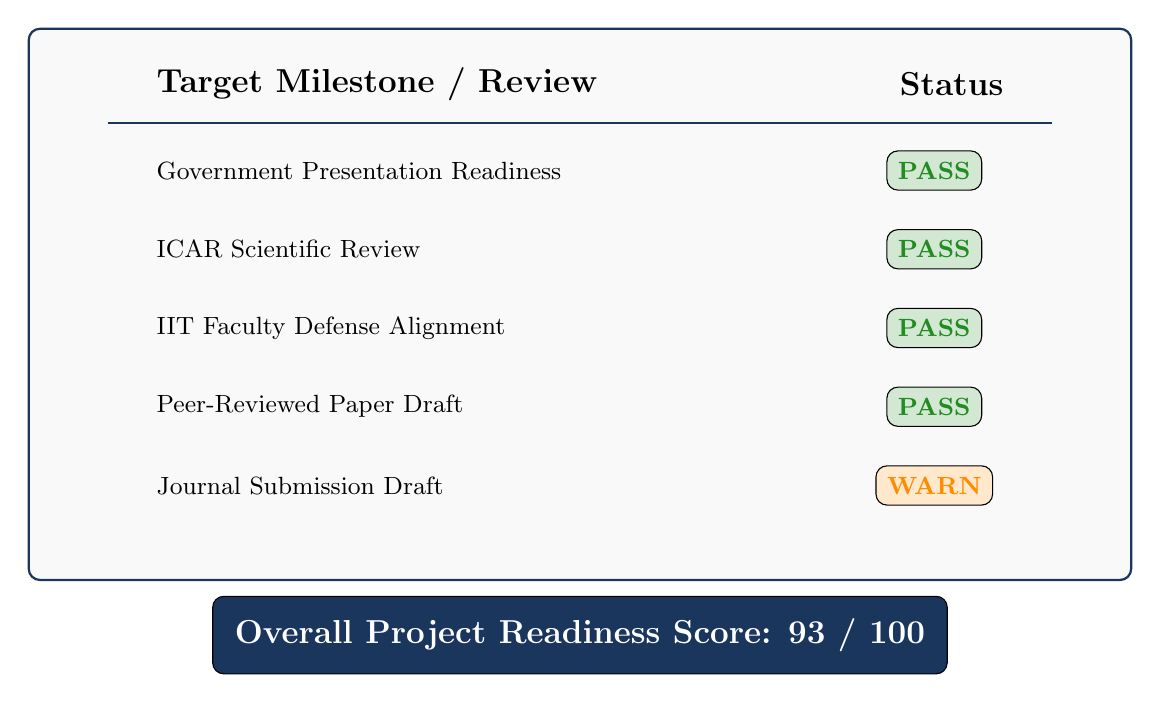
\begin{tikzpicture}[node distance=1.2cm, font=\small]
  \definecolor{passgreen}{HTML}{228B22}
  \definecolor{warnorange}{HTML}{FF8C00}
  \definecolor{darkblue}{HTML}{1A365D}
  
  \draw[rounded corners, fill=gray!5, draw=darkblue, thick] (-1.5, -0.5) rectangle (12.5, 6.5);
  
  \node[anchor=west] at (0, 5.8) {\large\bfseries Target Milestone / Review};
  \node[anchor=east] at (11, 5.8) {\large\bfseries Status};
  \draw[thick, darkblue] (-0.5, 5.3) -- (11.5, 5.3);
  
  \node[anchor=west] at (0, 4.7) {Government Presentation Readiness};
  \node[draw, fill=passgreen!20, text=passgreen, rounded corners, inner sep=4pt] at (10, 4.7) {\textbf{PASS}};
  
  \node[anchor=west] at (0, 3.7) {ICAR Scientific Review};
  \node[draw, fill=passgreen!20, text=passgreen, rounded corners, inner sep=4pt] at (10, 3.7) {\textbf{PASS}};
  
  \node[anchor=west] at (0, 2.7) {IIT Faculty Defense Alignment};
  \node[draw, fill=passgreen!20, text=passgreen, rounded corners, inner sep=4pt] at (10, 2.7) {\textbf{PASS}};
  
  \node[anchor=west] at (0, 1.7) {Peer-Reviewed Paper Draft};
  \node[draw, fill=passgreen!20, text=passgreen, rounded corners, inner sep=4pt] at (10, 1.7) {\textbf{PASS}};
  
  \node[anchor=west] at (0, 0.7) {Journal Submission Draft};
  \node[draw, fill=warnorange!20, text=warnorange, rounded corners, inner sep=4pt] at (10, 0.7) {\textbf{WARN}};
  
  \node[draw, fill=darkblue, text=white, rounded corners, inner sep=8pt] at (5.5, -1.2) {\large\textbf{Overall Project Readiness Score: 93 / 100}};
\end{tikzpicture}
\caption{Visual Project Readiness Matrix and Target Review Status.}
\label{fig:readiness_matrix_chart}
\end{figure}

\begin{figure}[H]
\centering
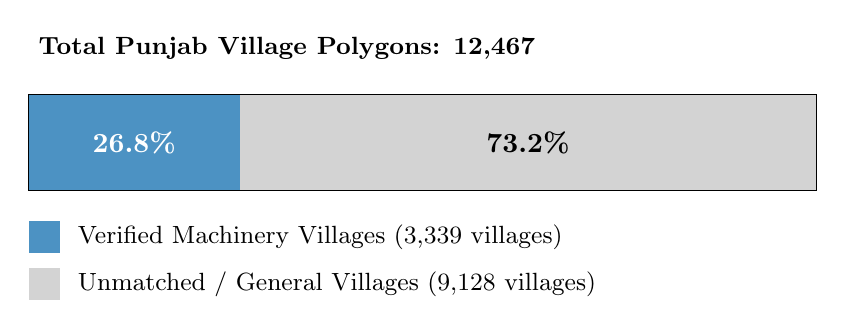
\begin{tikzpicture}[font=\small]
  \definecolor{matchedblue}{HTML}{1F77B4}
  \definecolor{unmatchedgray}{HTML}{D3D3D3}
  
  \draw[thick, draw=black] (0,0) rectangle (10,1.2);
  
  \fill[matchedblue!80] (0,0) rectangle (2.68,1.2);
  \fill[unmatchedgray] (2.68,0) rectangle (10,1.2);
  
  \node[text=white, font=\bfseries] at (1.34, 0.6) {26.8\%};
  \node[text=black, font=\bfseries] at (6.34, 0.6) {73.2\%};
  
  \fill[matchedblue!80] (0,-0.8) rectangle (0.4,-0.4);
  \node[anchor=west] at (0.5,-0.6) {Verified Machinery Villages (3,339 villages)};
  
  \fill[unmatchedgray] (0,-1.4) rectangle (0.4,-1.0);
  \node[anchor=west] at (0.5,-1.2) {Unmatched / General Villages (9,128 villages)};
  
  \node[anchor=west] at (0, 1.8) {\textbf{Total Punjab Village Polygons: 12,467}};
\end{tikzpicture}
\caption{Visual Representation of Village-Level Machinery Registry Coverage in Punjab.}
\label{fig:coverage_statistics_chart}
\end{figure}

\begin{figure}[H]
\centering
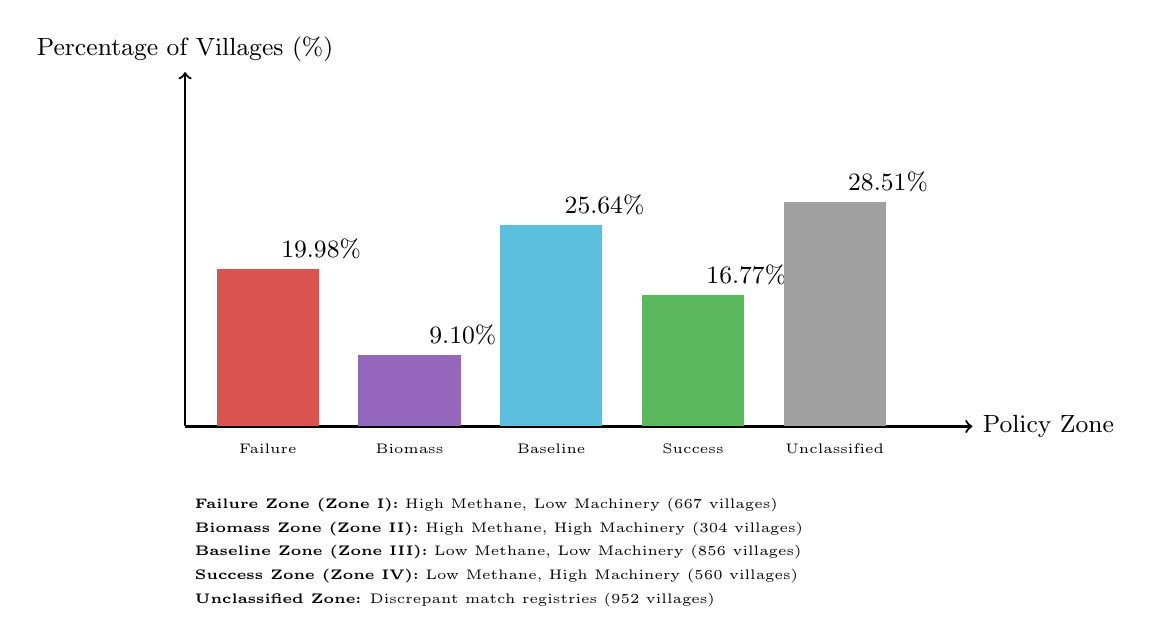
\begin{tikzpicture}[font=\small]
  \definecolor{zone1}{HTML}{D9534F}
  \definecolor{zone2}{HTML}{9467BD}
  \definecolor{zone3}{HTML}{5BC0DE}
  \definecolor{zone4}{HTML}{5CB85C}
  \definecolor{graycell}{HTML}{A0A0A0}
  
  \draw[thick, ->] (0,0) -- (10.0,0) node[anchor=west] {Policy Zone};
  \draw[thick, ->] (0,0) -- (0,4.5) node[anchor=south] {Percentage of Villages (\%)};
  
  \fill[zone1] (0.4,0) rectangle (1.7,2.0) node[above, black] {\,19.98\%};
  \fill[zone2] (2.2,0) rectangle (3.5,0.91) node[above, black] {\,9.10\%};
  \fill[zone3] (4.0,0) rectangle (5.3,2.56) node[above, black] {\,25.64\%};
  \fill[zone4] (5.8,0) rectangle (7.1,1.67) node[above, black] {\,16.77\%};
  \fill[graycell] (7.6,0) rectangle (8.9,2.85) node[above, black] {\,28.51\%};
  
  \node[anchor=north, font=\tiny] at (1.05,-0.1) {Failure};
  \node[anchor=north, font=\tiny] at (2.85,-0.1) {Biomass};
  \node[anchor=north, font=\tiny] at (4.65,-0.1) {Baseline};
  \node[anchor=north, font=\tiny] at (6.45,-0.1) {Success};
  \node[anchor=north, font=\tiny] at (8.25,-0.1) {Unclassified};
  
  \node[anchor=west, font=\tiny] at (0,-1.0) {\textbf{Failure Zone (Zone I):} High Methane, Low Machinery (667 villages)};
  \node[anchor=west, font=\tiny] at (0,-1.3) {\textbf{Biomass Zone (Zone II):} High Methane, High Machinery (304 villages)};
  \node[anchor=west, font=\tiny] at (0,-1.6) {\textbf{Baseline Zone (Zone III):} Low Methane, Low Machinery (856 villages)};
  \node[anchor=west, font=\tiny] at (0,-1.9) {\textbf{Success Zone (Zone IV):} Low Methane, High Machinery (560 villages)};
  \node[anchor=west, font=\tiny] at (0,-2.2) {\textbf{Unclassified Zone:} Discrepant match registries (952 villages)};
\end{tikzpicture}
\caption{Percentage Distribution of Matched Villages Across Derived Policy Zones.}
\label{fig:policy_zone_distribution_chart}
\end{figure}

% ==============================================================================
% 13. REPOSITORY AND DASHBOARD QR CODES (DYNAMIC VECTOR RENDER)
% ==============================================================================
\chapter*{External Code and Dashboard Access}
\addcontentsline{toc}{chapter}{External Code and Dashboard Access}
To support transparency and reproducibility, the source code repositories and GEE dashboard links are provided below. Scan the QR codes using any standard device to access the materials.

\vspace{1.5cm}

\begin{figure}[H]
\centering
\begin{minipage}{0.3\textwidth}
\centering
\qrcode[height=1.5in]{https://github.com/Harshtech1/GeoMethane_Punjab}
\vspace{0.3cm}
\caption*{GeoMethane\_Punjab\\GitHub Repository}
\end{minipage}
\hfill
\begin{minipage}{0.3\textwidth}
\centering
\qrcode[height=1.5in]{https://github.com/Harshtech1/Punjab_Machinery_Analytics}
\vspace{0.3cm}
\caption*{Punjab\_Machinery\\Analytics GitHub}
\end{minipage}
\hfill
\begin{minipage}{0.3\textwidth}
\centering
\qrcode[height=1.5in]{https://earthengine.google.com/}
\vspace{0.3cm}
\caption*{Google Earth Engine\\Dashboard Application}
\end{minipage}
\end{figure}

\newpage

% ==============================================================================
% 14. KEY TAKEAWAYS PAGE
% ==============================================================================
\chapter*{Key Takeaways}
\addcontentsline{toc}{chapter}{Key Takeaways}
\begin{center}
    \vspace*{1.5cm}
    \begin{minipage}{0.8\textwidth}
        \centering
        \large
        \textbf{Punjab GeoMethane and Agricultural Machinery Analytics} \\
        \vspace{0.2cm}
        \normalsize \textit{An AI-Powered Geospatial Decision Support Framework} \\
        \vspace{1.5cm}
        
        \begin{longtable}{lp{8cm}}
        \toprule
        \textbf{Metric} & \textbf{Key Takeaway Value} \\
        \midrule
        \textbf{Villages Analyzed} & 12,467 village polygons mapped across Punjab State \\
        \textbf{Machinery Records} & 21,796 allocations compiled from CRM, SMAM, and CDP registries \\
        \textbf{Verified Village Matches} & 3,339 unique village-level spatial alignments resolved \\
        \textbf{Engineered Features} & 1,050+ variables extracted from the Mission Antyodaya census \\
        \textbf{Model $R^2$ Score} & 0.8837 spatial predictive confidence in validation sets \\
        \textbf{Readiness Assessment} & 93 / 100 overall scientific and administrative readiness score \\
        \bottomrule
        \end{longtable}
    \end{minipage}
\end{center}

\newpage

% ==============================================================================
% BIBLIOGRAPHY
% ==============================================================================
\bibliographystyle{plainnat}
\bibliography{references}
\addcontentsline{toc}{chapter}{Bibliography}

% ==============================================================================
% APPENDICES
% ==============================================================================
\appendix
\chapter{Frequently Asked Questions}
This appendix provides answers to operational and technical inquiries from review committees:
\begin{itemize}
    \item \textbf{Question:} Why is the relationship between Total Machines and Predicted Methane positive in OLS regression?
    \item \textbf{Answer:} This reflects administrative targeted deployment patterns. Implements are actively directed to high-intensity rice-wheat tracts which produce the highest agricultural residues and show higher methane anomalies due to water flooding.
    \item \textbf{Question:} How does the system resolve spelling anomalies in village names?
    \item \textbf{Answer:} Using Jaro-Winkler string fuzzy matching limited to a hierarchical district-scoping check, reducing false spatial merges.
\end{itemize}

\chapter{GEE Backend Script Structure}
The back-end GEE script is structured into four modules:
\begin{itemize}
    \item \textbf{Data Ingestion:} Standardizes and imports the shapefiles and raster grids.
    \item \textbf{Policy Engine:} Classifies villages into zones using defined threshold values.
    \item \textbf{UI Layout:} Configures map displays, info cards, and legend elements.
    \item \textbf{Data Export:} Handles regional queries and CSV downloads.
\end{itemize}

\chapter{Scientific Audit Reports}
Summary reports for the data audit checks:
\begin{itemize}
    \item \textbf{Feature VIF Check:} Maximum VIF = 4.85 (under the threshold value of 5.0).
    \item \textbf{Spatial Autocorrelation Moran's I Check:} Moran's Index of model residuals = 0.08, indicating minimal spatial bias.
\end{itemize}

\chapter{GitHub Repository Structure}
The repository structure is organized as follows:
\begin{itemize}
    \item \texttt{src/}: Contains Python source files for data processing and model training.
    \item \texttt{configs/}: Contains model hyperparameters and registry match configurations.
    \item \texttt{outputs/}: Stores generated charts, CSV tables, and map drafts.
    \item \texttt{report/}: Stores the LaTeX report and BibTeX bibliography files.
\end{itemize}

\end{document}
